%
% Cells Chapter
% Jason Brownlee
%

\chapter{Cellular Clonal Selection}
\label{chap:cells}

%
% Overview
% Provides an overview of the chapter and its structure, and a description of what is intended to be achieved by providing this documentation. A description of why and how this chapter follows on from the previous chapter
%
\section{Chapter Overview}
\label{sec:cellsoverview}
This chapter consolidates the findings of the previous chapter and proposes the first of three constrained perspectives of the clonal selection strategy. Specifically, this chapter is concerned with clonal selection as constrained by the antigenic, cellular, and molecular interactions of cells within a repertoire called the \emph{Cellular Clonal Selection Paradigm}. Importantly the perspective of clonal selection as an adaptive strategy considered in this chapter both encapsulates the state of the art in clonal selection algorithms, and provides a bedrock of understanding for the integrated hierarchy of perspectives considered in the remainder of this dissertation. 
% breakdown
Section~\ref{sec:cells:paradigm} considers the cellular perspective from an abstract perspective, dividing the concerns of the paradigm into that of \emph{system} and \emph{environment}, clearly delineating the responsibility of the adaptive strategy and the problem domain that provides the context for adaptation. The paradigm is realised in Section~\ref{sec:cells:realised} with regard to specific algorithm and problem definitions and empirical measures for assessing the composition and capability of a given repertoire governed by clonal selection. The behavioural expectations of an archetype of the strategy are assessed and confirmed in a series of three empirical studies in Section~\ref{sec:cells:ccsa}. These findings provide a foundation from which three extensions of the strategy are proposed and investigated using empirical study to confirm behaviour expectations, including (1) a spatial context for the repertoire in Section~\ref{sec:cells:spatial}, (2) mediation of response provided by the interaction different cell casts in Section~\ref{sec:cells:mediated}, and (3) the promotion of higher-order cross-exposure structures in the repertoire via network inspired interactions in Section~\ref{sec:cells:network}.


%
% Abstract Cellular Paradigm
%
\section{Abstract Cellular Paradigm}
\label{sec:cells:paradigm}
The Cellular Clonal Selection Paradigm is a rephrasing and restricting of the existing field of algorithms that realise the computational attributes of the clonal selection theory of acquired immunity. This section considers the abstract concerns of the paradigm focusing on (1) a quintessential cellular clonal selection adaptive strategy, (2) a system-environment phrasing of the strategies interaction with a given domain called the antigenic exposure paradigm, and (3) a generic problem domain for conceptualising and investigating cellular clonal selection algorithms and their elaborations.

%
% Quintessential Clonal Selection
%
\subsection{Quintessential Clonal Selection}
\label{subsec:cells:paradigm:clonalselection}
This section considers an archetype of clonal selection adaptive strategy as the consolidation of the related immunological theory, computational principles and approaches, and adaptive systems theory from Chapter \ref{chap:cs}. Clonal selection is constrained to the concerns of a repertoire of cells and antigen called the \emph{Cellular Clonal Selection Paradigm} that focuses on the separation and interaction of system-environment, and clonal selection as an adaptive strategy. 

%
% Constrained Scope
%
\subsubsection{Constrained Scope}
% cellular level
The clonal selection theory is defined at the cell, antibody, and antigen level of immunobiology and immunochemistry to describe what in complex system theory are described as \emph{emergent effects} of host immunity. Therefore one may constrain the investigation of the information processing concerns of clonal selection at this level and consider the emergent immunity effects within the context of a repertoire of cells with regard to antigen. In this work, the study of clonal selection under this constraint is referred to as \emph{Cellular Clonal Selection}, distinct from the consideration of clonal selection under multiple of such repertoires in \emph{Tissue Clonal Selection} (Chapter \ref{chap:tissues}), and the consideration of clonal selection across multiple whole immune systems in \emph{Host Clonal Selection} (Chapter \ref{chap:hosts}).
% all that is, is cellular
Cellular Clonal Selection is primarily concerned with the management of a repertoire of discrete cells and its interaction with antigen. The scope of control for this management is the repertoire in its entirety. This suggests that the repertoire of cells in cellular clonal selection is centrally governed with access to complete information regarding the information content of the repertoire. Therefore the scope of cellular clonal selection algorithms considered in the reviewed taxonomy (Section~\ref{sec:cs:algorithms}) may be considered Cellular Clonal Selection Algorithms. As discussed in that section, this level of clonal selection algorithms are strongly related in mechanism and effect to the Genetic Algorithm (GA) and the Mutation Hill Climbing Algorithm (MHCA), as well as the related fields of Lazy and Competitive Learning. 

%
% System and Environment
%
\subsubsection{System and Environment}
A critical perspective on computational models of clonal selection highlighted by the adaptive systems theory in the previous chapter was the need for a clear delineation between system and the environment that the system interacts with. The system is defined as being comprised of a cellular repertoire managed by clonal selection and related information processing mechanisms. The environment is defined as the scope of endogenous antigen and exogenous pathogen to which the system may be exposed. This delineation is easily related back to the existing state of clonal selection algorithm research as a the separation between clonal selection algorithm and problem domain to which the algorithm is applied. The information content of the system and the environment may therefore be considered in the context of the shape-space and affinity landscape geometric paradigms from theoretical immunology as sets of discrete cells and antigen patterns that may be assessed (specificity and antigenicity) against each other as a cost surface. The antigenic environment defines the scope of the information a system may acquire and apply (immunity), the full importance to clonal selection of which is considered in the Antigenic Exposure Paradigm in Section~\ref{subsec:cells:paradigm:antigenicexposures}.

%
% Clonal Selection as Strategy
%
\subsubsection{Clonal Selection as Strategy}
The management of a cellular repertoire in the context of an antigenic environment is the responsibility of the clonal selection adaptive strategy. The focus of such a strategy is the acquisition and application of information (immunity) from an unknown information (antigenic) environment. The selectionist, adaptationist, and satisficing lens of the clonal selection strategy considered in the previous chapter highlighted the following computational principles of the theory:

\begin{enumerate}
	\item Information is acquired through cumulative generate-and-test of pre-committed discrete structures. 
	\item Resource allocation is competitive, based on (in some way) the differential `goodness of fit'.
	\item The continued acquisition and application of information is based on the premise that future antigenic exposures are much like past exposures.
	\item Adaptation continues for as long as relative improvements can be made under all of the constraints of the strategy. 
	\item The emergent effects of the bottom-up exposure-wise interactions may be assessed in the holistic \emph{composition} and \emph{capabilities} of the information acquired in the cellular repertoire.	
\end{enumerate}

The implementation of such a strategy was shown in Section~\ref{sec:cs:algorithms} to be commonly realised as management of a repertoire of binary strings under assessment of an oracle cost function resulting in duplication and mutation of low cost (high affinity) strings. The generality of such a realisation may be constrained by the principles or axioms governing cellular interactions with antigen from Section~\ref{sec:cs:theory}, as follows: 

\begin{itemize}	
	\item \emph{Assessment}: Affinity is an ordinal scoring of the `goodness of fit' of a structure provided by an oracle.
	\item \emph{Selection Competition}: Competition is promoted between cells specialised for the same antigen, and avoided between cells specialised for different antigen.
	\item \emph{Selection}: A small and specific founding set of cells are selected to found a clonal response (oligoclonal).
	\item \emph{Cloning}: The number of clones created from an exposure is larger than the founding set of cells selected for the clonal response.
	\item \emph{Mutation}: The point-wise rate of mutation is higher than that of normal mitosis although is fixed.
	\item \emph{Integration Competition}: The cellular repertoire is large although finite, promoting competition between cells for limited positions.
	\item \emph{Integration}: Although many clones are created in a clonal response, few are retained in the repertoire.
\end{itemize}

The listed computational principles may be considered an extension and elaboration on the affinity maturation principle of de~Castro and Timmis, and the clonal selection principle of Cutello and Nicosia in Section~\ref{subsec:cs:algorithms:principle}. These principles are the interpreted heuristics from reviewed immunological theory use in this work and are not intended to provide laws for the realisation of cellular clonal selection algorithms. Specifically, differential resource allocation can be realised via a variety of specialised mechanisms including: assessment, selection, cloning, mutation, and integration\footnote{As evidence, one may consider the variety of such mechanisms used for differential resource allocation in the related field of evolutionary computation.}. These principles are used to assess and configure cellular clonal selection algorithms in this work, and are augmented with knowledge from the study of the related GA's and MHCA's. Specifically from Section~\ref{subsec:cs:related:hillclimbing}: (1) the acceptance of structures with an improved or equal assessment scoring to permit the acceptance of varied structures with neutral effect on assessment to cross flat spots in the affinity landscape, and (2) the use of a $\frac{1}{L}$ fixed mutation rate as an approximation of the optimal mutation rate of bit strings on linear binary cost functions.


%
% Antigenic Exposure Paradigm
%
\subsection{Antigenic Exposure Paradigm}
\label{subsec:cells:paradigm:antigenicexposures}
% general
This section proposes an artificial conceptual model of a generalised natural antigenic environment. This model is comprised of a set of external triggers that stimulate an internal activation and response by an acquired immune system. This conceptualisation is called an \emph{antigenic exposure}, and provides a perspective on the adaptation-based learning and memory qualities of the acquired immune system, and a standardised framework for mapping problem domains onto the cellular clonal selection paradigm. 

% exposure models
The immune system is embedded or situated in an \emph{antigenic environment}, to which it (in general) passively responds. Therefore, a system has qualities of an intelligent agent (it is situated, intelligent, and acts autonomously), although does not act upon the environment, unlike a reinforcement learning system. A consideration of antigen other than superficial mapping of a given problem domain is largely ignored in the investigation of Artificial Immune Systems in general, as the investigatory concerns lie predominantly with the information processing qualities of the system. Antigen may be exogenous or endogenous in origin and may be benign or actively adversarial. The environment encompasses the scope of the information that may be acquired by the system, dictating what to learn and when to learn it. Three antigenic exposure regimes and resultant models are proposed, as follows: (1) single exposure, (2) multiple exposures, and (3) multiple antigen with multiple exposures, that highlight the spatial-temporal consistency concerns of clonal selection at the cellular level. 

%
% Single Exposures
%
\subsubsection{Single Exposure Model}
% general properties
An antigenic exposure is an event that involves the arrival of antigens (information of external origin) to an immune system. The arriving antigen are identified (typically forced as a requirement of the domain) by the system stimulating a proportionate immune response. If correctly identified, the \emph{external stimulation} results in an \emph{internal activation} of some lymphocytes in the immune systems repertoire. The response involves raising a clone of lymphocytes to address the stimulation with regard to the magnitude and specificity of the response. The system is concerned with raising a good response quickly. The principle of an antigen is that it may cause harm to the host in the form of tissue damage promoting the immediacy of the response. The system must raise a clone that can address the magnitude of the exposure, therefore the effectiveness of the response should be proportional to the virulence of the antigen, and the response size (clonal expansion) should be proportional to the number of arriving antigen (amplitude or dose).

\begin{figure}[ht]
	\centering
	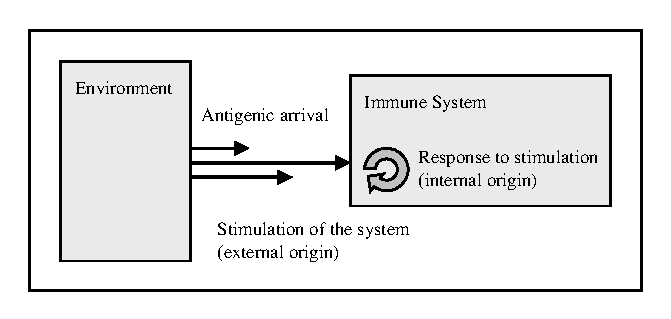
\includegraphics[scale=0.85]{Cells/antigenic-systemenv}
	\caption{Depiction of external stimulation resulting in internal activation.}
	\label{pic:cells:internalexternal}
\end{figure}

% virulence and amplitude
This \emph{exposure virulence} is a property of the antigen thus is not likely to change for a given immune system unless the antigen itself changes. The virulence may define the penalty for not identifying a antigen, as well as the amount of resultant specificity desired or required in a clonal selection and expansion response. This concern (virulence-specificity) is difficult to conceptualise as it defines the relative amount of refinement-based learning required of the system for a given antigen. The concern of the size of an antigen dose may be conceptualised as the amount or \emph{exposure amplitude} of information an antigen represents. The number of simultaneous antigen that arrive to the system in a given exposure defines the amount of work the system may have to support. The number of antigenic molecules that arrive in an exposure may be more than the number of lymphocytes in the repertoire. The result is that selection events may be more intense, resulting in the delay of some interaction until after the initial cells have proliferated or additional resources have been recruited. This \emph{exposure amplitude mismatch} scenario has two speculated implications: (1) Antigen may not be neutralised as quickly if it arrives in unexpectedly large quantities, that would result in the antigen arrival being considered a resources which must be degraded (neutralised over time), and (2) The increased selective pressure from the size mismatch may result in the rapid synthesis of a response large enough to address the exposure. This suggests dynamic and variable response size capabilities inherent in the clonal selection and expansion response. 

% why they are important
One may consider the effects of varied exposure virulence and amplitude on an immune system. Both properties affect the amount of work required in an immune response, although in different dimensions. Virulence may determine the desired specificity of a response such that high damage-causing pathogens are neutralised effectively and low damage-causing pathogens are neutralised with less specificity. The amplitude of the exposure defines the number of cells and the size of the clonal response. Therefore, the immune system must trade-off response strategies to the various anticipated virulence and amplitude combinations.
% implications for the system
For a single exposure event, an immune system is only concerned with quelling the antigen with a response. The scope of the concerns of an immune system for a single exposure is the specificity of the lymphocytes to the antigen and synthesising the cells in sufficient numbers. Initial antigen-identification (to trigger a response) may be assumed. Further, all resources of the repertoire may be allocated to the response for the exposure, as there are no future exposures. Iterations within a system under these conditions are concerned with adaptation in the context of a fixed and known single exposure event.

%
% Multiple Exposures
%
\subsubsection{Multiple Exposure Model}
A single exposure-response event may be abstracted to multiple antigen exposure-response events. A principle property of a multiple exposure regime is the temporal dimension it adds to such events. \emph{Exposure frequency} facilitates conceptualising multiple exposures as a series of atomic and quasi-independent single events, where the repetitiveness of the arrival of a given antigen is defined as its frequency. The exposure frequency may be measured as the pattern of \emph{exposure} and \emph{no-exposure} events in discrete time over an interval. The pattern may be defined as a probabilistic function, random, uniform, or may be a regular deterministic exposure function.
% effects of exposure frequency
The concept of a non-stimulation fostered by no-exposure events suggests a downtime when the immune system is not stimulated to respond. Such a non-activity event may also occur for an exposure event that is not identified by the exposed system. This inactive time is referred to as antigenic \emph{exposure downtime}. The activity of a system may be considered trigger-based in which learning and maintenance processes (such as cell aging and removal) only occur when the system is exposed to pathogen. During non-triggered periods, the system may enter a period of stasis awaiting subsequent triggers (the idle repertoire awaiting exposure model was criticised in the Immune Network Theory). An alternative model is that the system persists (always on), continuing to execute such maintenance processes in the absence of stimulation. The two models highlight the potential for the decoupling the system processes of \emph{repertoire maintenance} and \emph{repertoire stimulation}. Such a decoupled system would require an effective memory system such that acquired immunity (information) was not lost by the high-turnover of lymphocytes in the repertoire. The lack of adequate memory for this system type in an extended period of non-stimulation may cause the repertoire to devolve to a \naive\ (random) state. 

% variations of frequency
Variations in the exposure frequency control when the system can and must respond. Variations in the exposure amplitude control the size (scope or how much) of the response that a system must synthesise. Variations in exposure virulence and amplitude imply variations in a systems response strategy in terms of response specificity and response quantity. A similar relationship exists with multiple exposures with the addition of exposure frequency and the systems memory of the response. There is an inversely proportional relationship between immunological memory and exposure frequency (with constant virulence) such that when the exposure frequency is low, the memory must be long lived. When the exposure frequency is high, memory is short lived, and in fact may be satisfied with the quantity and specificity effects achieved from the single exposure without memory. One may consider the effect of combinations of high and low frequency exposures with high and low amplitude pathogen arrival. From a system perspective, the frequency and amplitude of exposures may be compressed (multiplicative relationship) into the amount of work (response effort) required for the interval of time. This compression of exposure frequency and amplitude may be referred to as the \emph{exposure regime} of an antigen to a system through time.

\begin{figure}[ht]
	\centering
	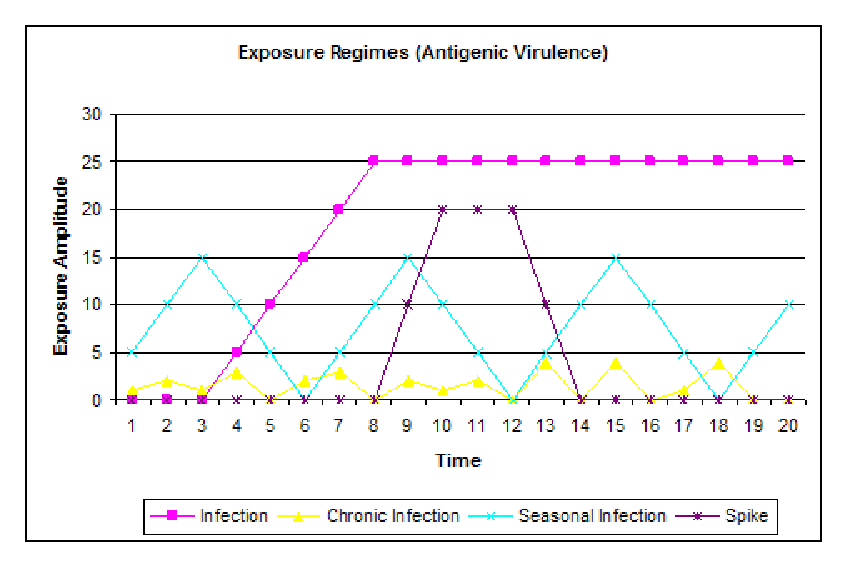
\includegraphics[scale=0.70]{Cells/exposures-virulence}
	\caption{Example exposure regimes demonstrating some archetypical pathogen virulence behaviours.}
	\label{pic:cells:virulence}
\end{figure}

% antigenic virulence
The relationship between a pathogen exposure regime and an immune systems response effort is interesting. For a single exposure event, virulence defined the amount of tissue damage an antigen may cause on a host, therefore it may provide a conception of the amount of specificity refinement (effort) required of an immune system for the exposure. An exposure regime provides a way of crisply defining \emph{antigenic virulence} (distinct from single exposure virulence) as a function of exposures through time. The amount of specificity refinement by the system for the antigen (response effort) is proportional to the exposure frequency and exposure amplitude (exposure regime). Antigenic virulence (and exposure regimes) may be expressed as an exposure amplitude graph against time. From this level of abstraction, one may give example exposure regimes as archetypical pathogen virulence strategies with which to subject an immune system (see Figure~\ref{pic:cells:virulence}). In addition to static antigenic virulence, it is possible for virulence to vary through time. The variance in virulence may be system-dependant such that virulence changes in response to the internal actions of the immune system such as in the case of an adversarial antigen (pathogen). 
% implications to the system
For a multiple exposure event, the system is primarily concerned with devising a response to each exposure and ultimately using past exposures to anticipate the resources needed for future exposures. This exposure model supersedes the single exposure event, as in the case of a single exposure, all resources of the repertoire are allocated to the specific concerns of the antigen (as there are no other antigens). The learning that the system may achieve within the context of a single exposure may be limited, as a broader exposure regime may define how often the exposures arrive to the system. The exposure regime may impose a quantity and specificity capability constraints for a single exposure, meaning that a finite amount of specificity learning and/or quantity learning may be achieved for a single exposure event. The system must learn to anticipate (1) the required specificity of future exposures, and (2) the required quantity of future exposures, both in the face of non-exposure events. 

% plots
\begin{figure}[htp]
	\subfloat[Single Exposure Model.]{
	\label{fig:cells:exposures:flowdiagram:single} %% label 
	\begin{minipage}[t]{0.50\textwidth}
		\centering 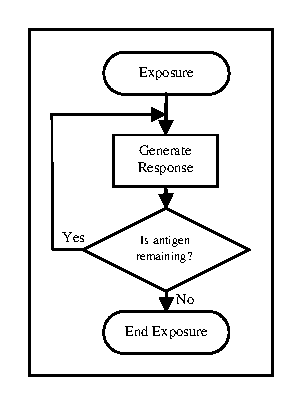
\includegraphics{Cells/exposures-single-model}
	\end{minipage}}%
	\hfill
	\subfloat[Multiple Exposure Model.]{
	\label{fig:cells:exposures:flowdiagram:multiple} %% label 
	\begin{minipage}[t]{0.50\textwidth}
		\centering 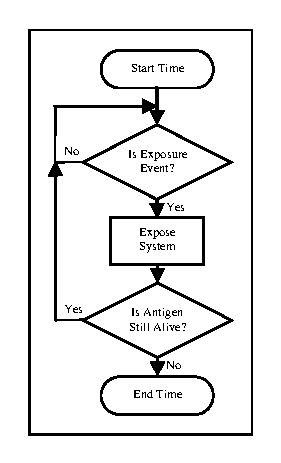
\includegraphics{Cells/exposures-multiple-model}
	\end{minipage}}\\
	% end
	\caption{Flow diagram of the single and multiple exposure models.}
	\label{fig:cells:exposures:flowdiagram} %% label for entire figure
\end{figure}

The exposure regime (frequency and amplitude) define the antigenic virulence and the systems required specificity. Repeated application of blind clonal selection facilitates improvement of a repertoire specificity for the antigen, and for a system that enters stasis during periods of non-stimulation (information acquired by the repertoire does not degrade), the density of information (clonal convergence and/or clonal densities) may define the quantity or scope of information required for the regime. Therefore, a repeated single selection on a relatively \naive\ repertoire fosters a model that matches the virulence of the antigenic exposure regime. For a repertoire with decoupled maintenance of cells and triggered adaptation, an explicit memory mechanism is required that retains acquired information proportional to the frequency of its exposure and complexity. For lower-complexity information, a more efficient strategy may be to generalise or re-acquired as need. 


%
% Multiple Antigen
%
\subsubsection{Multiple Antigen Model}
The natural extension of multiple antigen exposures is to subject an immune system to multiple concurrent exposure regimes. Each regime is expressed by a distinct \emph{antigenic type} or variety. Antigen types differ in their composition (surface features) such that the immune system has to acquire different immunity characteristics for each. In addition to the varied immunity characteristics, each antigen type has its own exposure regime, thus in the context of an immune system, the regime elicits a distinct response effort. The aggregation of multiple antigen types is an aggregation of multiple antigen exposure regimes to a given immune system that may collectively be referred to as the exposure or \emph{antigenic environment}. In responding to one given antigen, the repertoire may acquire a level of immunity (specificity) to another different and distinct pathogen type. This effect is called cross-reactivity of the immune response and may be conceptualised as reuse and generalisation of acquired information. One may consider an immune system to be exposed to the multiple different exposure regimes shown in Figure~\ref{pic:cells:virulence}. In this example, the system is exposed to all four different antigen with varied amplitudes at the discrete time of $t=11$. This may be referred to a \emph{concurrent antigen exposure}. Exposure concurrency requires that the repertoire is (1) large enough (with regard to the quantity of lymphocytes), and (2) diverse enough (with regard to lymphocyte specificity) to address multiple pathogen types at the same time. It is expected that the efficiency of the system will be reduced in such a situation, as resources are allocated proportional to the relative virulence of each antigen type. This effect highlights the requirement of the system to be able to not only respond to multiple antigen types at the same time, but to integrate the results of the concurrent responses (expanded clones and shifted the repertoire specificities).

Unlike the previous two models that were able to allocate all the resources of the repertoire to a single exposure of antigen information, multiple antigens requires a proportional allocation of resources to each antigen and its exposure regime. The proportionality of the response and allocation of repertoire resources is defined by the relative antigenic virulence to other antigen in its environment. The previous concerns of optimising specificity, quantity, and the anticipation of these values may be reduced to the systems adaptation of information densities toward exposure regimes. The density is representative of the learned (aggregated from experience) cell quantity (clone size) and specificity in the repertoire which facilitates anticipatory responses. Each cell has an affinity response surface (affinity landscape) for each pathogen it has been (and may be) exposed to. The clonal densities are acquired from the antigenic virulence which is defined as the amplitude and severity of exposures (amount of learning opportunity offered) to the system through time. This model provides the pinnacle in environments for clonal selection at the cellular level and a complement for the quintessential clonal selection framework.

%
% Exposure Models and Control
%
\subsubsection{Exposure Models and Control}
% general
The environment and the system may be considered two interdependent and required components of which neither is meaningful in isolation. In modelling these two components, one may consider the variable (configurable) aspects of each of which may or may not be within the control of a given simulation. 
% control
An intuitive example is to consider the environment (and therefore all aspects of antigen exposure) as outside of the scope of control, and all aspects of the system as inside of the scope of control. In this example the system must do all it can to cope with the specific properties of the exposures it is subjected to by the environment. The system must operate with finite resource, thus constraints are imposed on the control over aspects the system. This example may be extended further to consider that the evolution of antigen (pathogen) is influenced by the existence and evolution of the host system and that this relationship is reciprocal (co-evolution). Therefore, the system has influence (implicit influence via evolution) over aspects of antigen exposure over longer periods of time, and the antigen has influence (implicit influence via evolution) over aspects of the systems response over the same longer periods of time. This example may be generalised such that aspects of control are variable across both the environment and the system. 

\begin{figure}[ht]
	\centering
	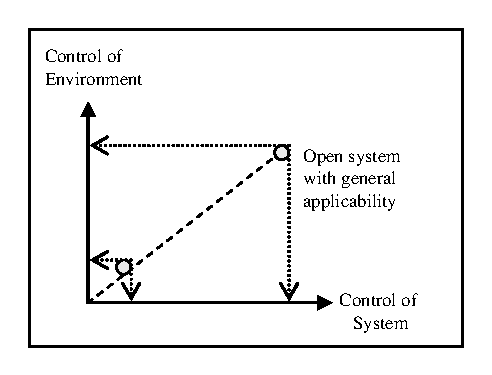
\includegraphics[scale=0.85]{Cells/exposures-tradeoff}
	\caption{Depiction of the trade-off between control of the environment and control of the system.}
	\label{pic:cells:tradeoff}
\end{figure}

% modelling control
In modelling \emph{environment} and \emph{system} and their \emph{interactions}, control may be exhibited over all aspects of both sides of the interaction. It is important to consider the influence for control or lack there of (constraints on control) on a system and its environment as it provides insight into the mapping of domain properties. A constraint may be considered the prior selection of a configuration parameter of a system or environment. The fixing of a configuration parameter in the environment influences the suitability of other unconstrained (controlled) parameters in the interaction, and the influence is likely to be complementary (such that fixing an aspect of the environment strongly influences the suitability of related parameters of the system and vice versa). This point highlights the symmetry of constraint between \emph{systems} and \emph{environments}, and the need to specialise a given system for the constraints of a given environment in which it is to be deployed (mapped problem domain).

%
% Colour Space Domain
%
\subsection{Colour-Space Domain}
\label{subsec:cells:paradigm:colourspace}
In his book detailing the Cognitive Theory of acquired immunity, Cohen used an example of cellular degeneracy in the retina as an analogy for the degeneracy of cell-bound receptors in the immune system \cite{Cohen2001a}. Cohen described how individual cells in the retina have limited capability, responding to constrained wavelengths of light, although from these specific degenerate detectors higher-level information such as a coherent image can be perceived through aggregation. The Self-Organizing Map (SOM) is a competitive and unsupervised learning algorithm that is renowned for its feature extraction and dimensionality reduction capabilities (see Section~\ref{subsec:cs:related:competitive}). In his doctoral work, Honkela used a colour domain (red-green-blue or RGB), and a dataset of known colours in that domain \cite{Honkela1997} (page 14-18). The learning and ordering of the domain of RGB colours based on the dataset was used as an intuitive example of the topological preserving properties of the SOM algorithm. Although Honkela may not have been the first to employ this example domain to the SOM, it has become a canonical example domain.\footnote{There are many applet and tutorial web sites on the Internet that use this example to demonstrate the SOM, the listing of which is not necessary.} Inspired by the simplicity and suitability of the colour domain to qualitatively (visually), and quantifiably (numerical measures) demonstrate the properties of the SOM, this section defines a \emph{colour-space} domain from which a suite of test problem instances may be drawn to investigate clonal selection. Inspired by Cohen's analogy to the retina, colour-space is named for the relationship to the shape-space formalism, and is supported by proven use of the same principle for a related Competitive Learning paradigm.

%
% Contrived Domain
%
\subsubsection{Domain Definition}
The domain does not provide a framework for investigating the so-called colour space theory, which refers to the study of colour models used in display and printer systems. Nor is the intention of the defined test domain for the study of colour theory, the investigation of colour segregation, colour recognition, palette compression, or colour clustering (or any other practical colour-based application domain). Given what the intentions are not, this section outlines a series of general goals for designing a test domain for adaptive systems, followed by the definition of a simple colour-space domain that meets these goals. The ambition is to contrive a domain from which trivial problem instances can be drawn to preliminary assess specific properties of adaptive models. These models may be engaged in processes that equate to pattern recognition and optimisation, and may involved the evaluation of broad characteristics such as learning, memory, and adaptation. See Table~\ref{tab:cells:colourspace:goals} for a list of the general design goals (requirements) for a problem domain suitable for this purpose.

\begin{table}[ht]
	\centering\small
		\begin{tabularx}{\textwidth}{lX}
		\toprule
		\textbf{G\#} & \textbf{Goal} \\ 
		\toprule
		G1 & The domain must provide a numerical and/or combinatorial basis that may be manipulated meaningfully by operators. \\ 
		\midrule
		G2 & The response surface must be correlated such that localised regions in the response surface have a gradient. \\ 
		\midrule
		G3 & The domain must be suitable for optimisation tasks.  \\ 
		\midrule
		G4 & The domain must be suitable for pattern recognition tasks. \\ 
		\midrule
		G5 & The domain must be parameterised such that the relative complexity may be meaningfully adjusted. \\ 
		\midrule
		G6 & The domain must be easily and meaningfully visualised both online (dynamically) and off-line (end of run). \\ 
		\midrule
		G7 & The domain must be easy to understand, easy to implement, and easy to analyse. \\ 
		\midrule
		G8 & The properties of the domain (e.g. the response surface or visualisation) should facilitate rather than mask model behaviours being investigated. \\ 
		\bottomrule
		\end{tabularx}	
	\caption{List of goals for a colour-space domain.}
	\label{tab:cells:colourspace:goals}
\end{table}

The colour-space domain formalism meets the list of goals proposed in Table~\ref{tab:cells:colourspace:goals}. The formalism is comprised of a series of terms to describe the characteristics of a colour space domain. The characteristics identified include the environment: the cardinality, the representation, and the mapping function (see Table~\ref{tab:cells:colourspace:definition} for their definition and summary).

\begin{table}[ht]
	\centering\small
		\begin{tabularx}{\textwidth}{llX}
		\toprule
		\textbf{Term} & \textbf{Name} & \textbf{Summary} \\ 
		\toprule
		$E$ & Environment & The search space (colour space) which defines the scope of feasible coordinates defined by its dimensionality (1-$n$), a boundary (limits of each dimension), and cardinality ($C$). \\ 
		\midrule
		$R$ & Representation & An encoding used and manipulated by adaptive models. It may be binary, integer, real, and may or may not directly represent a coordinate in the colour space ($E$). \\ 
		\midrule
		$M$ & Mapping Function & Converts a given representation ($R$) into a coordinate in the colour space ($E$). If the representation used matches the coordinate system of the environment, then the mapping function returns an unchanged coordinate. \\ 
		\midrule
		$C$ & Cardinality & The number of discrete points in the domain, and ideally (given display capabilities) the number of colours available for visualisation. \\ 
		\midrule
		$I$ & Intention & The goal of a system within the domain, a task or action it is to perform or achieve. This is a cover-all term for something to do in a defined colour-space. \\ 
		\bottomrule
		\end{tabularx}	
	\caption{Summary of terms for the colour space domain formalism.}
	\label{tab:cells:colourspace:definition}
\end{table}

The environment ($E$) is an $n$-dimensional hypercube (for visualisation purposes perhaps limited to 1-3 dimensions), where each dimension represents a different colour axis. The intention is that a distinct coordinate in a given environment (colour space) represent a distinct colour. For example, a monochrome (one-colour) environment would be implemented as a one-dimensional space (line) perhaps a gradient of white to black. An RGB colour space would be implemented as a three-dimensional (cube) environment. An environment is a volume of feasible discrete points, and the cardinality ($C$) defines the number of points in that volume. The granularity of each dimension in the environment also determines the number of colours, thus cardinality may be thought of as the palette of the environment. Further, the palette analogy may be exploited further in defining standard cardinalities, such as those common palettes that are used in computer display systems (for example, 8-bit colour ($2^{8}$) with a pallet of 256 colours). The coordinate-based representation ($R$) may be used directly by an adaptive system. Alternatively a symbolic or sub-symbolic representation may be used (such as bit-strings), which require a mapping function ($M$) to transform representation into a given environments coordinate system. 
The task of an adaptive system is called an intention ($I$), examples may include the optimisation of a randomly initialised system to a set of pre-selected points, or the adaptation of a system to a defined region within the environment.

One may measure the Euclidean distance between points in the colour space as a quantitative measure of difference. Distances measures may not be limited to Euclidean distance, for example Manhattan distance (and many others, see \cite{Kohonen2001} pages 17-29) may be used in the colour space. Distance measures may be augmented with coordinate radii such that a point of interest in the space may represent a collective of points in its vicinity. Such regions may be defined as hyper-cubes or spheres, and may have a distance-based falloff such as linear, Gaussian or exponential. These distances and coordinate neighbourhoods are also qualitatively meaningful. Following a line (for example in a monochrome or RGB) in colour space shows a transition through intermediate colour coordinates (colours). These intermediate colours are quantifiably distinct (numerical coordinates), and qualitatively different (assuming the colour transition can be detected by the human eye). This correlation is also useful for visualisation: agents representing coordinates in the colour space may be implemented, which may permit qualitative measures and observations of system behaviour. 

%
% Illustrative Examples
%
\subsubsection{Illustrative Examples}
This section proposes an \emph{optimisation}, \emph{pattern recognition}, and \emph{classification} examples of Colour Space Problems that adaptive systems that may be employed or extended to investigate adaptive models. 

\begin{itemize}
	\item \emph{Optimisation}: Involving the pre-selection of a coordinate in the space that is withheld from the adaptive system, and defining a cost function as a distance measure to the given coordinate. For example if a space was defined as an 8-bit one-dimensional domain (0-255), a goal coordinate of 127, and an Euclidean distance measure employed as a cost function, then the shape of the response surface would be a triangle with the apex at the selected coordinate. 
	\item \emph{Pattern Recognition}: The optimisation domain may be generalised with a set of goal coordinates (Colour Space Patterns) to which a given system is exposed. The intention of the system for this problem is to optimise (optimally match) the set of patterns, where the order of exposure of the patterns to the system is also withheld from the system.
	\item \emph{Classification}: A classification task may be defined as an extension of the pattern recognition problem with the addition of categorical information. A geometry can be defined within the colour space and class labels can be assigned to the resulting concave regions. In addition to distance-based feedback, the system may be provided with corrective categorical based feedback, relaxing the optimisation of the goal coordinates to that of accuracy of predicting pattern classes.
\end{itemize}


%
% Criticisms and Limitations
%
\subsubsection{Criticisms and Limitations}
This section addresses the important consideration's of the limitations of the formulated problem domain, as follows:

\begin{enumerate}
	\item \emph{Triviality}: The domain and resultant problem definitions are primitive. The problem instances are likely easily solved rapidly by standard deterministic techniques, and even by \naive\ approaches such as enumeration and random search.
	\item \emph{Transferability}: The results achieved on one or a set of derived problem instances are very likely to be not transferable to problem domains of interest (difficult, real-world). Conclusions regarding model performance are limited to the instances on which they are tested, and perhaps related trivial domains.
	\item \emph{Difficulty}: Although superficiality they appear trivial, there is no innate sense of the absolute or relative difficulty of the derived problem definitions.
	\item \emph{Visibility}: For high-cardinality domains (such as those at or above 24-bit or 32-bit RGB) the human eye cannot detect colour differences between coordinates within close proximity.
	\item \emph{Novelty}: The colour space domain and derived problem instances are not novel, they are generalisations and simplifications of existent test domains and benchmark problems.
\end{enumerate}

It is prudent not to rebut these criticisms, but to acknowledge them as limitations (designed or otherwise) of the domain and framework that it provides. The domain and resultant problem instances are intended to be trivial (easy to solve) such that the attention remain on the model under study. The performance of a given model is not intended to be transferable, what is expected to be transferable are the general functional behaviours that the domain assists in isolating and assessing. The relative difficulty of problem instances may be determined by baseline strategies. Comparable relative and absolute difficulty may be defined using the tools of probability, statistical mechanics, and additional (suitable) mathematical apparatus. The visual distinctiveness of close-proximity coordinates in high-cardinality spaces may be exaggerated where appropriate. For example, a dynamically normalised colour scale may be allocated to coordinates of interest. Finally, novelty is not claimed, rather the domain is a \emph{consistent reformulation} of classical optimisation and pattern recognition benchmark domains.

%
% Realised Cellular Paradigm
%
\section{Realised Cellular Paradigm}
\label{sec:cells:realised}
This section provides a realisation of the concerns of the abstract \emph{Cellular Clonal Selection Paradigm} presented in Section~\ref{sec:cells:paradigm}. This includes general definitions of a standardised problem domain in the Antigenic Exposure Problem as a specialisation in colour space, and the Cellular Clonal Selection Algorithm that provides a basis for investigation into elaborated cell interaction schemes. A series of cell-based measures are presented for assessing cellular algorithms on instances of Antigen Exposure Problems that provide quantitative indicators regarding the concerns of information acquisition and application. Collectively, this section provides a basis for the implementation and exploratory empirical investigation into the Cellular Clonal Selection Paradigm, as well as a bridge between the biology (Section~\ref{sec:cs:theory}) existing approaches (Section~\ref{sec:cs:algorithms}), and the abstract clonal selection and antigenic exposure models (Section~\ref{sec:cells:paradigm}).


%
% Antigenic Exposures
%
\subsection{Antigenic Exposures}
\label{sec:cells:realised:exposures}
This section considers the realisation of the specialisations of the exposure paradigm outlined in Section~\ref{subsec:cells:paradigm:antigenicexposures} as a basis for empirical investigation and ultimate application of cellular models to problem domains. This realisation includes the definition of general antigenic exposure problem with exposure regimes, and a specialisation to the colour space domain.

%
% Antigenic Exposure Problem 
%
\subsubsection{Antigenic Exposure Problem}
% general nomenclature
For the purposes of discussing exposure, a cellular clonal selection algorithm may be reduced to its information content, distinct from the specific clonal selection processes operating upon that information. Specifically, a cellular algorithm may be considered a population or repertoire ($T$, that stands for `tissue' which will be made apparent in proceeding chapter) of discrete cells ($C$), as follows: $T = \{C_1, C_2, C_3 \ldots, C_n\}$. Therefore an \emph{Antigenic Exposure Problem (AEP)} is defined as the discrete interaction with a $T$, with a set ($I$, which stands for `infection') of antigen ($A$) at the same level of abstraction, as follows $I = \{A_1, A_2, A_3 \ldots, A_n\}$. An antigen is comprised of sub-antigenic information referred to as determinants ($D$), such that $A = \{D_1, D_2, D_3 \ldots, D_n\}$. 

\begin{algorithm}[ht]	
	\SetLine
	
	\SetKwFunction{StopCondition}{StopCondition}	
	\SetKwFunction{CreateRandomAntigen}{CreateRandomAntigen}
	\SetKwFunction{Exposure}{Exposure}
	
	\SetKwData{Infection}{I}
	\SetKwData{Tissue}{T}
	
	\KwIn{\Tissue, $N_{determinants}$ $N_{antigen}$}
	\KwOut{$T_{rs}$}
	
	% prepare
	\Infection $\leftarrow$ 0\;
  \For{i$\leftarrow$0 \KwTo $N_{antigen}$}
  {
  	$A_i \leftarrow$ \CreateRandomAntigen{$N_{determinants}$}\; 
  	\Infection $\leftarrow A_i$\;
  }  
  % exposures
  $T_{rs} \leftarrow$ 0\;
	\While{$\neg$\StopCondition{}}
	{
		$T_{rs} \leftarrow$ \Exposure{\Infection, \Tissue}\;
	} 
	\Return{$T_{rs}$}\;
	\caption{Antigenic Exposure Problem (AEP).}
	\label{alg:cells:realised:exposures:aep}
\end{algorithm}

% algorithm
Algorithm~\ref{alg:cells:realised:exposures:aep} defines a simple antigenic exposure problem, with symmetrical information content for interaction with a given cellular system, where $N_{determinants}$ and $N_{antigen}$ define the number of determinants per antigen and total antigen within the scope of the AEP. The algorithm clearly shows the AEP's in control of the interactions with a given $T$, where discrete interactions are mediated via an $Exposure(I,T)$ operation. The algorithm definition also highlights that from an exposure perspective, the AEP is only concerned with a systems aggregate responses to exposures. The tissue result set denoted as $T_{rs}$ may be considered to represent a cellular algorithm's ($T$) capability to address a given antigen exposure problem ($I$).

%
% Cellular Exposure Regimes
%
\subsubsection{Cellular Exposure Regimes}
The defined antigenic exposure problem delegates the specifics of algorithm-problem interaction to the $Exposure(I,T)$ operation, the behaviour of which may be referred to as a \emph{Cellular Exposure Regime (CER)}. For example, the information content of the problem may be exposed to a system (1) consistently in the same order, (2) in a randomised order, or (3) in some biased manner resulting in an asymmetric perspective of such information content. Referring to such interactions as an exposure regimes also highlights the important point that the cellular algorithm is considered a passive information processing system that responds to the active exposure of antigenic stimuli. Therefore, depending on the specific problem domain, the concerns of exposure, re-exposure, and multiple exposures (from Section~\ref{subsec:cells:paradigm:antigenicexposures}) may or may not be within the scope of control of the system. Algorithm~\ref{alg:cells:realisation:exposure:aep:cer} provides an example of a regular and consistent exposure regime $Exposure(I,T)$ operation where a system is exposed and must respond to the scope of the AEP each $I$ exposure called an epoch. The example also delegates the responsibility of specific cell interaction (selection and response) to the cellular clonal selection algorithm in the $Exposure(A,T)$ operation. This operation encapsulates the scope of concerns of algorithms in the cellular paradigm.

\begin{algorithm}[ht]	
	\SetLine
	\SetKwFunction{Exposure}{Exposure}	
	\SetKwData{Infection}{I}
	\SetKwData{Tissue}{T}
	
	\KwIn{\Infection, \Tissue}
	\KwOut{$T_{rs}$}
	
  % exposures
  $T_{rs} \leftarrow$0\;
	\ForEach{$A_i \in $ \Infection}
	{		
		$C_{i} \leftarrow$ \Exposure{$A_i$, \Tissue}\;
		$T_{rs} \leftarrow C_{i}$\;
	} 
	\Return{$T_{rs}$}\;
	
	\caption{Exposure Function (CER) for the Antigenic Exposure Problem.}
	\label{alg:cells:realisation:exposure:aep:cer}
\end{algorithm}


% the unknowns for a CCSA
The cellular exposure regime represents the uncertainty in the information processing faced by a cellular algorithm, including but not limited to (1) the number of antigen ($N_{antigen}$), (2) the number of determinants for a given antigen ($N_{determinants}$), the diversity of the information in the antigenic environment ($I$), and the ordering of the discrete information exposures defined in the the exposure regime itself (CER). Finally, discrete cellular interactions with antigen and determinants may not yield specific information, rather a general indication. For example from an abstract point of view an $Exposure(A, C)$ or $Exposure(D, C)$ may result in a relative indication of fit or suitability (affinity or avidity) rather than absolute cost. This is motivated by the pre-committed, iterative, and trial-based (selectionist) strategy reduced from the clonal selection theory.

%
% Antigen Colour Space Problem
%
\subsubsection{Antigen Colour Space Problem}
% colour space
The antigenic exposure problem may be specialised in the colour space domain as a pattern recognition problem called the \emph{Antigen Colour Space Problem (ACSP)}. The problem is defined as a set of Colour Space Patterns (CSP) each of which is defined as a colour comprised of three 64-bit colour components. The set of patterns are generated as a set of random binary strings ($A\prime = \{0,1\}^{L}$, where $L=(3\times64)$) and decoded using the Gray Code method for each colour component (Equation~\ref{eq:cells:realised:graycode}, where $\bigoplus $ denotes addition modulo two) to a three dimensional colour vector $A = [0,1]^{3}$. Cellular solutions ($C$) to each antigen colour space pattern ($A$) are 192-bit binary strings that decoded to 3-dimensional colour vectors using Gray Code. The affinity (avidity) function for a decoded cell, the $Exposure(A, C)$ is defined as the Euclidean distance between the two vectors (Equation~\ref{eq:cells:realised:euclidean}).

% Gray Code
\begin{equation}
	GrayCode(A\prime) = \frac{1}{2^{64}-1} \left(\sum_{j=0}^{64-1} \left(\bigoplus_{k=1}^{64-j}A\prime(i-1) 64+k\right) 2^j\right)
	\label{eq:cells:realised:graycode}
\end{equation}

% Euclidean Distance
\begin{equation}
	EuclideanDistance(A, C) = \sqrt{\sum_{i=1}^n  \left(A_i - C_i\right)^2}
	\label{eq:cells:realised:euclidean}
\end{equation}

% minimum
This mapping of the colour space problem onto the antigenic exposure problem highlights the important point of the minimal cases of the problem, specifically: (1) minimum determinant, and (2) minimum antigen. From an abstract perspective, a cell matches onto one determinant, from an antigen of multiple determinants. Therefore, from a system perspective a one-to-one relationship exists between a given cell and its cognate antigen mediated via the specific sub-feature (antigenic determinant). A \emph{Minimum Determinant Antigenic Exposure Problem (MDAEP)} may be defined where each antigen is comprised of a single determinant ($N_{determinants}=1, \forall A \in I$). This case forces such a one-to-one relationship at the cost of the exclusion of the cross-reactivity of cells. In the same manner, the number of antigen in the set may be minimised ($N_{antigen}=1$) to define a \emph{Minimum Antigenic Exposure Problem (MAEP)} where a given system $T$ is assessed based on its capability with a single antigen with a single determinant. This minimal case (single or multiple exposures of a single determinant), provides a minimal context in which to consider fundamental behaviours of cellular algorithms and their extensions.

%
% Cellular Clonal Selection
%
\subsection{Cellular Clonal Selection}
\label{sec:cells:realised:algorithms}
This section considers the realisation of specialisations of quintessential clonal selection outlined in Section~\ref{subsec:cells:paradigm:clonalselection} as a basis for empirical investigation and ultimate application of cellular models to problem domains. This realisation includes the definition of a general cellular clonal selection algorithm as a homologue to CLONALG, and a replacement based extension.

%
% Cellular Clonal Selection Algorithm
%
\subsubsection{Cellular Clonal Selection Algorithm}
% general
A \emph{Cellular Clonal Selection Algorithm (CCSA)} is defined as the application of the computational properties of the clonal selection theory constrained by the concerns of the theory at the cellular-level. These constraints include but are not limited to (1) the interaction with antigen via their determinants, (2) the embodiment of information in a self-contained repertoire of discrete cells, and (3) the cellular response to active antigenic exposures. The extent of the taxonomy of clonal selection algorithms reviewed in Section~\ref{sec:cs:algorithms} may be considered to reside in the cellular level (within the scope of the Cellular Clonal Selection Paradigm).
% abstraction
This section considers an abstraction of cellular clonal selection algorithms in the context the concerns considered in quintessential Clonal Selection in Section~\ref{subsec:cells:paradigm:clonalselection}. The Antigen Exposure Problem defined a cellular system in terms of its information content, where the problem is the active concern and the cellular system is passive until exposed with stimuli to which it reflexively responds. The scope of the concerns of cellular clonal selection algorithms are the management of information within the repertoire, and in particular the management of information under the discrete exposures of an AEP.

\begin{algorithm}[ht]
  \SetLine
  \SetKwData{T}{T}
  \SetKwFunction{CreateCell}{CreateCell}   
  \KwIn{$N_{cells}$}		
  \KwOut{\T}  
  
	\T $\leftarrow$ 0\;	
	\For{i$\leftarrow$0 \KwTo $N_{cells}$}
	{
		$C_i \leftarrow$ \CreateCell{}\;
		\T $\leftarrow C_i$\;
	}
	\Return{\T}\;
	\caption{Initialisation Function for the Cellular Clonal Selection.}
	\label{alg:cells:realisation:algorithms:ccsa:init}
\end{algorithm}

% algorithm
Algorithm~\ref{alg:cells:realisation:algorithms:ccsa:init} defines an initialisation operation for a the Cellular Clonal Selection Algorithm, where the $CreateCell()$ may be specialised to create random cells with a representation appropriate for the specific problem domain (192-bit binary strings in the case of the ACSP). Algorithm~\ref{alg:cells:realisation:algorithms:ccsa:exposure} defines the $Exposure(A, T)$ operation for the CCSA that provides a generalisation of the CLONALG, BCA, AIRS, and IA family of the reviewed clonal selection taxonomy. Specifically, the algorithm responds to antigen exposures by assessing the extent of the repertoire and selecting a subset ($N_{selected}$) to comprise a response. Each cell in the selected set creates a set of clones ($N_{clones}$) with mutations ($P_{mutation}$) that are assessed against the antigen and compete with the progenitor of the selected set for a position in the repertoire. This generalisation which strongly resembles CLONALG, implicitly manages the memory cell set and explicitly returns a best matching cell ($GetBestMatchingCell(T)$) for each exposure as the most suitable response within the scope of the repertoire. Importantly, the CCSA provides the flexibility to assume a variety of configurations, specialisations (such as the CSA taxonomy), as well as the extensions considered in this chapter.

% CCSA
\begin{algorithm}[ht]
  \SetLine	
  
  \SetKwData{Antigen}{A}
	\SetKwData{Tissue}{T}
  
	\SetKwFunction{Clone}{Clone}
	\SetKwFunction{Mutate}{Mutate}
	\SetKwFunction{Select}{Select}
	\SetKwFunction{Expose}{Expose}
	\SetKwFunction{GetBestMatchingCell}{GetBestMatchingCell}
	\SetKwFunction{Remove}{Remove}
	\SetKwFunction{Add}{Add}
	
  \KwIn{\Antigen, \Tissue, $N_{selected}$, $N_{clones}$, $P_{mutation}$}
	\KwOut{$T_{rs}$} 
	
 	% exposure
 	$T_{rs} \leftarrow0$\;
 	\ForEach{$C_i$ $\in$ \Tissue}
 	{
 		\Expose{\Antigen, $C_i$}\;
 	}
	% selection
	$T_{selected} \leftarrow$ \Select{\Tissue, $N_{selected}$}\;
	% cloning and competition
	\ForEach{$C_i$ $\in$ $T_{selected}$}
	{
		% clone and mutate
		$T_{clones} \leftarrow 0$\;
		\For{i$\leftarrow$0 \KwTo $N_{clones}$}
		{
			${C\prime}_i \leftarrow$ \Clone{$C_i$}\;
			${C\prime}_i \leftarrow$ \Mutate{${C\prime}_i$, $P_{mutation}$}\;
			$T_{clones} \leftarrow {C\prime}_i$\;
		}
		% expose clones
		\Expose{\Antigen, $T_{clones}$}\;
		% select the set
		${T\prime}_{clones} \leftarrow$ \Select{$T_{clones}$, $N_{selected}$}\;
		% competition for position
		\For{i$\leftarrow$0 \KwTo $N_{selected}$}
		{
			$C_{selected} \leftarrow {T_{selected}}_i$\;
			$C_{clone} \leftarrow {{T\prime}_{clones}}_i$\;
			\If{$C_{clone}$.score $\leq C_{selected}$.score}
			{
				\Tissue.\Remove{$C_{selected}$}\;
				\Tissue.\Add{$C_{clone}$}\;
			}
		}
	}
	% select bmu
	$T_{rs} \leftarrow$ \GetBestMatchingCell{\Tissue}\;
	\Return{$T_{rs}$}
	\caption{Exposure Function for the Cellular Clonal Selection.}
	\label{alg:cells:realisation:algorithms:ccsa:exposure}
\end{algorithm}

% minimal
The CCSA may be reduced to a minimal configuration to provide a complement to the Minimal Antigenic Exposure Problem called the \emph{Minimal Cellular Clonal Selection Algorithm (MCCSA)}. This minimal configuration under the MAEP provides a realisation of of the ES$(1+1)$ algorithm and connection with mutation based hill climbers made in Section~\ref{sec:cs:related}. For example, ES$(1+1)$ would be defined by the configuration: $N_{cells}=1$, $N_{selected}=1$, $N_{clones}=1$, and $P_{mutation}=\frac{1}{L}$.

%
% Replacement Cellular Clonal Selection Algorithm
%
\subsubsection{Replacement Cellular Clonal Selection Algorithm}
An expected effect with the Cellular Clonal Selection Algorithm is that it results in the iterative adaptation of specialised and independent cells. This is expected (1) because it was observed in CLONALG with regard to a niching-like effect, and (2) because CCSA and CLONAL resemble a parallel mutation based hill climber. The \emph{Replacement Cellular Clonal Selection Algorithm (RCCSA)} defined in Algorithm~\ref{alg:cells:realisation:algorithms:rccsa:exposure} is an extension of the CCSA where all clones created for an exposures are aggregated into a clonal set, which then competes with the cells in the repertoire on a per-cell basis for a limited position in the repertoire. This `clonal set-repertoire competition' is intended to provide more opportunity for per-exposure resource allocation, by allowing clones to compete and potentially displace repertoire members that may or may not be the clonal progenitor (progenitor of clones), clonal siblings (same progenitor), or exposure clonal siblings (same exposure). This competition is promoted firstly through a cell-to-cell distance assessment that simulates the competition the cells face during selection by antigen where similar cells compete for the same antigenic patterns, and in the affinity comparison that selects those cells that respond better to the specific antigen to which the system has been exposed. This competition mechanism decouples intra-repertoire competition for survival in the integration of clones from the antigenic-based selection that resulted in the creation of the clones. Such decoupling may be exploited in the integration of cells with varied origins. 

\begin{algorithm}[ht]
  \SetLine
  \SetKwData{Antigen}{A}
	\SetKwData{Tissue}{T}

	\SetKwFunction{Clone}{Clone}
	\SetKwFunction{Mutate}{Mutate}
	\SetKwFunction{Select}{Select}
	\SetKwFunction{Expose}{Expose}  
  \SetKwFunction{Remove}{Remove}
	\SetKwFunction{Add}{Add}
	\SetKwFunction{Distance}{Distance}
	\SetKwFunction{GetBestMatchingCell}{GetBestMatchingCell}
	
  \KwIn{\Antigen, \Tissue, $N_{selected}$, $N_{clones}$, $P_{mutation}$}
	\KwOut{$T_{rs}$} 	
	
 	% exposure
 	$T_{rs} \leftarrow$0\;
 	\ForEach{$C_i \in$ \Tissue}
 	{
 		\Expose{\Antigen, $C_i$}\;
 	}
	% selection
	$T_{selected} \leftarrow$ \Select{$T$, $N_{selected}$}\;
	$T_{clones} \leftarrow$0\;	
	% cloning and mutation
	\ForEach{$C_i \in T_{selected}$}
	{
		% clone and mutate
		\For{i$\leftarrow$0 \KwTo $N_{clones}$}
		{
			${C\prime}_i \leftarrow$ \Clone{$C_i$}\;
			${C\prime}_i \leftarrow$ \Mutate{${C\prime}_i$, $P_{mutation}$}\;
			$T_{clones} \leftarrow {C\prime}_i$\;
		}
	}
	% expose clones
	\Expose{\Antigen, $T_{clones}$}\;		
	% competition for position
	\For{$C_{clone}$ \KwTo $N_{clones}$}
	{
		% locate most similar
		$C_{selected} \leftarrow 0$\;
		\ForEach{$C_i \in T$}
		{			
			\If{\Distance{$C_{clone}$, $C_i$} $<$ \Distance{$C_{clone}$, $C_{selected}$}}
			{
				$C_{selected} \leftarrow C_i$\;
			}
		}
		% compete		
		\If{$C_{clone}$.score $\leq C_{selected}$.score}
		{
			\Tissue.\Remove{$C_{selected}$}\;
			\Tissue.\Add{$C_{clone}$}\;
		}
	}	
	% select bmu
	$T_{rs} \leftarrow$ \GetBestMatchingCell{\Tissue}\;
	\Return{$T_{rs}$}\;
	
	\caption{Exposure Function for Replacement Cellular Clonal Selection.}
	\label{alg:cells:realisation:algorithms:rccsa:exposure}
\end{algorithm}


%
% Empirical Assessment
%
\subsection{Empirical Assessment}
\label{sec:cells:realised:measures}
This section defines a series of general empirical measures that provide instantaneous information regarding a given CCSA on colour space specialisations of the Antigenic Exposure Problem. An important consideration of these measures in the context of investigation via exploratory experimentation is not their absolute value, but rather their relative change in value with changes to the systems being investigated. Two general classes of measures are considered, (1) error measures that assess the capability of a system in the context of a given problem instance, and (2) diversity measures that consider the general state of the information content within a given system.

%
% Average Cell Error (ACE)
%
\subsubsection{Average Cell Error}
The error of a cell may be assessed as its affinity for a given antigen, and may be assessed using the problem domains specific $Exposure(A, C)$ operation, in this case Euclidean Distance (defined in Equation~\ref{eq:cells:realised:euclidean}). Although not used directly, \emph{Cell Error (CE)} (defined in Equation~\ref{eq:cells:realisation:measure:ce}) provides an error-centric buillding building block for addition error assessments.

% Cell Error
\begin{equation}
	CellError(A,C) = EuclideanDistance(A, C)
	\label{eq:cells:realisation:measure:ce}
\end{equation}

An important application of Cell Error is its calculation for each cell in in the result set ($T_{rs}$) returned from a cellular algorithms $Exposure(I, T)$ operation. The Average Cell Error (ACE) defined in Equation~\ref{eq:cells:realisation:measure:ace} is a problem specific (ACSP) measure for assessing the general capability of a cellular algorithm on an antigenic exposure problem.

% Average Cell Error
\begin{equation}
	AverageCellError(I,T_{rs}) = \frac{1}{I_n} \sum_{i=1}^{{T_{rs}}_n} CellError(A_i, C_i)
	\label{eq:cells:realisation:measure:ace}
\end{equation}

%
% Average Cell Diversity (ACD)
%
\subsubsection{Average Cell Diversity}
A diversity measure of the cellular repertoire provides some indication of the variation in the discrete information stored within the repertoire. Low diversity reflects a homogeneous repertoire, whereas high diversity reflects a heterogeneous set of cells. Given the selected bit string basis of the CCSA, diversity between two cells may be measured as the hamming distance between the cells (see Equation~\ref{eq:cells:realisation:cd}, where Hamming Distance is defined in Equation~\ref{eq:cells:realisation:hamming}, and $\oplus$ denotes exclusive-or (XOR).

% Hamming Distance
\begin{equation}
	HammingDistance(X, Y) = \sum_{i=1}^L \left( X_i \oplus Y_i \right)
	\label{eq:cells:realisation:hamming}
\end{equation}

% Cell Diversity
\begin{equation}
	CellDiversity(C1, C2) = HammingDistance(C1, C2)
	\label{eq:cells:realisation:cd}
\end{equation}

Cell Diversity (CD) can be calculated for each cell in the repertoire against all other cells in the repertoire to provide an indication the average number of bit differences of a given cell to the rest of the cells in the repertories, called the Average Cell Diversity (ACD) defined in Equation~\ref{eq:cells:realisation:acd}.

% Average Cell Diversity
\begin{equation}
	AverageCellDiversity(T) = \frac{1}{T_n}\sum_{i=1}^{T_n} \left(\frac{1}{T_n}\sum_{j=1}^{T_n} CellDiversity(C_i, C_j)\right) 	
	\label{eq:cells:realisation:acd}
\end{equation}


%
% Trends and Behaviours
%
\subsection{Trends and Behaviours}
\label{sec:cells:realised:trends}
This section considers the expected emergent effects and behavioural trends of cellular-based clonal selection algorithms as defined in the specific realisations.

%
% Primitive Behaviour Trends
%
\subsubsection{Primitive Behaviour Trends}
The foundational expectation is that the realised Cellular and Replacement Clonal Selection Algorithm behave much like CLONALG and AIRS. Specifically, that the algorithm will acquire information via selection and adaptation. This section outlines the specific foundational behaviour trends of the algorithms in the context of the pressures and principles of the clonal selection strategy discussed in Section~\ref{subsec:cells:paradigm:clonalselection}.

\begin{enumerate}
	\item \emph{Repertoire Size}: The repertoire size must be sufficiently large to ensure that selection of cells and integration of clones do not result in competition between cells specialised for different antigen. Such competition by an insufficiently sized repertoire is expected to result in unstable behaviour. 
	\item \emph{Selection Size}: The number of clones selected per antigen exposure defines the amount of resources allocated to each antigen under fixed clonal integration. An increase in resource allocation via an increase in selection is expected to result in increased specialisation via the promotion of `concurrent redundant perspectives' of a given antigen. 
	\item \emph{Cloning Size}: The number of clones created per selected cell reflects the amount of computational effort expended on re-sampling modifications on a `known-to-be-good' structure. Therefore an increase in cloning and acceptance of limited high-affinity clones is expected to result in an increased specialisation toward exposed antigen. 
	\item \emph{Replacement Constraints}: Replacement constrained by a clonal progenitor is expected to result in a constrained and specialised hill climbing-like behaviour (MHCA). The relaxation of this constraint such that clonal progeny compete directly with the repertoire is expected to enhance the so-called `concurrent redundant perspectives' to ensure that the maintained multiple perspectives are the most competitive, likely resulting in improved repertoire specialisation.	
\end{enumerate}


%
% Contextual Adaptation Expectations
%
\subsubsection{Contextual Adaptation Expectations}
This section outlines the specific expectations regarding contextual adaptation both with regard to the localisation of activated and responding cells.

\begin{enumerate}
	\item \emph{Localised Activation}: Strong and non-overlapping (specialised for the same antigen) competition by selection is expected to sufficiently localise polyclonal activation and resultant adaptation of the clonal selection strategy (oligoclonal activation).
	\item \emph{Localised Response}: A top-down centralised aggregation of degenerate cells is expected to sufficiently localise a polyclonal response of selected cells under clonal selection.
\end{enumerate}


%
% Paradigm Agenda
%
\subsection{Paradigm Agenda}
\label{sec:cells:realised:agenda}
This section outlines the research agenda regarding the cellular clonal selection paradigm in the remainder of this chapter. Specifically, the agenda is constrained to the investigation of the expectations made regarding primitive behavioural trends of the cellular clonal selection algorithms and the expectations regarding contextual adaptation of cells.

\begin{enumerate}
	\item Investigate the expectations regarding the foundational clonal selection behaviour.
	\item Investigate the expectations regarding contextual adaptation.
	\item Investigate additional mechanism to influence the localisation of adaptation in the clonal selection strategy.	
\end{enumerate}

%
% Cellular Clonal Selection
%
\section{Cellular Clonal Selection}
\label{sec:cells:ccsa}
This section considers three empricial studies of the cellular clonal selection algorithm. Specifically, Section~\ref{sec:cells:ccsa:ccsa} considers the selection and cloning sizes in the Cellular Clonal Selection Algorithm (CCSA), Section~\ref{sec:cells:ccsa:rcsa} considers repertoire resource allocation in CCSA and the Replacement Cellular Clonal Selection Algorithm, and finally Section~\ref{sec:cells:ccsa:dcsa} considers contextual adaptation of symbolic and sub-symbolic degenerate cells under the clonal selection strategy.

%
% Cellular Empirical Study
%
\subsection{Cellular Empirical Study}
\label{sec:cells:ccsa:ccsa}

%
% Aim
%
\subsubsection{Aim}
The aim of this empirical study was to investigate the CCSA as a viable realisation of cellular clonal selection and to assess the expected behaviour of this foundational algorithm with regard to the number of cells selected and the number of clones created under varied antigenic environments. Toward this end, the study had the following goals:

\begin{enumerate}
	\item Assess the repertoire composition and capability of CCSA with small and large selection and clonal sets.
	\item Assess such behaviour under small and large antigenic environments.
\end{enumerate}

%
% Method
%
\subsubsection{Method}

%
% Problems
%
\paragraph{Problems}
The colour space specialisation of the Antigenic Exposure Problem (AEP) was used called the Antigen Colour Space Problem (ACSP). Two variations of the problem were employed ACSP-1 with a single CSP ($N_{antigen}=1$) also referred to as the Minimal Antigen Colour Space Problem, and ACSP-10 with 10 CSP ($N_{antigen}=10$)\footnote{It is important to note that 10 patterns does not represent the expected extent of the approaches capability, rather relative increase over the minimal problem case of one pattern. The scalability of the pattern recognition capability of the investigated approaches is outsides the scope of this thesis, although the approach is expected to be effected by the curse of dimensionality faced with similar pattern recognition systems (see Section~\ref{sec:iidle:function:approximation} for further discussion).}. Both problem instances used the minimal determinant configuration where the scope of the determinant was defined by the extent of each Colour Space Pattern ($N_{determinants}=1$). Colour Space Patterns were randomly generated at the start of each algorithm-problem run. In the case of ACSP-10, CSP were randomly generated and accepted with the constraint that pattern binary strings must have a minimum of a 64-bit Hamming Distance from all other generated patterns for the run. The simple consistent Cellular Exposure Regime (CER) defined in Algorithm~\ref{alg:cells:realisation:exposure:aep:cer} was used to manage the interaction of the problem with the cellular algorithm.

% 
% Algorithms
%
\paragraph{Algorithms}
% algorithms
The study considered four different configurations of the Cellular Clonal Selection Algorithm (defined in Algorithm~\ref{alg:cells:realisation:algorithms:ccsa:exposure}). The CCSA configurations for the ACSP-1 and ACSP-10 are defined in Table~\ref{tab:cells:clonalselection:ccsa:aep1} and Table~\ref{tab:cells:clonalselection:ccsa:aep10} respectively. The mutation rate ($P_{mutation}$) was fixed at $\frac{1}{L}=\frac{1}{192}\approx0.005$ for all algorithm configurations. In addition to the CCSA parameters, the tables also list the derived values for the number of clones created per antigen exposure (\emph{Clones ($A$)}), the number of positions in the repertoire under competition per antigen exposure (\emph{Positions}), and the total number of clones created per infection exposure or epoch (\emph{Clones ($I$)}). For all configurations, the number of cells was set to ensure that selection and cloning did not result in explicit competition for resources between cells specialised for different antigen.

\begin{table}[ht]
	\centering\small
		\begin{tabular}{lllllll}
		\toprule
		\emph{CCSA} & $N_{cells}$ & $N_{selected}$ & $N_{clones}$ & \emph{Clones ($A$)} & \emph{Positions} & \emph{Clones ($I$)} \\ 
		\toprule
		\emph{1+1} & 1 & 1 & 1 & 1 & 1 & 10 \\ 
		\emph{1+N} & 1 & 1 & 10 & 10 & 1 & 100 \\ 
		\emph{N+1} & 10 & 10 & 1 & 10 & 10 & 100 \\ 
		\emph{N+N} & 10 & 2 & 5 & 10 & 2 & 100 \\ 
		\bottomrule
		\end{tabular}
	\caption{Summary of the assessed configuration of CCSA for ACSP-1.}
	\label{tab:cells:clonalselection:ccsa:aep1}
\end{table}

\begin{table}[ht]
	\centering\small
		\begin{tabular}{lllllll}
		\toprule
		\emph{CCSA} & $N_{cells}$ & $N_{selected}$ & $N_{clones}$ & \emph{Clones ($A$)} & \emph{Positions} & \emph{Clones ($I$)} \\ 
		\toprule
		\emph{1+1} & 1 & 1 & 1 & 1 & 1 & 10 \\ 
		\emph{1+N} & 1 & 1 & 10 & 10 & 1 & 100 \\ 
		\emph{N+1} & 100 & 10 & 1 & 10 & 10 & 100 \\ 
		\emph{N+N} & 100 & 2 & 5 & 10 & 2 & 100 \\ 
		\bottomrule
		\end{tabular}
	\caption{Summary of the assessed configuration of CCSA for ACSP-10.}
	\label{tab:cells:clonalselection:ccsa:aep10}
\end{table}

%
% Experiment
%
\paragraph{Experiment}
Each algorithm used the \emph{Maximum Epochs Stop Condition (MESC)} defined in Equation~\ref{eq:cells:stopcondition:epochs} with $MaxEpochs=1000$, where an epoch was defined as the complete exposure of an $I$ to the $T$. The two cellular specific measures defined in Section~\ref{sec:cells:realised:measures} were collected from the state of the system after the triggering of the stop condition. These measures included the Average Cell Error (ACE) and the Average Cell Diversity (ACD). Each algorithm and problem received a new and different random number seed each run. Algorithm-Problem combinations were repeated 30 times.

\begin{equation}	
	StopCondition(Epoch_i) = \left(Epoch_i \geq MaxEpochs\right)
	\label{eq:cells:stopcondition:epochs}
\end{equation}


%
% Results
%
\subsubsection{Results}
% tables
Table~\ref{tab:cells:ccsa:study} provides a summary of results for each algorithm-problem combination including the mean ($\bar{x}$) and standard deviation ($\sigma$) of collected measure values. The non-parametric Mann-Whitney~U statistical test was calculated pair-wise for all algorithms in each problem group. Results are summarised as statistically significant if the null hypothesis that any two given populations in the group are drawn from the same distribution ($H_0: \mu_0 = \mu_1$). Specifically, $H_0$ is rejected if the calculated $p$-value $< \alpha=0.05$, meaning the results are statistically significant at the 5\% level. 
% boxplots
Figures \ref{fig:tissues:ccsa::study0:acd:boxplot} and \ref{fig:tissues:ccsa::study0:ace:boxplot} show the ACD and ACE for all algorithms on ACSP-1 respectively, and figures \ref{fig:tissues:ccsa::study1:acd:boxplot} and \ref{fig:tissues:ccsa::study1:ace:boxplot} show the ACD and ACE for all algorithms on ACSP-10 respectively
% plots
Figure~\ref{fig:cells:ccsa:ccsa:plots} provides an example plot of the $T_{rs}$ returned from the CCSAN+N algorithm on the ACSP-1 and ACSP-10 problems at after the triggering of the stop condition (same configurations as experiment, random seed of 5 and 1 for the problem and algorithm respectively).

% Study 0
\begin{table}[htp]
	\centering\small
		\begin{minipage}{0.50\textwidth}
			\centering
			\begin{tabular}{llllll}
			\toprule
			\textbf{Problem} & \textbf{System} & \multicolumn{2}{c}{\textbf{ACD}} & \multicolumn{2}{c}{\textbf{ACE}}\\
			\midrule
			\emph{ACSP} & \emph{CCSA} & $\bar{x}$ & $\sigma$ & $\bar{x}$ & $\sigma$\\
			\toprule
			ACSP-1 & CCSA1-1 & 0 & 0 & 0.165 & 0.074 \\
			ACSP-1 & CCSA1-N & 0 & 0 & 0.004 & 0.007 \\
			ACSP-1 & CCSAN-1 & 85.267 & 1.104 & 0.041 & 0.027 \\
			ACSP-1 & CCSAN-N & 86.233 & 1.055 & 0.014 & 0.027 \\
			\multicolumn{2}{l}{\emph{Significant}} & True\footnote{False for CCSA1-1 and CCSA1-N} &  & True & \\
			\midrule
			ACSP-10 & CCSA1-1 & 86.363 & 0.808 & 0.161 & 0.037 \\
			ACSP-10 & CCSA1-N & 86.053 & 1.016 & 0.073 & 0.031 \\
			ACSP-10 & CCSAN-1 & 95.006 & 0.103 & 0.053 & 0.013 \\
			ACSP-10 & CCSAN-N & 95.035 & 0.094 & 0.01 & 0.006 \\
			 \multicolumn{2}{l}{\emph{Significant}} & True &  & True & \\
			\bottomrule			
			\end{tabular}
		\end{minipage}
	\caption{Summary of results for CCSA on ACSP-1 and ACSP-10.}
	\label{tab:cells:ccsa:study}
\end{table}

\begin{figure}[htp]
	\subfloat[Average Cell Diversity (ACD) on ACSP-1.]{
	\label{fig:tissues:ccsa::study0:acd:boxplot} %% label 
	\begin{minipage}[t]{0.50\textwidth}
		\centering 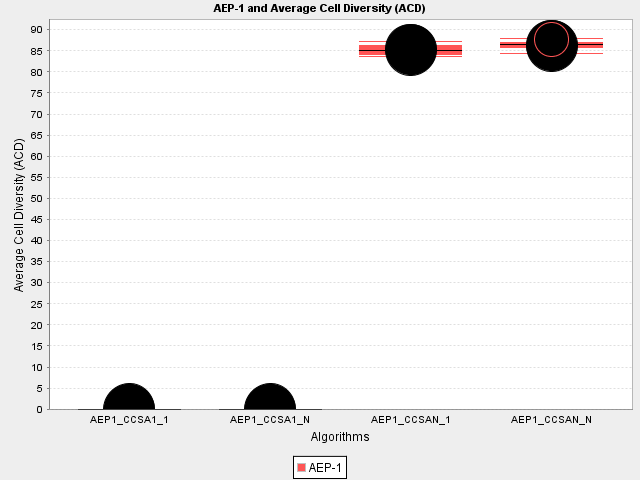
\includegraphics[scale=0.40]{Cells/CCSA-Study0-ACD}
	\end{minipage}}%
	%\hfill
	\subfloat[Average Cell Error (ACE) on ACSP-1.]{
	\label{fig:tissues:ccsa::study0:ace:boxplot} %% label 
	\begin{minipage}[t]{0.50\textwidth}
		\centering 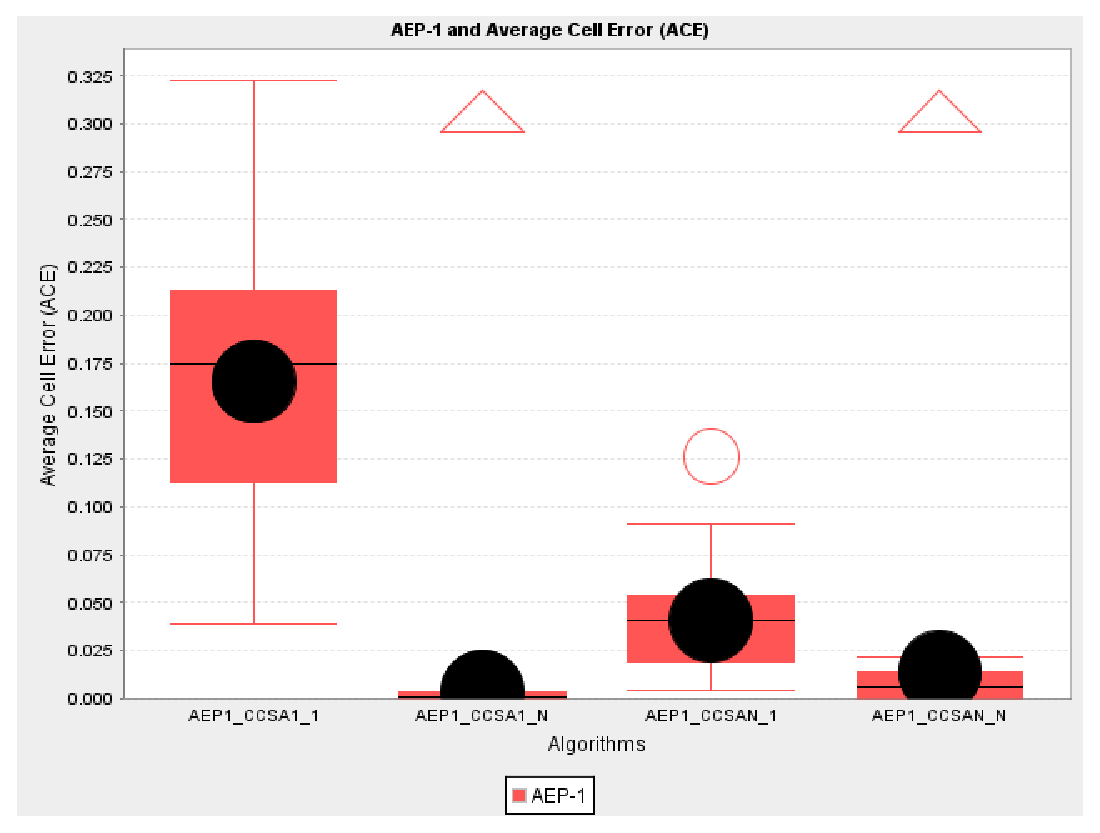
\includegraphics[scale=0.40]{Cells/CCSA-Study0-ACE}
	\end{minipage}}\\
	% new line for second set
	\subfloat[Average Cell Diversity (ACD) on ACSP-10.]{
	\label{fig:tissues:ccsa::study1:acd:boxplot} %% label 
	\begin{minipage}[t]{0.50\textwidth}
		\centering 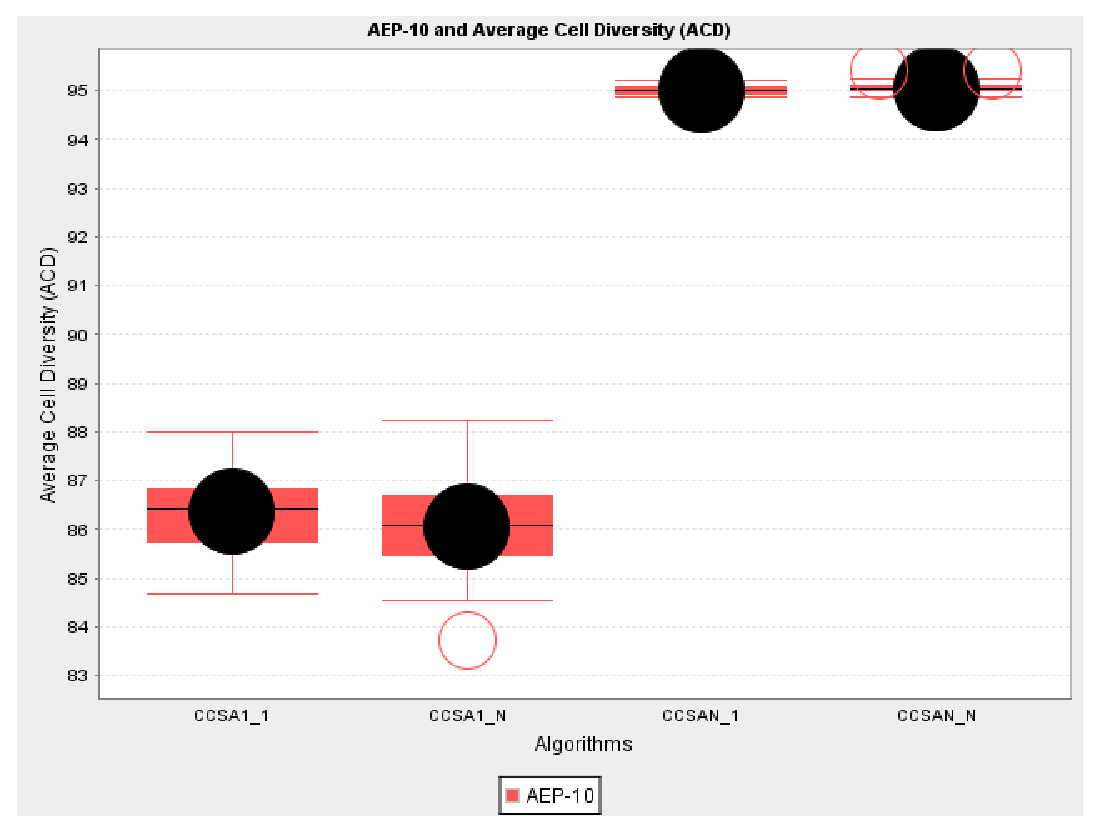
\includegraphics[scale=0.40]{Cells/CCSA-ACD}
	\end{minipage}}%
	%\hfill
	\subfloat[Average Cell Error (ACE) on ACSP-10.]{
	\label{fig:tissues:ccsa::study1:ace:boxplot} %% label 
	\begin{minipage}[t]{0.50\textwidth}
		\centering 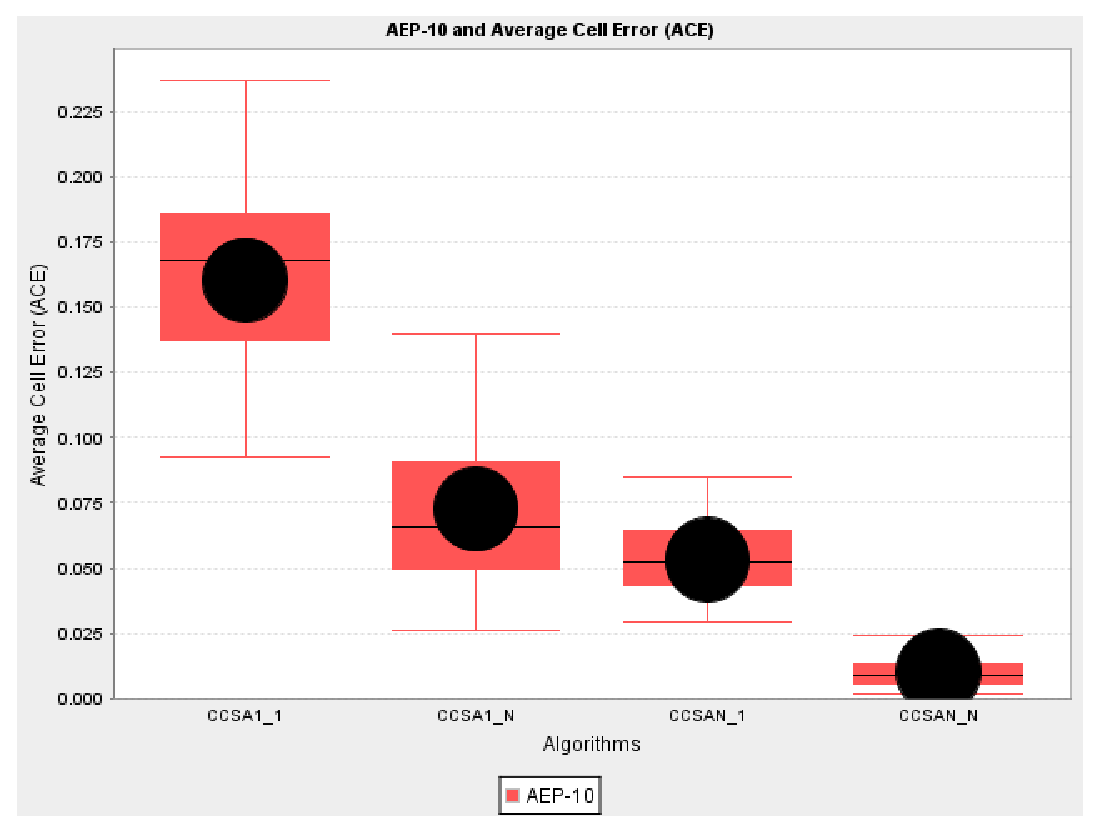
\includegraphics[scale=0.40]{Cells/CCSA-ACE}
	\end{minipage}}%
	\caption{Box-and-whisker plot's from the Cellular Empirical Study.}
	\label{fig:tissues:ccsa::study1:all:boxplot} %% label for entire figure
\end{figure}


% plots
\begin{figure}[htp]
	\subfloat[CCSA(N+N) on ACSP-1.]{
	\label{fig:cells:ccsa:acsp1:a} %% label 
	\begin{minipage}[t]{0.50\textwidth}
		\centering 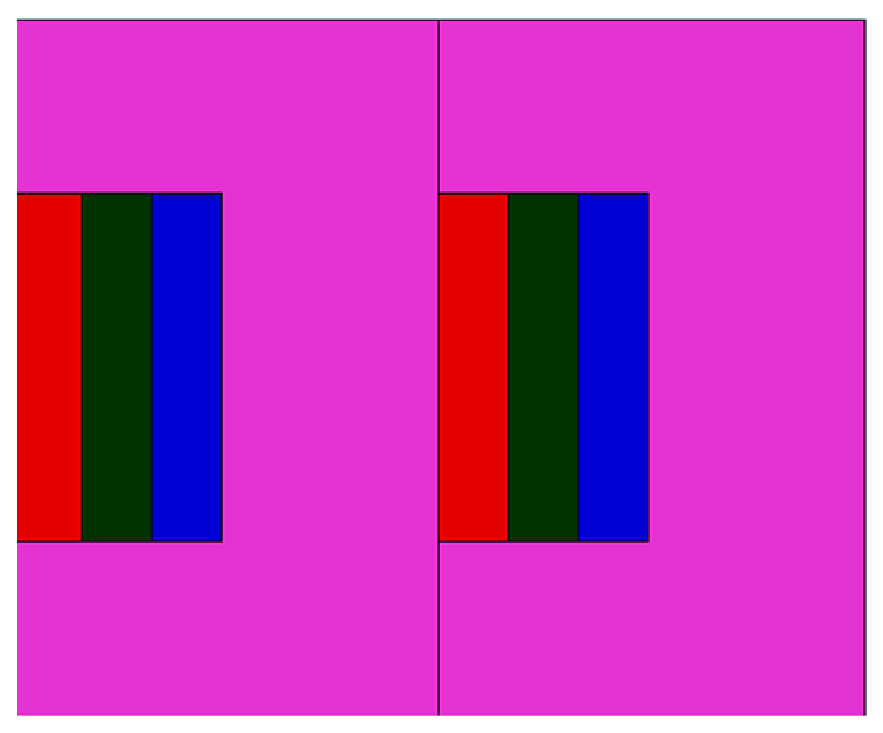
\includegraphics[scale=0.45]{Cells/CCSA(N+N)-ACSP-1}
	\end{minipage}}%
	\hfill
	\subfloat[CCSA(N+N) on ACSP-10.]{
	\label{fig:cells:ccsa:acsp10:b} %% label 
	\begin{minipage}[t]{0.50\textwidth}
		\centering 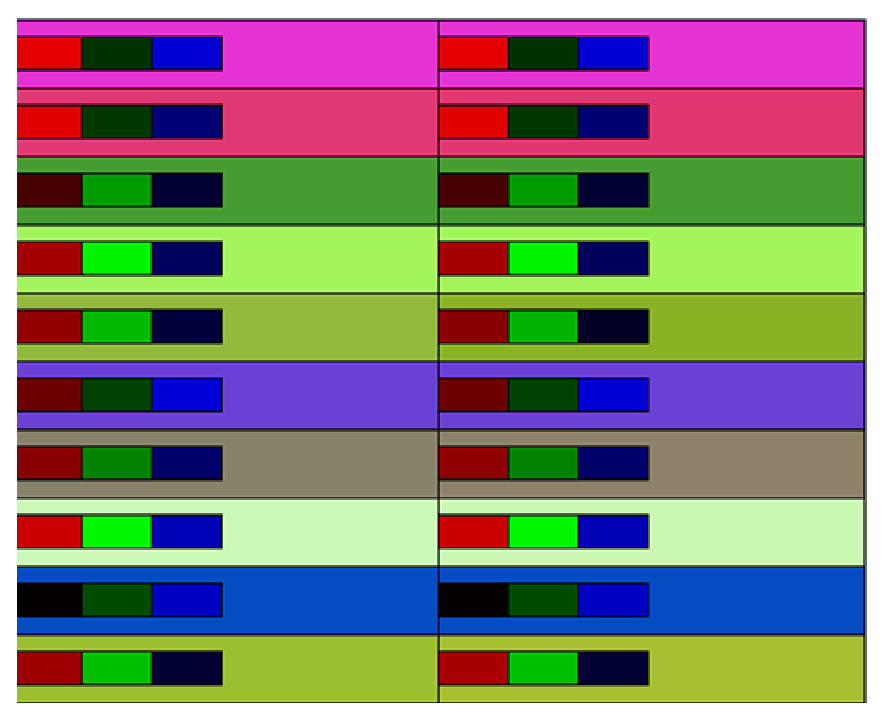
\includegraphics[scale=0.45]{Cells/CCSA(N+N)-ACSP-10}
	\end{minipage}}\\
	% end
	\caption{Example plots of $T_{rs}$ from the CCSA(N+N) at the end of the run on left section on both plots, for both ACSP-1 and ACSP-10, where the problem solution is represented on the right of each plot, and colour components within each CSP.}
	\label{fig:cells:ccsa:ccsa:plots} %% label for entire figure
\end{figure}


%
% Analysis
%
\subsubsection{Analysis}
This section provides an analysis of the results reported in the previous section in the context of the goals of the empirical study. Specifically, the analysis is broken down into the selection and clonal set size trends for small and large antigenic environments.

%
% Selection and Clonal Trends (ACSP-1)
% 
\paragraph{Selection and Clonal Trends (ACSP-1)}
% section
This section considers the selection and clonal trends of the CCSA configurations on ACSP-1.
% selection
The increase in the number of selected cells from 1 to $N$ resulted in a large increase in diversity as expected given the required shift in increase in the number of cells in the repertoire to support the increased selection size. The increase in the number of cells selected resulted in a decrease in error with a single clone and an increase when multiple clones were created.
% clone
The increase in the number of clones created for selected cells from 1 to $N$ resulted in very minor differences in the repertoire diversity, although did result in a large decrease in the average cell error.
% trends
The results confirmed the expectation that in the optimisation of a repertoire for a single antigen, the creation of more clones results in an improved system capability given that each clone represents a new trial and potential improvement over an already relatively good structure. 

%
% Selection and Clonal Trends (ACSP-10)
% 
\paragraph{Selection and Clonal Trends (ACSP-10)}
% section
This section considers the selection and clonal trends of the CCSA configurations on ACSP-10. 
% selection
The increase in the number of selected cells resulted in a decrease in the system error with a small repertoire, although in this case the trend held for both small and large repertoire sizes. 
% clone
The increase in the number of clones resulted in only very minor changes to the average cell diversity, although resulted in a consistent decrease in the the average cell error.
% trends
The increase in the size of the antigenic environment did not disrupt the general trend of increase number of clones resulting in increase system capability. Unlike the single antigen case, the increase in the number of selected cells also consistently resulted in a decrease in average cell error. 

%
% Conclusions
%
\subsubsection{Conclusions}
This section summarises the findings of the empirical study into the Cellular Clonal Selection Algorithm in terms of the primitives that were the focus of the study and the expectations that motivated the study.

\begin{enumerate}
		\item The Cellular Clonal Selection Algorithm successfully addressed 1 and 10 antigen problems, demonstrating itself as a viable realisation of a foundational clonal selection adaptive strategy under the circumstances considered.
		\item The increase in the number of selected cells (allocated resources) results in improved system capability with small cloning on the single antigen problem, although is consistently beneficial on the larger antigenic problem.
		\item The increase in the number of clones (trials) results in an improved system capability across the tested antigenic environments.	
\end{enumerate}


%
% Replacement Clonal Selection Empirical Study
%
\subsection{Replacement Empirical Study}
\label{sec:cells:ccsa:rcsa}

%
% Aim
%
\subsubsection{Aim}
The aim of this empirical study was to investigate the properties of the CCSA and the RCCSA as a viable realisation of cellular clonal selection that promote improved utilisation of repertoire resources. Improved utilisation will effect the composition and may effect the capabilities of a repertoire, where the promotion and maintenance of redundant perspectives is expected to provide benefits in terms of fault tolerance. Toward this end, the study had the following goals:

\begin{enumerate}
	\item Assess varied clonal integration mechanisms with CCSA that promote concurrent redundant perspectives of each antigen.
	\item Assess varied clonal integration mechanisms with RCCSA that promote concurrent perspectives and compare to CCSA.
\end{enumerate}

%
% Method
%
\subsubsection{Method}

%
% Problems
%
\paragraph{Problems}
This study used the ACSP-10 problem used for the CCSA empirical study in Section~\ref{sec:cells:ccsa:ccsa}.

% 
% Algorithms
%
\paragraph{Algorithms}
This section considers varied configurations of the CCSA and the RCCSA. The configuration parameters of each algorithm type are presented in Table~\ref{tab:cells:clonalselection:rccsa}. The chosen configurations of the repertoire, number of selected cells and number of clones facilitate the allocation of a maximum of six repertoire position per antigen.
% CCSA
The CCSA configurations included the CCSA(N+N) from CCSA empirical study in Section~\ref{sec:cells:ccsa:ccsa} as well as two extensions. CCSA(N+N)-G aggregates all clones into a single group which collectively compete with the $N_{selected}$ selected cells from the repertoire for their position. CCSA(N+N)-GS also aggregates all clones into a single clonal group, each of which competes with the same number of the best matching cells as there are in the clonal set drawn from the repertoire.
% RCSA
Two variations of the RCCSA algorithm (defined in Algorithm~\ref{alg:cells:realisation:algorithms:rccsa:exposure}) were assessed, both of which used Hamming Distance (Equation~\ref{eq:cells:realisation:hamming}) between cells in the replacement mechanism. The RCCSA-H configuration allowed clones to select the most similar cells in the repertoire to compete with for a position, whereas the RCCSA-H-ES configuration restricted selection to those cells in the repertoire that were not clonal siblings (hamming similarity excluding siblings). 

\begin{table}[htp]
	\centering\small
		\begin{tabular}{lllllll}
		\toprule
		\emph{CSA} & $N_{cells}$ & $N_{selected}$ & $N_{clones}$ & \emph{Clones ($A$)} & \emph{Positions} & \emph{Clones ($I$)} \\ 
		\toprule
		\emph{N+N} & 60 & 2 & 3 & 6 & 2 & 60 \\ 
		\emph{N+N-G} & 60 & 2 & 3 & 6 & 2 & 60 \\ 
		\emph{N+N-GS} & 60 & 2 & 3 & 6 & 6 & 60 \\ 
		\emph{RCCSA-H} & 60 & 2 & 3 & 6 & 6 & 60 \\ 
		\emph{RCCSA-H-ES} & 60 & 2 & 3 & 6 & 6 & 60 \\ 
		\bottomrule
		\end{tabular}
	\caption{Summary of the assessed configuration for the CCSA-RCCSA empirical study.}
	\label{tab:cells:clonalselection:rccsa}
\end{table}


%
% Experiment
%
\paragraph{Experiment}
This study used the same experimental configuration including stop conditions, measures, as were used for the CCSA empirical study in Section~\ref{sec:cells:ccsa:ccsa}. 
% ABMCPA
An additional measure was used to provide an assessment of the number of cells ($C$) in the repertoire ($T$) specialised to each antigen ($A$) in the scope of the problem ($I$). This measure is called the \emph{Average Best Matching Cells Per Antigen (ABMCPA)} defined in Equation~\ref{eq:cells:ccsa:rcca:abmcpa} that assessed and located the set of best matching cells for each antigen (Algorithm~\ref{alg:cells:ccsa:rccsa:bmc}) and averaged the number of cells returned for each antigen.

\begin{algorithm}[htp]
  \SetLine
  
  \SetKwData{Tissue}{T}
  \SetKwData{Antigen}{A}
  \SetKwFunction{Exposure}{Exposure}
  
  \KwIn{\Tissue, \Antigen}		
  \KwOut{$T_{BMC}$}
  
	$T_{BMC} \leftarrow$0\;
	\For{$C_i \in$ \Tissue}
	{
		\Exposure{\Antigen, $C_i$}\;
		% check for new set
		\uIf{${T_{BMC}}_n > 0$}
		{
			$C\prime \leftarrow {T_{BMC}}_i$\;
			\uIf{$C_i$.affinity $<$ $C\prime$.affinity}
			{
				% clear
				$T_{BMC} \leftarrow$0\;
				$T_{BMC} \leftarrow C_i$\;
			}
			\ElseIf{$C_i$.affinity $\equiv$ $C\prime$.affinity}
			{
				$T_{BMC} \leftarrow C_i$\;
			}
		}
		\Else
		{
			$T_{BMC} \leftarrow C_i$\;
		}		
	}
	\Return{$T_{BMC}$}\;
	
	\caption{Best Matching Cells (BMC's) for a given Antigen.}
	\label{alg:cells:ccsa:rccsa:bmc}	
\end{algorithm}



\begin{equation}
	AverageBMCPerAntigen(I,T) = \frac{1}{I_n} \sum_{i=1}^{I_n} {ABMCS(A_i, T)}_n
	\label{eq:cells:ccsa:rcca:abmcpa}
\end{equation}


%
% Results
%
\subsubsection{Results}
% tables
Table~\ref{tab:cells:ccsa:rccsa} provides a summary of results for each algorithm-problem combination including the mean ($\bar{x}$) and standard deviation ($\sigma$) of collected measure values. The non-parametric Mann-Whitney~U statistical test was calculated pair-wise for all algorithms. 
% figures
Figures \ref{fig:tissues:ccsa:rccsa:acd:boxplot}, \ref{fig:tissues:ccsa:rccsa:ace:boxplot}, and \ref{fig:tissues:ccsa:rccsa:abmca:boxplot} show the ACD, ACE, and ABMCPA on all algorithms respectively. 
% plots
Figure~\ref{fig:cells:ccsa:rccsa:plots} provides example plots of the state of the repertoire (left of each plot) compared to the problem domain (right of each plot) from each of the five algorithms (same configuration, random seeds of 1 and 5 for the algorithm and problem respectively). 

\begin{table}[htp]
	\centering\small
		\begin{minipage}{0.80\textwidth}		
		  \centering
			\begin{tabular}{llllllll}			
			\toprule
			\textbf{Problem} & \textbf{System} & \multicolumn{2}{c}{\textbf{ACD}} & \multicolumn{2}{c}{\textbf{ACE}} & \multicolumn{2}{c}{\textbf{ABMCPA}}\\
			\midrule
			\emph{ACSP} & \emph{CSA} & $\bar{x}$ & $\sigma$ & $\bar{x}$ & $\sigma$ & $\bar{x}$ & $\sigma$\\
			\toprule
			ACSP-10 & CCSA(N+N) & 94.356 & 0.171 & 0.027 & 0.012 & 1 & 0 \\
			ACSP-10 & CCSA(N+N)-G & 93.995 & 0.24 & 0.023 & 0.014 & 1.82 & 0.124 \\
			ACSP-10 & CCSA(N+N)-GS & 88.456 & 0.937 & 0.062 & 0.015 & 4.907 & 0.528 \\
			ACSP-10 & RCCSA-H & 94.37 & 0.18 & 0.03 & 0.013 & 1 & 0 \\
			ACSP-10 & RCCSA-H-ES & 88.083 & 0.79 & 0.028 & 0.013 & 2.653 & 0.385 \\
			\multicolumn{2}{l}{\emph{Significant}} & True\footnote{False for CCSA(N+N) and RCCSA-H} &  & True &  & True\footnote{False for CCSA(N+N) and RCCSA-H} & \\
			\bottomrule
			\end{tabular}			
		\end{minipage}
	\caption{Summary of results from the CCSA-RCCSA empirical study on ACSP-10.}
	\label{tab:cells:ccsa:rccsa}
\end{table}

\begin{figure}[htp]
	\subfloat[Average Cell Diversity (ACD) on ACSP-10.]{
	\label{fig:tissues:ccsa:rccsa:acd:boxplot} %% label 
	\begin{minipage}[t]{0.50\textwidth}
		\centering 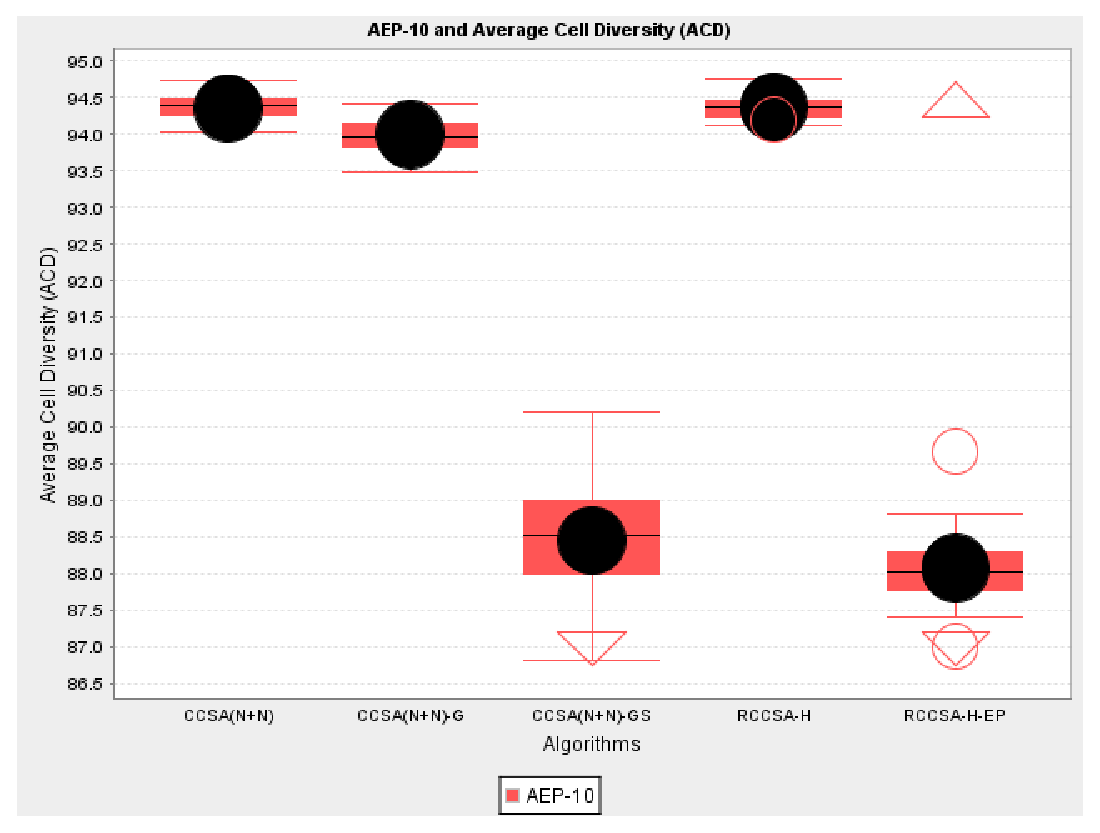
\includegraphics[scale=0.40]{Cells/CCSA-Study2-ACD}
	\end{minipage}}%
	\hfill
	\subfloat[Average Cell Error (ACE) on ACSP-10.]{
	\label{fig:tissues:ccsa:rccsa:ace:boxplot} %% label 
	\begin{minipage}[t]{0.50\textwidth}
		\centering 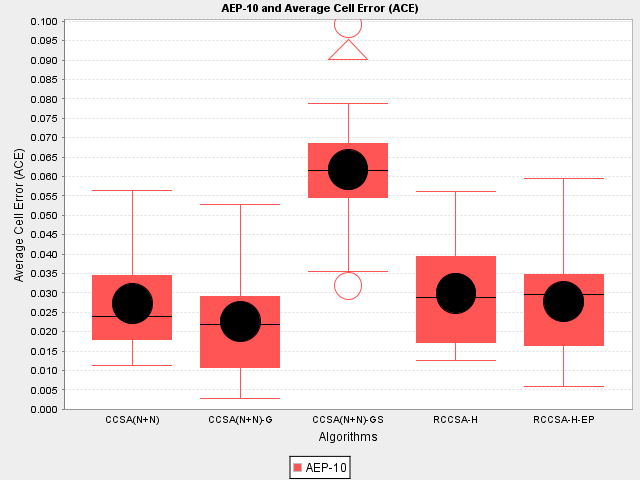
\includegraphics[scale=0.40]{Cells/CCSA-Study2-ACE}
	\end{minipage}}\\
	%\hfill
	\subfloat[Average BMC Per Antigen (ABMCPA) on ACSP-10.]{
	\label{fig:tissues:ccsa:rccsa:abmca:boxplot} %% label 
	\begin{minipage}[t]{\textwidth}
		\centering 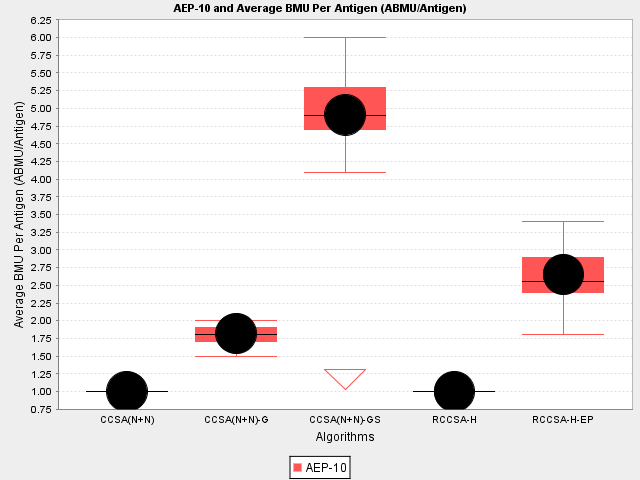
\includegraphics[scale=0.40]{Cells/CCSA-Study2-ABMCA}
	\end{minipage}}%
	\caption{Box-and-whisker plot's from the Replacement Empirical Study.}
	\label{fig:tissues:rccsa::study2:all:boxplot} %% label for entire figure
\end{figure}

% plots
\begin{figure}[htp]
	\subfloat[CCSA(N+N).]{
	\label{fig:cells:ccsa:rccsa:a} %% label 
	\begin{minipage}[t]{0.50\textwidth}
		\centering 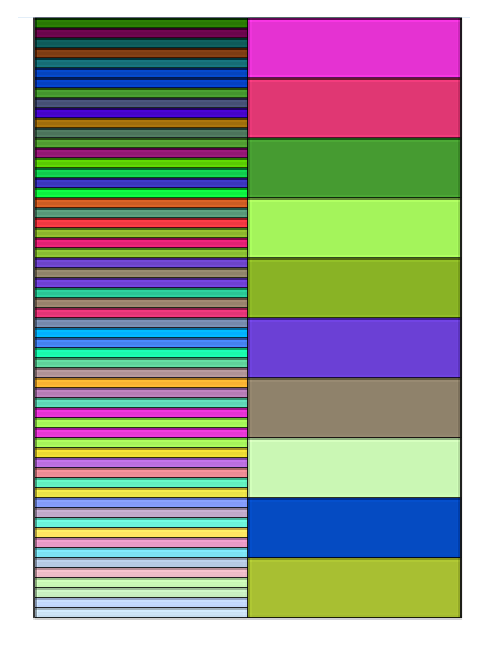
\includegraphics[scale=0.45]{Cells/CCSA(N+N)-plot}
	\end{minipage}}%
	\hfill
	\subfloat[(N+N)-G.]{
	\label{fig:cells:ccsa:rccsa:b} %% label 
	\begin{minipage}[t]{0.50\textwidth}
		\centering 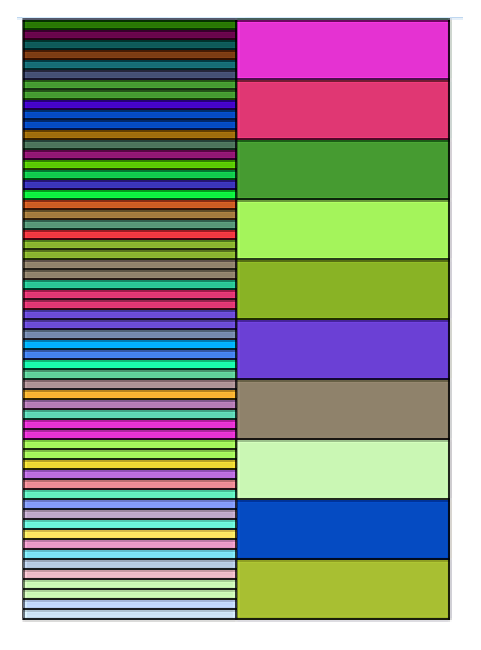
\includegraphics[scale=0.45]{Cells/CCSA(N+N)-G-plot}
	\end{minipage}}\\
	% new line for second set	
	\subfloat[(N+N)-GS.]{
	\label{fig:cells:ccsa:rccsa:c} %% label 
	\begin{minipage}[t]{0.50\textwidth}
		\centering 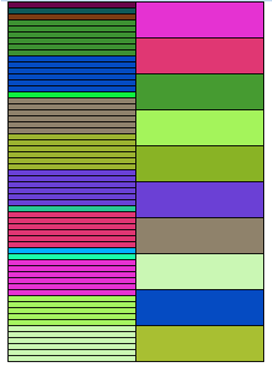
\includegraphics[scale=0.45]{Cells/CCSA(N+N)-GS-plot}
	\end{minipage}}%
	\hfill
	\subfloat[RCCSA-H.]{
	\label{fig:cells:ccsa:rccsa:d} %% label 
	\begin{minipage}[t]{0.50\textwidth}
		\centering 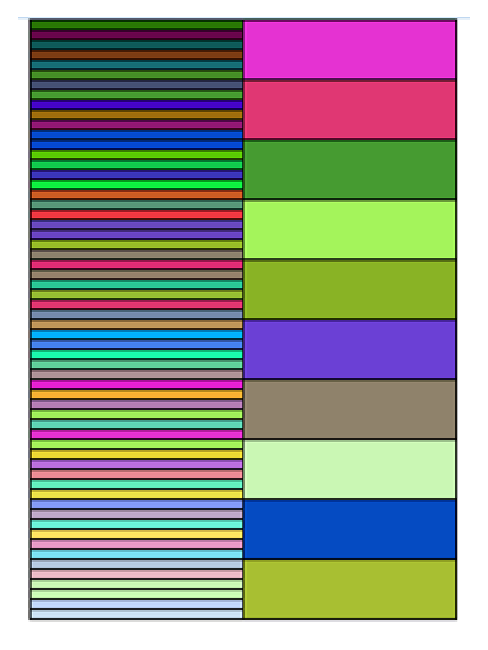
\includegraphics[scale=0.45]{Cells/RCCSA-H-plot}
	\end{minipage}}\\
	% new line for third set	
	\subfloat[RCCSA-H-ES.]{
	\label{fig:cells:ccsa:rccsa:e} %% label 
	\begin{minipage}[t]{\textwidth}
		\centering 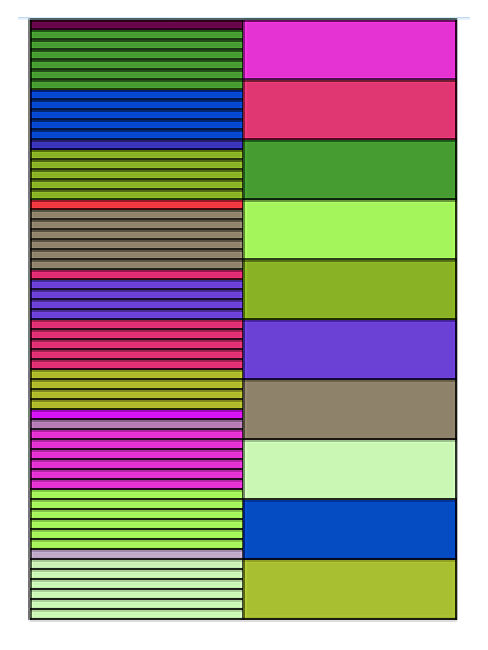
\includegraphics[scale=0.45]{Cells/RCCSA-H-ES-plot}
	\end{minipage}}	
	% end
	\caption{Plots of the ordered state of the repertoire after the triggering of the stop condition (left of each plot) for the assessed CCSA and RCCSA algorithms on the ACSP-10, where the right of each plot provides the problem optima.}
	\label{fig:cells:ccsa:rccsa:plots} %% label for entire figure
\end{figure}


%
% Analysis
%
\subsubsection{Analysis}
This section provides an analysis of the results reported in the previous section in the context of the goals of the empirical study. 

%
% CCSA Trends
%
\paragraph{CCSA Trends}
% section
% This section considers the behaviour trends of the CCSA and varied replacement mechanisms. 
% diversity
With regard to average cell diversity, the aggregation and thus competition between the entire clonal set with the selected set resulted in a slight drop in diversity, although the relaxing of the competition from progenitor cells to the entire repertoire resulted in a further larger decrease in diversity by $\approx 5.5$ bits.
% error
Interestingly the CCSA(N+N)-G achieved a slightly lower error than CCSA(N+N) where the further relaxation of competition in CCSA(N+N)-GS resulted in a large relative increase in the ACE.
% bmu 
Correlating with the decrease in ACD, the relaxation in the integration of the clones resulted in an increase in the number of best matching cells (BMC's) per antigen, rising to an average of $\approx 5$ in the case of CCSA(N+N)-GS.
% trends
The results demonstrate that multiple concurrent and redundant perspectives of antigen can be achieved by relaxing the replacement competition in CCSA which decreases repertoire diversity. The results also highlight that competition between the clonal set results in an improved result in terms of ACE and ABMCPA over CCSA(N+N), although the relaxation from progenitor set to whole repertoire dramatically increases ABMCPA at expense of increasing the systems general capability. The specialisation of each antigen's cellular imprint in the repertoire provided by CCSA(N+N)-GS is clearly demonstrated in Figure~\ref{fig:cells:ccsa:rccsa:c} compared to CCSA(N+N)-G in Figure~\ref{fig:cells:ccsa:rccsa:b}.

%
% RCCSA Trends
%
\paragraph{RCCSA Trends}
% section
% This section considers the behaviour trends of the RCCSA and the two replacement mechanisms. 
% diversity
The exclusion of clonal siblings from replacement resulted in a significant decrease in diversity, the same seen between CCSA(N+N)-G and CCSA(N+N)-GS. 
% error
The exclusion of progeny also resulted in a very slight decrease in ACE over RCCSA-H.
% bmu
Interestingly, the repertoire-wide competition between the aggregated clonal set in RCCSA-H resulted in a single average BMC per antigen, whereas, the exclusion of progeny during replacement promoted the competition between the concurrent clonal set such that ABMCPA increased to $\approx 2.5$.
% trends
Also interesting was that the ACE and ABMCPA results for RCCSA-H were not significantly different from CCSA(N+N), demonstrating that unrestricted similarity-affinity based replacement into the repertoire behaves much like CCSA(N+N) confirming the expectation that motivated the exclusion of clonal progeny: that they are more similar. Also interesting is that the increase in ABMCPA with RCCSA-H-ES also resulted in a relative increase in ACE compared to CCSA(N+N) and CCSA(N+N)-G, suggesting that for the mechanisms used, increasing the specialisation of the cellular footprint for each antigen comes at the expense of general repertoire competence. 

%
% Conclusions
%
\subsubsection{Conclusions}
This section summarises the findings of the empirical study into the CCSA and RCCSA in terms of the primitives that were the focus of the study and the expectations regarding proportional resource allocation.

\begin{enumerate}
		\item Relaxing the constraints for competition in the integration clones into the repertoire results in increased number of concurrent redundant perspectives of an antigen in the repertoire for CCSA and RCCSA.
		\item Strong inter-clonal competition in CCSA results in improved performance with a slight increase in size in the number of redundant perspectives.
		\item Repertoire-wide integration restrained by only similarity-and-affinity in RCCSA approximates CCSA(N+N) in behaviour.
		\item Repertoire-wide integration restrained by affinity in CCSA or by similarity-and-affinity-exclusion in RCCSA results in a large increase in the size and quality of the number of redundant perspectives at the cost of general repertoire capability under both algorithms. 		
\end{enumerate}

%
% Degenerate Clonal Selection Empirical Study
%
\subsection{Degenerate Empirical Study}
\label{sec:cells:ccsa:dcsa}
There is a lack of a one-to-one correspondence between antigen and receptors in the acquired immune system. A given antigen may have the capacity to trigger a very larger number of receptors, therefore resulting in a polyclonal activation, although a response is typically oligoclonal. This may be accounted for by the competition between clones for selection by the antigen. In addition, a given receptor may respond to a large number of antigens, thus resulting in a polyclonal response, something that cannot be accounted for by the clonal selection theory. In the Cognitive Theory of Immunology, Cohen refer to this polyclonal response of a given receptor as \emph{cellular degeneracy}, where those receptors that are without a context are cross-specific, including auto-specific \cite{Cohen2004}. A polyclonal response is the antithesis of clonal dominance (a feature that underlies the clonal selection theory). The solution as proposed in cognitive theory is that specificity is an emergent phenomenon \cite{Cohen2001, Hershberg2003}. Unlike the clonal selection theory, where specificity is a property of antigen-receptor interaction, emergent specificity is a down-stream effect that occurs after the initial interaction. A collection of varied and communicating cell types respond to the antigen in context. This is the so-called meta-response of cognitive theory, called the co-response or corespondence. The degeneracy of cell signalling is proposed as the basis of plasticity both in the brain and in the immune system, and is the feature exploited by antibiotics and pharmaceuticals.

\begin{figure}[htp]
	\centering
	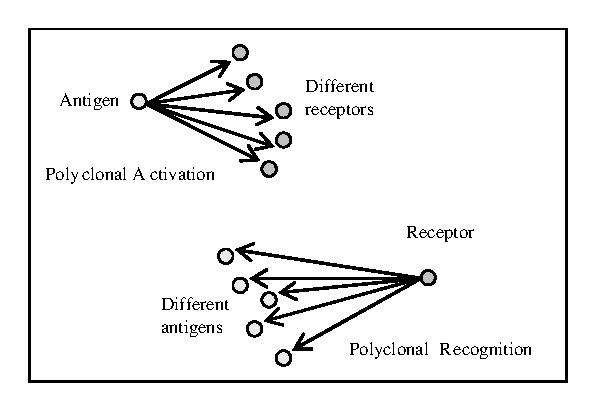
\includegraphics[scale=0.85]{ClonalSelection/cognitive-polyclonal}
	\caption{Depiction of a polyclonal activation and a polyclonal response.}
	\label{pic:cognitive:polyclonal}
\end{figure}

% general properties i care about
Clonal selection accounts for the restriction of a potential polyclonal activation of the repertoire to an oligoclonal activation by dominant clones out competing the less well fitted clones (referred to as clonal dominance). The classical theory does not account for lack of one-to-one correspondence between cells and antigen (the cross-reactivity of receptors referred to as polyclonal response). Cognitive immune theory accounts for polyclonal response between antigen and receptors by suggesting (1) that cells in isolation are degenerate and cross-specific, (2) context defines the use for degenerate cells resulting in emergent specificity.

%
% Aim
%
\subsubsection{Aim}
Section~\ref{sec:cells:realised:trends} considered the expectations of clonal selection on a degenerate repertoire, specifically with regard to the pressures required to facilitate polyclonal activation and response. The aim of this empirical study is to investigate these expectations in the context of cellular clonal selection. 
% goals
Toward this end, the study had the following goals:

\begin{enumerate}	
	\item Investigate a clonal selection with a degenerate representation.
	\item Assess selective pressures and explicit aggregation to constrain polyclonal activation and response.	
\end{enumerate}

%
% Method
%
\subsubsection{Method}

%
% Problems
%
\paragraph{Problems}
% analogy
The definition of the Colour Space Domain in Section~\ref{subsec:cells:paradigm:colourspace} highlighted a `retina and colour perception' analogy made by Cohen to describe cellular degeneracy and emergent specificity. The problems in this section are motived by that analogy.
% same things
This study used the ACSP-10 problem used for the CCSA empirical study in Section~\ref{sec:cells:ccsa:ccsa}, although evaluated on a per colour component basis. To differentiate this mode of evaluation from the holistic ACSP, it is referred to as the Determinant Colour Space Problem (DCSP-10).
% Components
A degenerate colour representation was used called component degeneracy where each colour was divided into the its Red, Green, and Blue components. Components are denoted $D$, where a $A = \{D_1, D_2, D_3\}$ for each colour space pattern. Degenerate component cells were assessed using Equation~\ref{eq:cells:realised:component:distance}, where each degenerate component cell was defined by a 64-bit bitstring and decoded to a real value using Gray Code (Equation~\ref{eq:cells:realised:graycode}). Components were considered a symbolic degenerate representation as each component has direct meaning via their linear aggregation in the the context of a colour space pattern.

% Component Distance
\begin{equation}
	ComponentDistance(D, C) = \left| D - C \right|
	\label{eq:cells:realised:component:distance}
\end{equation}

% 
% Algorithms
%
\paragraph{Algorithms}
The study considers a \emph{Degenerate Cellular Clonal Selection Algorithm (DCCSA)} as an extension of the RCCSA (defined in Algorithm~\ref{alg:cells:realisation:algorithms:rccsa:exposure}) that uses a degenerate representation. RCCSA was selected as a base algorithm because (1) it achieves adequate results in terms of repertoire capability, and (2) because it achieves multiple high-affinity concurrent perspectives (proportional repertoire composition) on antigen to which it is exposed.
% component
The RCCSA was configured with the following configuration: $N_{cells}=100$, with $N_{selected}=3$, and $N_{clones}=1$ per determinant exposure, resulting in a resource allocation of three cells per component, or nine cells per antigen. A Hamming-based similarity assessment was used in replacement, with clonal sibling exclusion. Two variations of the degenerate cellular component selection were considered as follows: (1) explicit per-component selection called DCCSA-E, and (2) pre-committed component cells called DCCSA-P. Both approaches aggregated the best degenerate cell for each component into a holistic solution to address each given antigen in the ACSP. Explicit per-component selection maintained a repertoire of uncommitted components that were assessed and selected in the context of each component of each colour space pattern. This allowed degenerate cell reuse across the components of a single antigen and across the components of multiple antigen. Pre-committed component cells involved the management of one sub-repertoire for each component, where the size of each repertoire was a fraction of the total number of cells ($\lfloor \frac{1}{N_{components}} \times N_{cells}\rfloor$). 


%
% Experiment
%
\paragraph{Experiment}
% same things
This study used the same experimental configuration including stop conditions, measures, as were used for the CCSA empirical study in Section~\ref{sec:cells:ccsa:ccsa}. 
% component
An additional measure was introduced for the degenerate component algorithms that assessed the extent of the cross-reactivity of the repertoire called the \emph{Average Polyclonal Response Error (APRE)}, defined in Equation~\ref{eq:cells:ccsa:dccsa:apre}. APRE provides an indication of the average repertoire error per component. 
% APRE
\begin{equation}
	% across all antigen
	APRE(I, T) = \frac{1}{I_n \times {A_i}_n} \sum_{i=1}^{I_n}
	% across all components
	\left(\sum_{j=1}^{{A_i}_n}
	% across the entire repertoire
	\left(\frac{1}{T_n} \sum_{k=1}^{T_n}
	% component distance
	ComponentDistance({A_i}_j, C_k)	
	\right)\right)
	\label{eq:cells:ccsa:dccsa:apre}
\end{equation}


%
% Results
%
\subsubsection{Results}
% tables
Table~\ref{tab:cells:ccsa:dccsa} provides a summary of results for each algorithm-problem combination including the mean ($\bar{x}$) and standard deviation ($\sigma$) of collected measure values. The non-parametric Mann-Whitney~U statistical test was calculated pair-wise for all algorithms. 
% figures
%Figure~\ref{fig:tissues:ccsa:dcccsa:ace:boxplot} shows the ACS on both algorithms. 

\begin{table}[htp]
	\centering\small
		\begin{tabular}{llllllll}
		\toprule
		\textbf{Problem} & \textbf{System} & \multicolumn{2}{c}{\textbf{ACD}} & \multicolumn{2}{c}{\textbf{ACE}} & \multicolumn{2}{c}{\textbf{APRE}}\\
		\midrule
		\emph{AEP} & \emph{CSA} & $\bar{x}$ & $\sigma$ & $\bar{x}$ & $\sigma$ & $\bar{x}$ & $\sigma$\\
		\toprule
		DCSP-10 & DCCSA-E & 31.638 & 0.047 & 0.003 & 0.001 & 0.333 & 0.018 \\
		DCSP-10 & DCCSA-P & 31.627 & 0.059 & 0.008 & 0.003 & 0.334 & 0.019 \\
		\multicolumn{2}{l}{\emph{Significant}} & False &  & True &  & False & \\
		\bottomrule
		\end{tabular}
	\caption{Summary of results from the DCCSA empirical study on DCSP-10.}
	\label{tab:cells:ccsa:dccsa}
\end{table}

%\begin{figure}[htp]
%	\centering
%		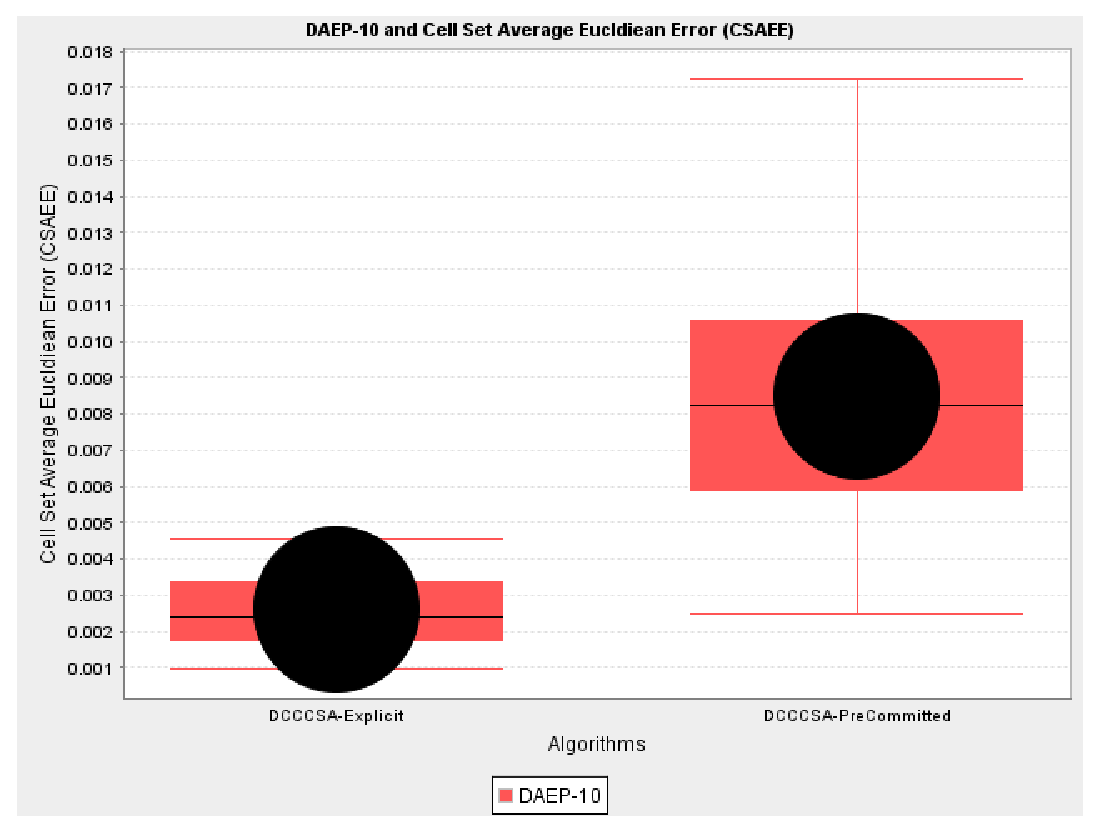
\includegraphics[scale=0.35]{Cells/DCCCSA-ACE}
%	\caption{Box-and-whisker plot of Average Cell Error (ACE) on DCSP-10.}
%	\label{fig:tissues:ccsa:dcccsa:ace:boxplot}
%\end{figure}

%
% Analysis
%
\subsubsection{Analysis}
This section provides an analysis of the results reported in the previous section in the context of the goals of the empirical study, specifically (1) restrictive selection, and (2) explicit aggregation. 

%
% Restrictive Selection
%
\paragraph{Restrictive Selection}
The results showed little significant difference on the selected measures between the explicit and pre-committed selection mechanisms, other than a slightly improved cell error for the explicit approach. The strong similarity in results, in particular the Average Polyclonal Response Error demonstrate that the degenerate component clonal selection was generally unaffected when the repertoire was split into sub-repertoires per component compared to an integrated cross-component competitive repertoire. The minimum Hamming distance between generated colour space patterns likely resulted in little cross-colour space pattern reuse given the per-pattern/per-component specialisation of the repertoire, and the lack of difference between segregated and integrated component repertoires.
% pervasive polyclonal activation
An important consideration is that CCSA and RCCAS implicitly rely on restrictive selection to bound polyclonal activation of cells. This is clear if we consider a principle of cellular clonal selection that the scope of the repertoire available allowing $N_{cells}$ interactions (assessments and activations). Without constrained selection, the scope of repertoire would respond in its entirety each antigen exposure.

%
% Explicit Aggregation
%
\paragraph{Explicit Aggregation}
The clonal selection strategy by-design continues regardless of the integration of the product of exposure events. With respect to the problem domain, aggregation of the product of exposures is the critical concern of a degenerate representation. The chosen degenerate component representation was chosen because of its easy linear aggregation of the best matching components, always resulting in feasible aggregated responses at the per-$D$, per-$A$, and per-$I$ levels.
% sub-symbolic
One may consider a sub-symbolic representation for the ACSP that does not easily aggregate into holistic colour space patterns solutions, such as sub-bitstrings. This is an important example because it highlights that such representation does not hinder the clonal selection strategy. Degenerate sub-strings may be assessed based on hamming distances from exposed $A$'s or $D$'s providing enough information for selection, cloning and integration. The explicit aggregation of sub-strings is less natural than the component case, requiring perhaps a per-bit position frequency assessment and a deterministic or probabilist generation of a viable holistic solution at the $A$ scale. The example highlights that explicit aggregation may be suitable for the linear aggregation of components, although becomes more difficult with sub-symbolic representations one which clonal selection can still operate effectively. 
% pervasive degeneracy
Explicit aggregation also highlights that this problem-centric concern is scale independent, where the components of a colour, and the colours of a colour set are the linear aggregation of selected information which may or may not be the case for more elaborate applications.

%
% Conclusions
%
\subsubsection{Conclusions}
This section summarises the findings of the empirical study into the DCCSA in terms of the primitives that were the focus of the study and the expectations regarding proportional resource allocation.

\begin{enumerate}
	% primitives
	\item \emph{Degenerate Components}
	\begin{enumerate}
		\item Clonal Selection on components provides a viable realisation of cellular degeneracy under the circumstances considered where strong selection and aggregation can constrain polyclonal activation.
		\item A RCCSA results in little difference in the partitioning or aggregation of the repertoire and thus competition of degenerate cells, suggesting clonal independence promoted via replacement is sufficient for non-overlapping clonal specialisation (assuming a large enough repertoire).
		\item Explicit aggregation provides a context in which to bound polyclonal response to strongly activated (selected) structures.
	\end{enumerate}
	
	% findings
	\item \emph{Selection and Aggregation}
	\begin{enumerate}
		\item Strong selection is required in all cellular clonal selection algorithms to manage the implicit polyclonal activation that occurs as a result of each antigens interaction with the entire repertoire.
		\item Aggregation is independent of the principle clonal selection operations, requiring explicit integration into the process (for those applications that operate on sub-solution structures).
	\end{enumerate}
	
\end{enumerate}


%
% Spatial Repertoire
%
\section{Spatial Repertoire}
\label{sec:cells:spatial}
This section considers a spatial context as a method for forming relationships between units undergoing clonal selection and expansion. A spatial clonal selection paradigm is investigated which outlines a fixed lattice structured repertoire on which clonal selection operators are applied. 

%
% Spatial Clonal Selection
%
\subsection{Spatial Clonal Selection}
% metaphor
The processes of selection and maturation of lymphocytes occurs in the spatially distributed confines of the host organism lymphatic system \cite{Anderson1990a}. Further, the spatial organisation may be required to provide context to guide emergent specificity \cite{Cohen2001a}. 
% abstraction
The competition in the clonal selection principle is between cells for resources in the repertoire. Competition can be facilitated through differential selection of an activated set which results in differential allocation of resources for clones from the activated set. In envisaging the repertoire as a spatial structure, an additional level of competition is introduced called \emph{spatial competition}. This competition puts pressure on cells in the same spatial neighbourhood to compete with each other. This pressure may be used for either the activation of cells during \emph{selection} or \emph{replacement} by clones of activated cells. A simple one or two-dimensional lattice structure may be used in which receptors occupy grid positions of the lattice, and the ends of the structure wrap around (ring or toroid), removing edge effects. The structure may be an equally arbitrary number of dimensions, although low dimensionality facilitates visualisation. Such a spatial repertoire structure provides a manifestation of the space complexity limits imposed on repertoire size, and imposes relationships between arbitrary neighbouring receptors for a given antigenic stimulus. 

\begin{figure}[ht]
	\centering
	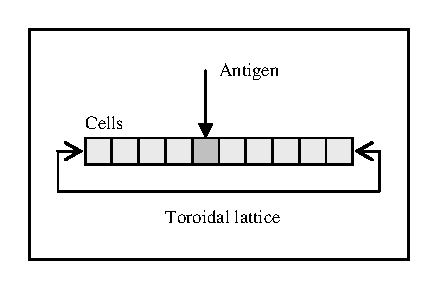
\includegraphics[scale=0.85]{Cells/cells-spatial-oned-lattice}
	\caption{Depiction of a one-dimensional toroidal lattice.}
	\label{pic:cells:spatial:lattice}
\end{figure}

%
% Spatial Selection
%
\subsubsection{Spatial Selection}
The spatial structure may be exploited in the selection of the activated set for a given antigen. In the selection scheme the repertoire is evaluated, scanned for the highest affinity cell, which is returned to address the needs of the antigen, and an activated set is selected from the high-affinity cells. Therefore, the conventional activated set may be conceptualised as the selection of cells from across the spatial structure. 
% usage
One may partition antigenic signals and match them to regions (logical partitions) of the spatial structure, such that regions are directed in a top-down manner to be responsible for specific antigenic signals. The input space can be partitioned by a measure relevant to the representation of the antigen or the cells in the repertoire. This partitioning scheme would be implemented such that activated sets of receptors may only be drawn from the allocated region of the spatial structure, therefore putting pressure on the region to produce and develop receptors suitable to the allocated portion of the input space. A concern with this approach is that information effective for representational partitions may be developed outside of allocated regions and thus would not be exploited (for example the cross-reactive response for generalisation). Further, without inter-region competition, the partitions may be considered isolated repertoires such that the partitioning prevents the take-over or resizing of spatial regions with proportion to signal frequency and complexity (an effect maintained by differential resource allocation across the whole repertoire). 

%
% Spatial Replacement
%
\subsubsection{Spatial Replacement}
The Replacement CCSA investigated in Section~\ref{sec:cells:ccsa:rcsa} may be elaborated to exploit a spatial structure such that replacement competition is \emph{spatially localised} or constrained to the locations in the repertoire that responded strongest to an antigenic stimulus. Competition for resources may be constrained to the spatially local neighbourhood of high affinity cells. The principle parts of a spatial replacement mechanism are as follows: a structured repertoire or \emph{lattice} data structure in which grid positions represent cells, a \emph{neighbourhood function} that identifies the scope of competition (see Figure~\ref{pic:cells:spatial:clones}), and a \emph{competition function} that defines how resources (lattice positions) are allocated to clones of selected cells.
% 2d
Spatial competition introduces spatial meaning between positions in the lattice, such that visualisation of the lattice can highlight relationships and facilitate the extraction of qualitative information from the repertoire. 

\begin{figure}[ht]
	\centering
	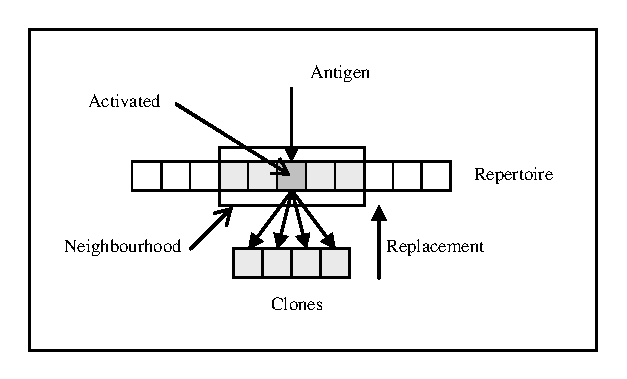
\includegraphics[scale=0.85]{Cells/cells-spatial-process}
	\caption{Depiction of clones competing in the neighbourhood of their progenitor.}
	\label{pic:cells:spatial:clones}
\end{figure}

% responsibility
The spatially restricted `back-end' selection (neighbourhood function) is expected to result in the assignment of antigenic-responsibility to regions of the spatial repertoire structure\footnote{`Back-end' refers to competition at the end of an iteration of the algorithm cycle.}. Therefore, the neighbourhood function constrain's resource allocation resulting in a localised clonal dominance effect, where those cells that win upfront selection will produce clones that dominate sub-structures in the lattice. In effect, the spatial replacement strategy facilitates a mapping of the antigenic space onto the lower-order topology of the spatial repertoire. The clonal selection axiom of `similar cells taking responsibility for similar antigen' is bonded to the lattice structure, facilitating the self-organisation of receptors to input signals. Ultimately, the expected organisation of similar cells into regions results in a broader competition between regions for activation, cloning, and the resulting ongoing retention of the region for spatial resources.
% replacement
The selection of the replacement function can play an important role in the maintenance behaviour of cell clusters. Clones are expected to have the same or similar affinity for the antigen as the activated cell given relatively low mutation rates. A clone that displaces a neighbouring cell is likely to be an activated cell in the following exposure. A similarity or affinity based replacement function is expected to maintain a cell cluster tied to a spatial locality and a random replacement function is expected to shift the centroid of the cluster around such that the fringe of the cell group may interact with neighbouring groups. In the case of the a stable spatial locality, upfront dominant cells are expected to put pressure on their neighbourhood to conform to the antigenic signals to which they dominant. Dominance leads to neighbourhood takeover which results in the emergent effect of self-organised responsibility. 

%
% Explicit and Implicit Organisation
%
\subsubsection{Explicit and Implicit Organisation}
Exploitation of the spatial structure as an upfront pressure results in the partitioning of input signals to regions of the spatial structure. This has the benefit of explicitly limiting the scope of interest of input signals space for regions of the lattice, with the problems associated with making assumptions regarding the partitioning the signal space. All resources are employed for a specific task, although not all the allocated resources may be required for their allocations. The exploitation of the spatial structure as a back-end pressure results in the implicit partitioning of the input space and self-organisation of receptor clones to take responsibility for the automatic partitions. This has the benefit of proportionate allocation (specialisation) of resources for the automatically identified complexities of the input space with the computational and delay costs for the self-organising process. Resource allocation is determined automatically, although not all resources may be utilised effectively. An interesting observation is that one method will lead to the other, such that the explicit exploitation of the spatial competition of both ends is not required. The application of upfront spatial partitioning will force regions to adapt to input signals, thus result in replacements occurring in the same region, reinforcing the partitioning. The application of back-end partitioning will self-organise the responsibility for antigenic signals via replacement, which will reinforce future input signals being directed to responsible areas of the spatial structure.

\begin{figure}[ht]
	\centering
	\begin{minipage}[c]{0.5\linewidth}
		\centering 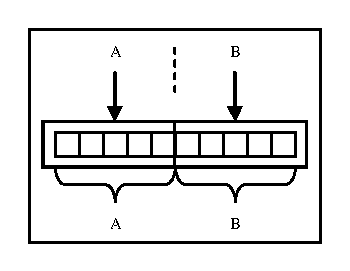
\includegraphics[scale=0.85]{Cells/cells-spatial-partition-explicit}
	\end{minipage}%
	\begin{minipage}[c]{0.5\linewidth}
		\centering 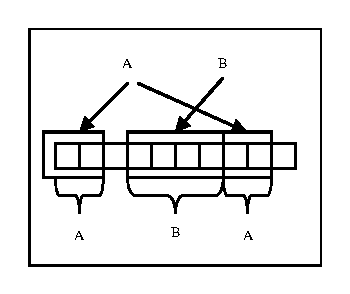
\includegraphics[scale=0.85]{Cells/cells-spatial-partition-implicit}
	\end{minipage}
	\caption{Depiction of the explicit versus implicit partitioning of input signals and the effects on the repertoire.}
	\label{pic:cells:spatial:explicit:v:implicit}
\end{figure}

%
% Empirical Study
%
\subsection{Spatial Repertoire Empirical Study}
%
% Aim
%
\subsubsection{Aim}
The aim of this investigation is to investigate cellular clonal selection constrained by a spatial repertoire structure. Toward this end, the study had the following goals:

\begin{enumerate}
	\item Investigate the effects on the repertoire composition and capability in adopting a spatial repertoire structures.
	\item Assess the effects on the repertoire in exploiting the spatial structure to localise clonal integration via replacement.
\end{enumerate}

%
% Method
%
\subsubsection{Method}

%
% Algorithms
%
\paragraph{Algorithms}
This study considers the Replacement Cellular Clonal Selection Algorithm (RCCSA), and two variations of the Spatial Cellular Clonal Selection Algorithm (SCCSA).
% RCCSA
The RCCSA defined in  Algorithm~\ref{alg:cells:realisation:algorithms:rccsa:exposure} was configured with $N_{cells}=100$, $N_{selected}=2$, and $N_{clones}=5$ to promote an allocation of ten cells per antigen in ACSP-10.
% SCCSA
Unlike RCCSA, SCCSA does not aggregate and integrate clones as a group into the repertoire, instead clones are replaced individually, with per-progenitor clonal sibling replacement exclusion. Two variations of the SCCSA algorithm were investigated: (1) a variation that organised the repertoire into a lattice although was constrained by the spatial organisation called holistic replacement (SCCSA-HR), and (2) a variation that exploited the spatial repertoire and constrained the integration of clones to the spatial neighbourhood of the progenitor cell and with exclusion of clonal siblings (like RCCSA and SCCSA-HR) called neighbourhood replacement (SCCSA-NR). The neighbourhood was defined as the square of the nine cells surrounding and including a given position in the toroidal lattice. Both SCCSA used the same configuration as RCCSA, although the lattice dimensions used the square root of $N_{cells}$ resulting in a 10-by-10 2-dimensional repertoire.

%
% Problems
%
\paragraph{Problems}
This study used the ACSP-10 problem used for the CCSA empirical study in Section~\ref{sec:cells:ccsa:ccsa}.

%
% Experiment
%
\paragraph{Experiment}
This study used the same experimental configuration including stop conditions, measures, as were used for the RCCSA empirical study in Section~\ref{sec:cells:ccsa:rcsa}, including the Average Best Matching Cells Per Antigen (ABMCPA). 
% new measures
An additional measure was used that calculated the average diversity of the 9-cell neighbourhood for each position in the lattice, called the Average Cell Neighbourhood Diversity (ACND). The diversity was calculated using the Average Cell Diversity (Equation~\ref{eq:cells:realisation:acd}) method for each neighbourhood, and averaged across all 100 neighbourhoods.

%
% Results
%
\subsubsection{Results}
% tables
Table~\ref{tab:cells:sccsa:study1} provides a summary of results for each algorithm-problem combination including the mean ($\bar{x}$) and standard deviation ($\sigma$) of collected measure values. The non-parametric Mann-Whitney~U statistical test was calculated pair-wise for all algorithms. 
% figures
Figures \ref{fig:cells:sccsa:study1:acd:boxplot}, \ref{fig:cells:sccsa:study1:ace:boxplot}, \ref{fig:cells:sccsa:study1:abmca:boxplot}, and \ref{fig:cells:sccsa:study1:acnd:boxplot} show the ACD, ACE, ABMCPA, and ACND on all algorithms respectively. 
% plots
Figure~\ref{fig:cells:sccsa:study1:plots} provides example plots of the state of the repertoire from the two spatial-based algorithms  (same configuration, random seeds of 1 and 5 for the algorithm and problem respectively). 

\begin{table}[htp]
	\centering\small
		\begin{minipage}{\textwidth}
		\begin{tabular}{llllllllll}
		\toprule
		\textbf{Problem} & \textbf{System} & \multicolumn{2}{c}{\textbf{ACD}} & \multicolumn{2}{c}{\textbf{ACE}} & \multicolumn{2}{c}{\textbf{ABMCPA}} & \multicolumn{2}{c}{\textbf{ACND}}\\
		\midrule
		\emph{ACSP} & \emph{CCSA} & $\bar{x}$ & $\sigma$ & $\bar{x}$ & $\sigma$ & $\bar{x}$ & $\sigma$ & $\bar{x}$ & $\sigma$\\
		\toprule
		ACSP-10 & RCCSA & 89.128 & 0.732 & 0.002 & 0.002 & 3.94 & 0.803 & N/A & N/A \\
		ACSP-10 & SCCSA-HR & 92.876 & 0.405 & 0.012 & 0.012 & 2.83 & 0.352 & 83.257 & 0.508 \\
		ACSP-10 & SCCSA-NR & 87.592 & 0.968 & 0.002 & 0.001 & 3.417 & 0.424 & 65.119 & 1.514 \\
		\multicolumn{2}{l}{\emph{Significant}} & True &  & True\footnote{False for RCCSA and SCCSA-NR} &  & True &  & True & \\
		\bottomrule
		\end{tabular}
		\end{minipage}
	\caption{Summary of results for SCCSA on AEP 10.}
	\label{tab:cells:sccsa:study1}
\end{table}


% graphs
\begin{figure}[htp]
	\subfloat[Average Cell Diversity (ACD) on ACSP-10.]{
	\label{fig:cells:sccsa:study1:acd:boxplot} %% label 
	\begin{minipage}[t]{0.50\textwidth}
		\centering 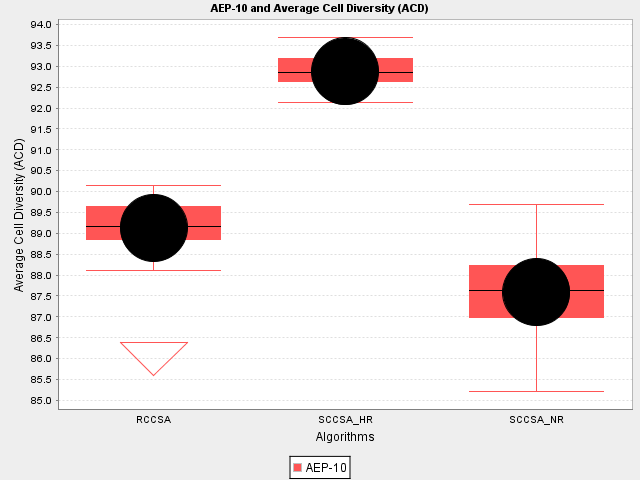
\includegraphics[scale=0.40]{Cells/SCCSA-ACD-plot}
	\end{minipage}}%
	%\hfill
	\subfloat[Average Cell Error (ACE) on ACSP-10.]{
	\label{fig:cells:sccsa:study1:ace:boxplot} %% label 
	\begin{minipage}[t]{0.50\textwidth}
		\centering 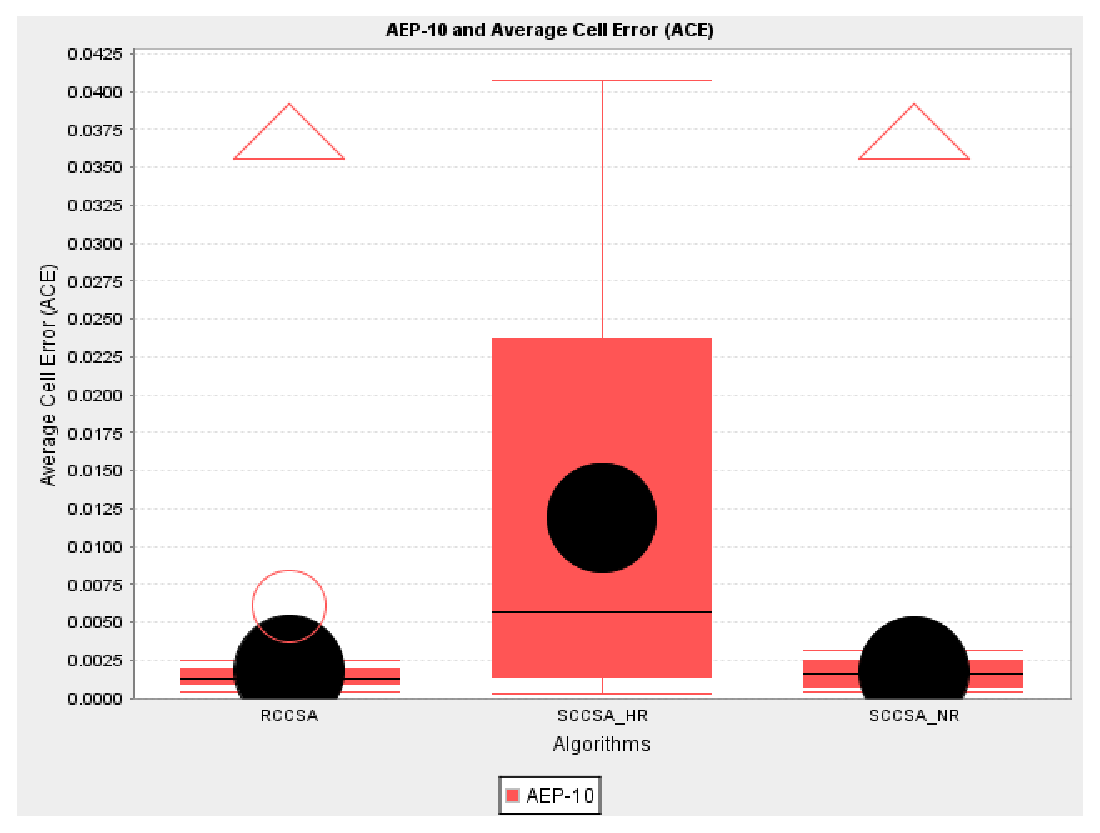
\includegraphics[scale=0.40]{Cells/SCCSA-ACE-plot}
	\end{minipage}}\\
	% new line for second set
	\subfloat[Average BMC Per Antigen on ACSP-10.]{
	\label{fig:cells:sccsa:study1:abmca:boxplot} %% label 
	\begin{minipage}[t]{0.50\textwidth}
		\centering 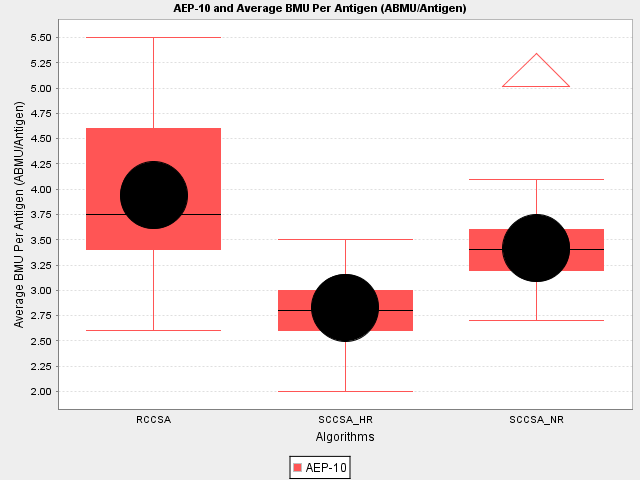
\includegraphics[scale=0.40]{Cells/SCCSA-ABMCPA-plot}
	\end{minipage}}%
	%\hfill
	\subfloat[Average Cell Neighbourhood Diversity on ACSP-10.]{
	\label{fig:cells:sccsa:study1:acnd:boxplot} %% label 
	\begin{minipage}[t]{0.50\textwidth}
		\centering 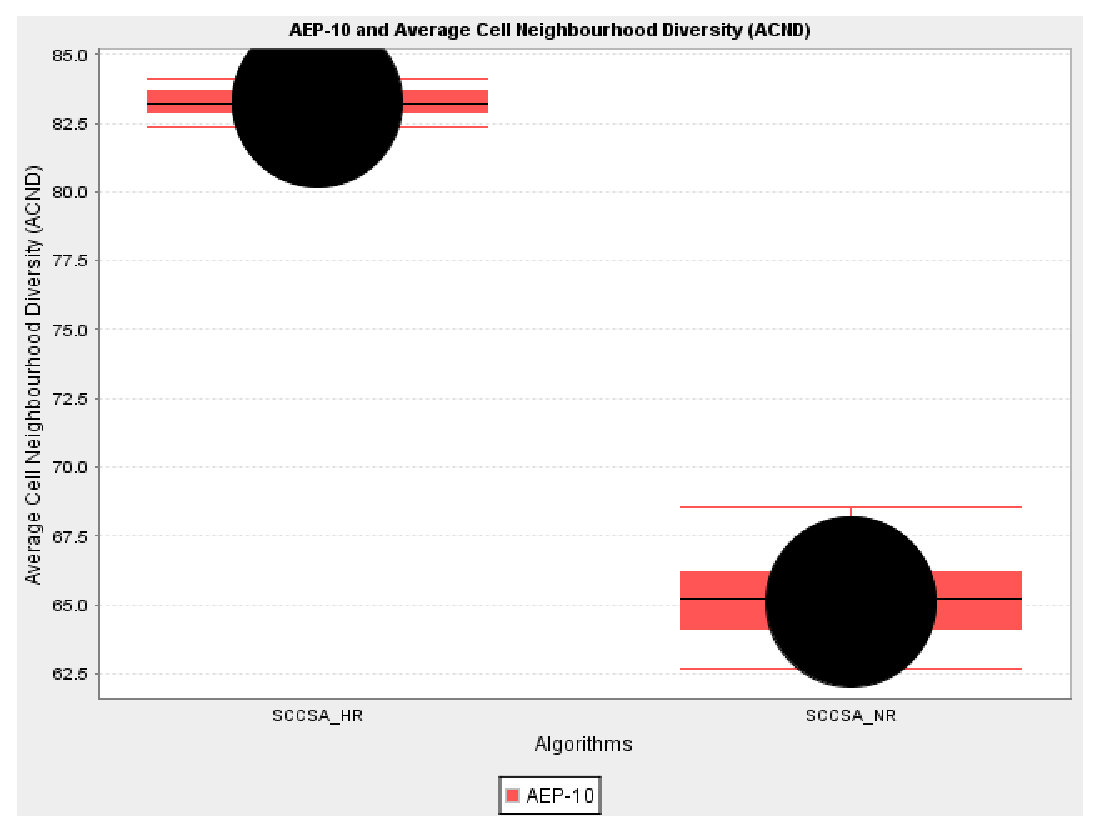
\includegraphics[scale=0.40]{Cells/SCCSA-ACND-plot}
	\end{minipage}}%
	\caption{Box-and-whisker plot's from the Spatial Repertoire Empirical Study.}
	\label{fig:tissues:sccsa:all:boxplot} %% label for entire figure
\end{figure}

% plots
\begin{figure}[htp]
	\subfloat[SCCSA-HR on ACSP-10.]{
	\label{fig:cells:sccsa:study1:a} %% label 
	\begin{minipage}[t]{0.50\textwidth}
		\centering 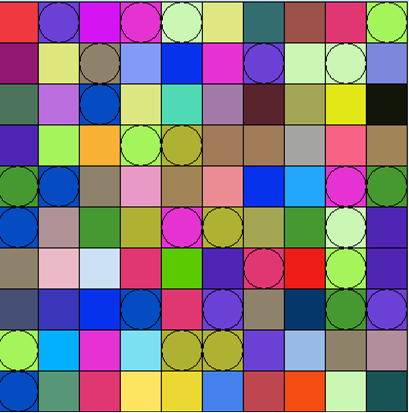
\includegraphics[scale=0.50]{Cells/SCCSA-HR-plot}
	\end{minipage}}%
	\hfill
	\subfloat[SCCSA-NR on ACSP-10.]{
	\label{fig:cells:sccsa:study1:b} %% label 
	\begin{minipage}[t]{0.50\textwidth}
		\centering 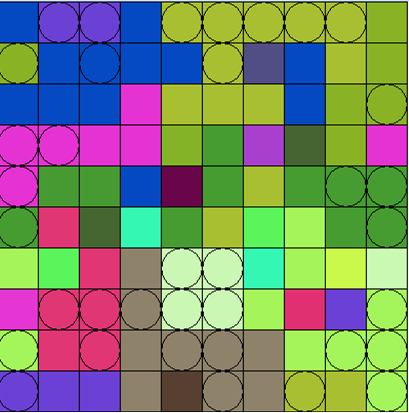
\includegraphics[scale=0.50]{Cells/SCCSA-NR-plot}
	\end{minipage}}\\
	% end
	\caption{Example plots of the spatial repertoire from two variations of SCCSA at the end of the run on ACSP-10 with BMC represented with circles.}
	\label{fig:cells:sccsa:study1:plots} %% label for entire figure
\end{figure}


%
% Analysis
%
\subsubsection{Analysis}
This section provides an analysis of the results reported in the previous section in the context of the goals of the empirical study. 

%
% Spatial Structure Trends
%
\paragraph{Spatial Structure Trends}
% section
This section considers the effects of storing the repertoire in a spatial structure by comparing the results of RCCSA to SCCSA with holistic replacement.
% measures
The use of the spatial structure in SCCSA-HR resulted in a small increase in repertoire diversity and in particular response error where ACE also showed a large increase in the variance of final ACE scores. The increase in diversity and error correlated with a decrease in the average number of BMC's.
The spatial structure was used in SCCSA-HR to hold the repertoire although was not exploited in any way. The difference in the repertoire composition and capability between the approach and RCCSA demonstrate the effect of the per-progenitor clonal set replacement used in SCCSA compared to the aggregated clonal set replacement in RCCSA.

%
% Localised Replacement Trends
%
\paragraph{Localised Replacement Trends}
% section
This section considers the exploitation of the spatial structure in the neighbourhood replacement used in SCCSA compared to holistic replacement.
% measures
The SCCSA-NR resulted in a the increased organisation of the repertoire as expected by localising cells for the same antigen into areas on the spatial repertoire structures. This was demonstrated by the decrease in repertoire diversity compared to both SCCSA-HR and RCCSA, and a small increase in ABMCPA compared to SCCSA-NR. Interesting the exploitation of spatial neighbourhood competition resulted in a ACE not significantly different from RCCSA, suggesting that such competition results in the same level of per-antigen specialisation within the repertoire as RCCSA. Importantly the increased organisation was demonstrated by the significant decrease in average repertoire diversity compared to holistic replacement, which was depicted in the example plot in Figure~\ref{fig:cells:sccsa:study1:plots} showing that this decrease was caused as a result of the clear grouping of similar cells (similar colours) in the spatial repertoire.

%
% Conclusions
%
\subsubsection{Conclusions}
This section summarises the findings of the empirical study into the Spatial Cellular Clonal Selection Algorithm in terms of the primitives that were the focus of the study and the expectations that motivated the study.

\begin{enumerate}
	\item Neighbourhood replacement provides intra-clone competition that results in similar general behaviours as consolidating the clone for replacement in RCCSA.
	\item Neighbourhood replacement results in the spatial localisation of clones on the lattice, the so called spatial responsibility effect as expected.
\end{enumerate}

%
% Response Mediation
%
\section{Response Mediation}
\label{sec:cells:mediated}
This section elaborates on the clonal selection by introducing a second repertoire of intermediate (mediator) cells to provide an adaptive context for localising the differential resource allocation of clonal selection, providing a model of decoupled \emph{feature detection} and \emph{system response}. 

%
% Mediated Clonal Selection
%
\subsection{Mediated Clonal Selection}
% metaphor
Two-signal theories have been proposed in immunology as verification signals permitting the proliferation and differentiation of lymphocytes. Historically developed for the activation of B-lymphocytes (in the context of self-nonself discrimination), the two-signal approach has also been extended to the various classes of T-cells. The dominant type of B-cell activation is dependant on Helper T-cells that identify MHC molecules on the surface of activated antigen-presenting B-cells. The detection of MHC provides a secondary verification signal to the B-cells, allowing them to proliferate and differentiate. This process is called the co-stimulation of B-cells by T-cells or T-cell dependant activation of B-cells. Likewise, T-cell activation requires an antigen specific signal via an antigen-presenting cell and a co-stimulating `antigen non-specific' verification signal. The theory of the two-signal activation of T-cells is called associative recognition theory \cite{Bretscher1970}.

% abstraction
\emph{Mediated Clonal Selection} or so-called inter-repertoire recognition decomposes the clonal selection process such that a mediation process is responsible for selecting those cells from the activated set that may proliferate. The mediation process is controlled by a sister repertoire of cells that also perform a clonal selection process using the activated cells of the first repertoire as input signals. The Helper T-cell metaphor is adopted such that the repertoire of cells (first repertoire) represents B-lymphocytes, which require a second verification signal from the helper T-lymphocytes (second repertoire) before proliferating and differentiating. After providing the secondary signal to the activated set of B-lymphocytes, the helper T-lymphocytes proceed with the cloning and maturation of the activated T-cells. Therefore, the T-cell repertoire is an application of the clonal selection algorithm that accepts the activated set of another clonal selection algorithm as a pseudo-`antigenic set'. Two concerns that must be reconciled in integrating the two repertoires are as follows: (1) The T-cells must select those B-cells from the B-cells activated set that may proliferate (2) The B-cell activated set provides multiple antigens simultaneously to the T-cell repertoire, to which it is possible to generate a T-cell activated set for each member of the B-cell activated set. The remainder of this section considers the implications of the second clonal selection governed repertoire from a variety of different perspectives.

% 
% Mapping Function
%
\subsubsection{Mapping Function}
% verification signal
The proliferation \emph{verification signal} for the activated B-cell's may be \emph{antigen-dependent} or \emph{antigen-independent}. If antigen-dependent, the information provided by the verification signal may be considered a generalisation of the input signals provided to the B-cell repertoire. If the verification signal is antigen-independent, then the information provided is a generalisation of the cells themselves in the B-cell repertoire. This is a subtle but potentially important difference that effects the representation of information by the system.

% about dependant
An antigen-dependent mapping from B-cell to T-cell requires that some regularities of the input signal are preserved. The transformation may be of the whole antigen itself, or just the part of the antigen recognised by the B-cell receptor. The T-cell repertoire adapts to a consistent (B-cell invariant) generalisation of the antigenic input patterns. An antigen-dependent mapping between the repertoires provides a top-down organisation of the relationship between the repertoires, where simply matching onto the second repertoire provides the verification signal.
% about independent
A potential concern with antigen dependence is that the mapping of the input patterns may be achieved in one repertoire, making the second repertoire redundant. An antigen-independent mapping disregards the regularities of the input signal, such that the T-cell is performing pattern recognition of B-cell receptors, rather than a pattern recognition of antigen (whether symbolic or sub-symbolic). The result is a T-cell repertoire that is developed independent of antigen, and dependent on the B-cell repertoire (which in turn develops in response to antigen). A potential concern with an antigen-independent mapping is that it is arbitrary such that T-cells are completely dependent on specific B-cell lineages, and regularity between B-cell patterns has no meaning other than ancestry (likely to make the mapping harder). 

%
% Formation of High-Order Structures
%
\subsubsection{Formation of High-Order Structures}
% general
Interestingly, the relationship between an antigen and cells, as well as cells between repertoires may be considered in the context of the formation and maintenance of higher-order structures.
% consider a single repertoire
For example in the case of a single repertoire, one antigen may map onto one cell providing a specialised mapping. This may be elaborated to include the extremes cardinality of relationship. For example, a one-to-many relationship between antigen and cells maybe considered a decomposition of feature extraction, particularly if the mapping is partial or sub-symbolic. Additionally, many antigen may be mapped onto many cells either directly (generalisation of one-to-one) or partially (cross reactivity), or onto a single cell, compressing the signal.

% consider relationships between repertoires
The relationship between repertoires adds a second level of complexity to the hierarchical structure. The same relationships apply although in this case between cells, with the importance difference that the relationships can be manipulated with mapping schemes, activated B-cell set size, and activated T-cell set size.
% control
For example, it may be desirable to coerce the B-cell repertoire to decompose antigen into regular features (many), and the T-cell receptor to generalise those features toward a specific meaning (few). Alternatively, the B-cell repertoire may be coerced to generalise (compress) based on common antigenic features (few), and the T-cell repertoire to decompose the B-cell information content into a variety of different meanings (many).

\begin{figure}[htp]
	\subfloat[Many-to-One.]{	
	\begin{minipage}[t]{0.50\textwidth}
		\centering 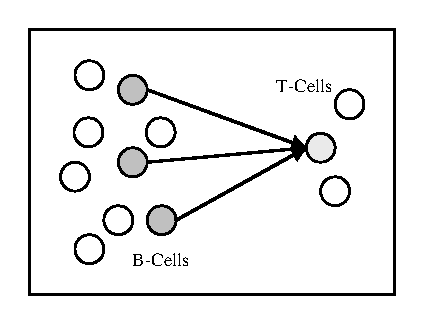
\includegraphics[scale=0.70]{Cells/mediated-many-to-one}
	\end{minipage}}%
	\hfill
	\subfloat[One-to-Many.]{	
	\begin{minipage}[t]{0.50\textwidth}
		\centering 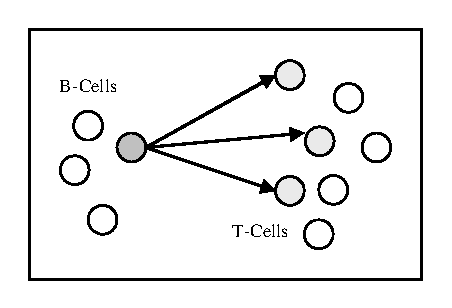
\includegraphics[scale=0.70]{Cells/mediated-one-to-many}
	\end{minipage}}\\
	% end
	\caption{Depiction of inter-repertoire structures based on the mapping of cells.}
	\label{fig:cells:mediated:structures} %% label for entire figure
\end{figure}

% altered activation scheme
Rather than treating each activated B-cell independently, the activated B-cells may interact with the T-cell population concurrently, such that multiple B-cells may activate a single T-cell. The T-cell repertoire may be configured such that a T-cell is required to match more than one B-cell before it may become activated. This provides a mechanism in which the T-cell repertoire facilitates the aggregation of multiple antigenic features into a single T-cell. The second repertoire facilitates the addition of a second layer of meaning. In the many-to-one case a T-cell may represent a high-order concept as an aggregate of multiple lower-level concepts (B-cells). The meaning is a single or small collection of concepts that are dependent on the presence of specific features (specific context). 
% examples
For example, \emph{Many-to-One} provides a consensus forming operation in which many lower-order concepts (such as extracted features) are aggregated together to form a high-order concept. The \emph{One-to-Many} relationship provides a descriptive operation in which a high-order concept is decomposed into a number of lower-order concepts (such as descriptive features). In both of these examples, the meaning implies a mapping that manages to preserve some regularities of the input signal, such that higher-order or lower-order concepts may be described. 

%
% Supervised Concept Formation
% 
\subsubsection{Supervised Concept Formation}
The incorporation of additional feedback into the algorithm allows an external process to assign meaning and supervise the mapping and formation of concepts. For the single repertoire algorithm, T-cell mediation provides an immunologically plausible basis for feedback (verification) to supervise the selection of activated receptor patterns in response to antigenic exposures. For the dual repertoire algorithm, tissue damage provides an immunologically plausible basis for feedback to supervise the selection of concepts formed in the T-cell repertoire, which in turn feeds back to the B-cell repertoire via the mediation process. The proposed integration of feedback results in two flows of information through the system. The top-down flow of antigenic signals results in B-cell receptors competing for activation, and T-cell receptors competing for activation of the B-cell receptor activated set. Those B-cells that receive the secondary signal, proliferate. The bottom-up flow of tissue-damage input results in T-cells competing for encouragement that the concepts that they represent are \emph{useful}. Those T-cells that receive a positive (non-negative, and perhaps non-neutral) feedback, proliferate. Therefore, the application of feedback (if available) is to the activated set of T-cells. In the absence of feedback, there is simply the absence of corrective behaviour: the punishment, or reward of the activated T-cell concept.


\begin{figure}[htp]
	\subfloat[Many-to-Few.]{	
	\begin{minipage}[t]{0.50\textwidth}
		\centering 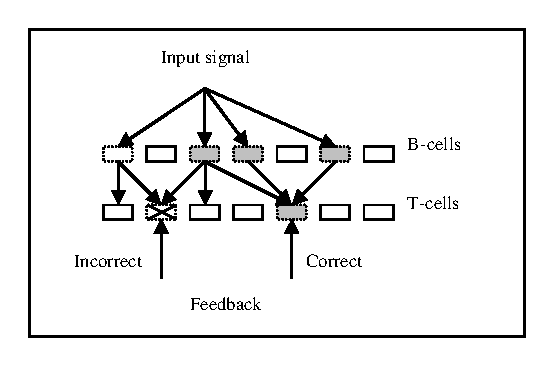
\includegraphics[scale=0.85]{Cells/mediated-many-to-few}
	\end{minipage}}%
	\hfill
	\subfloat[Few-to-Many.]{	
	\begin{minipage}[t]{0.50\textwidth}
		\centering 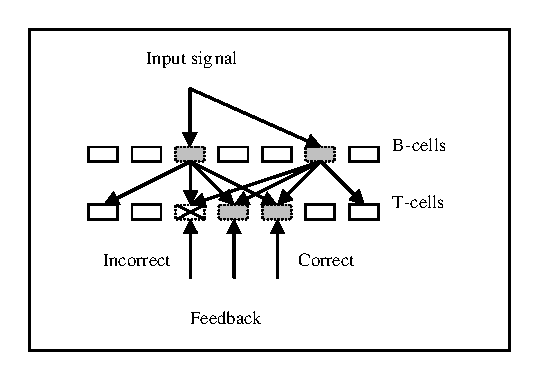
\includegraphics[scale=0.82]{Cells/mediated-few-to-many}
	\end{minipage}}\\
	% end
	\caption{Depiction of the integration of feedback for supervised structure formation.}
	\label{fig:cells:mediated:supervised} %% label for entire figure
\end{figure}

% on supervision
Bottom-up supervision of concept formation provides a natural agenda for investigating mediated clonal selection beyond the basic principles of mappings and structure formation and maintenance (for example, see Figure~\ref{fig:cells:mediated:supervised}). The integration of a feedback mechanism provide a natural relationship with the study of Reinforcement Learning (Section~\ref{subsec:cs:related:rl}).

%
% Mediated Empirical Study
%
\subsection{Mediated Empirical Study}
%
% Aim
%
\subsubsection{Aim}
The aim of this investigation was to asses the cellular clonal selection algorithm constrained by inter-cellular repertoire interactions. Toward this end, the study had the following goals:

\begin{enumerate}	
	\item Assess the behaviour of different inter-repertoire antigen-dependant mapping schemes.
	\item Investigate the effects of varied cellular cardinality in the relationships exploited via inter-repertoire mapping.
\end{enumerate}

%
% Method
%
\subsubsection{Method}

%
% Problems
%
\paragraph{Problems}
This study used the ACSP-10 problem used for the CCSA empirical study in Section~\ref{sec:cells:ccsa:ccsa}.

%
% Algorithms
%
\paragraph{Algorithms}
Algorithm~\ref{alg:cells:mediated:mccsa:exposure} defines the Mediated Cellular Clonal Selection Algorithm (ECCSA), where $Exposure(A, T)$ is a modified version of the $Exposure$ operation for RCCAS (defined in Algorithm~\ref{alg:cells:realisation:algorithms:rccsa:exposure}) that returns the selected set rather than the best matching cell. The RCCSA uses clonal sibling exclusion and a Hamming similarity function during replacement.

\begin{algorithm}[htp]
  \SetLine
  \SetKwData{Antigen}{A}
  \SetKwFunction{Exposure}{Exposure}
  \SetKwFunction{SelectBestMatchingCell}{SelectBestMatchingCell}
  
  \KwIn{\Antigen, $T_{bcells}$, $T_{tcells}$, $N_{bc-selection}$, $N_{bc-clones}$, $N_{tc-selection}$, $N_{tc-clones}$, $P_{mutation}$}
	\KwOut{$T_{rs}$}	
	
	$T_{rs} \leftarrow$0\;
	% expose the b cells
	$T_{bc-rs}$ = \Exposure{\Antigen, $T_{bcells}$, $N_{bc-selection}$, $N_{bc-clones}$, $P_{mutation}$}\;
	% expose the t cells
	$T_{tc-rs}$ = \Exposure{$T_{bc-rs}$, $T_{tcells}$, $N_{tc-selection}$, $N_{tc-clones}$, $P_{mutation}$}\;	
	% return it
	$T_{rs} \leftarrow$ \SelectBestMatchingCell{$T_{tc-rs}$}\;
	\Return{$T_{rs}$}\;
	\caption{Exposure Function for Mediated Cellular Clonal Selection.}
	\label{alg:cells:mediated:mccsa:exposure}
\end{algorithm}	

% mapping
The modified RCCSA \emph{Exposure} operation also permits the mapping of a selected set of cells ($T_{rs}$) to be treated as an antigen. This is achieved through use of an exposure operation that provides a mapping function that aggregates affinity for a given cell against a stimulating set of cells. The first part of this study considers two different examples of the mapping function: (1) Euclidean Mapping, and (2) Hamming Mapping. The affinity scores are aggregated within each cell of the repertoire against the stimulating set to provide a general indication of a cells capability against a stimulating set. In this part of the study, both the B-cell and T-cell repertoires used identical configurations as follows: $N_{cells}=100$,  $N_{selected}=1$, $N_{clones}=10$ (10\% of each repertoire per antigen).
% relationship
The second part of the study considered varied relationships between the two repertoires in terms of the size of the selected B-cell set which stimulates the T-cell repertoire, and the size of of the activated and responding T-cell set. A series of one-to-one and many-to-many relationships were assessed with the intermediates, where the number of clones and this repertoire assigned per antigen was kept constant at six (10\% of each repertoire per antigen) with regard to the selection size. The configurations are summarised in Table~\ref{tab:cells:mccsa:mappings:configuration}. A Euclidean mapping was used between the repertoires in this second part of the study.

\begin{table}[htp]
	\centering\small
		\begin{tabular}{lllllll}
		\toprule
		\textbf{Relationship} & \multicolumn{3}{c}{\textbf{B-Cells}} & \multicolumn{3}{c}{\textbf{T-Cells}} \\ 
		\midrule
		\emph{Name} & $N_{b-cells}$ & $N_{bc-selected}$ & $N_{bc-clones}$ & $N_{t-cells}$ & $N_{tc-selected}$ & $N_{tc-clones}$ \\ 
		\toprule
		\emph{1-to-1} & 60 & 1 & 6 & 60 & 1 & 6 \\ 
		\emph{1-to-N} & 60 & 1 & 6 & 60 & 6 & 1 \\ 
		\emph{N-to-1} & 60 & 6 & 1 & 60 & 1 & 6 \\ 
		\emph{N-to-N} & 60 & 6 & 1 & 60 & 6 & 1 \\ 
		\bottomrule
		\end{tabular}
	\caption{Summary of the configuration of the ECCSA with a series of inter-repertoire selection relationships.}
	\label{tab:cells:mccsa:mappings:configuration}
\end{table}

%
% Experiment
%
\paragraph{Experiment}
This study used the same general experimental configuration including stop conditions as were used for the CCSA empirical study in Section~\ref{sec:cells:ccsa:ccsa}. 
% new measures
A series of new measures were defined for the experiment. The Average Cell Diversity measure (defined in Equation~\ref{eq:cells:realisation:acd}) was calculated for each of the B-cell and T-cell repertoires referred to as the Average B-Cell Diversity (ABCD), and the Average T-Cell Diversity (ATCD) respectively. This treatment was performed to the Average Cell Error measure (defined in Equation~\ref{eq:cells:realisation:measure:ace}) referred to as the Average B-Cell Error (ABCE) and the Average T-Cell Error (ATCE) respectively, where the measure was taken as the best response from each repertoire against the antigen. The Average BMC per Antigen (defined in Equation~\ref{eq:cells:ccsa:rcca:abmcpa}) was adapted for the two re-repertoire configuration referred to as the Average Best Matching B-Cells Per Antigen (ABMBCPA) and the Average Best Matching T-Cells Per Antigen (ABMTCPA) respectively.
% system response
The system's response was taken as the best matching cell from the set of selected (activated) T-cells for each antigen exposure, called the Response Error (RE).
% mapping measure
A new measure was defined that calculated the T-cell error after mapping, averaged across each cell in the T-cell repertoire called the Average T-Cell Mapping Error (ATCME). This measure provided a general indication of the mapping error between the repertoire in the units of the specific mapping scheme used. The measure was also taken against just the set of T-cells activated and selected by the activated B-cells called the Average T-Cell Selected Set Mapping Error (ATCSSME).
% figure
Figure~\ref{fig:mccsa:measures} provides a depiction of the repertoires, the antigen, the selected sub-sets and the system response as well as how all the collected measures relate to these principle attributes of the ECCSA.

\begin{figure}[htp]
	\centering
		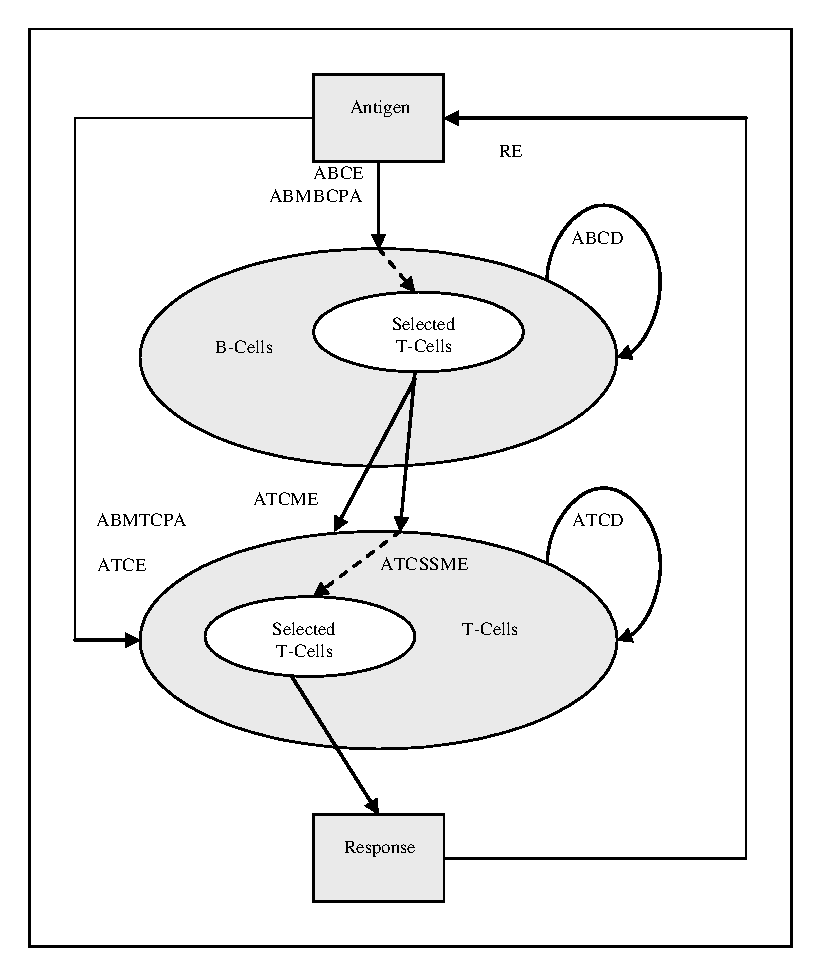
\includegraphics[scale=0.75]{Cells/MCCSA-measures}
	\caption{Depiction of the principle concerns of the MCCSA and the relationships in terms of the selected measures.}
	\label{fig:mccsa:measures}	
\end{figure}


%
% Results
%
\subsubsection{Results}
% tables
Table~\ref{tab:cells:mccsa:mappings} and Table~\ref{tab:cells:mccsa:relationships} provide a summary of results for each algorithm-problem combination including the mean ($\bar{x}$) and standard deviation ($\sigma$) of collected measure values. The non-parametric Mann-Whitney~U statistical test was calculated pair-wise for all algorithms. 
% mappings
%Figure~\ref{fig:cells:mccsa:study1:re:boxplot} shows RE, and Figure~\ref{fig:cells:mccsa:study1:plots} provide example plots for the mapping part of the study. 
% relationships 
Figures \ref{fig:cells:mccsa:study2:abcd:boxplot}, \ref{fig:cells:mccsa:study2:abce:boxplot}, \ref{fig:cells:mccsa:study2:atcd:boxplot}, \ref{fig:cells:mccsa:study2:atce:boxplot}, and \ref{fig:cells:mccsa:study2:re:boxplot} show the ABCD, ABCE, ATCD, ATCE, and RE respectively. Figure~\ref{fig:cells:mccsa:relationships:plots} provide example plots for all four configurations on the second relationship part of the study. 
% plots
Results from all example plots are taken from the end of the run with algorithm and problem configurations matching those used during experimentation, and a random number generator seed of 1 and 5 for the algorithm and problem respectively.

% comparison in the mappings
\begin{table}[htp]
	\centering\small
		\begin{tabular}{lllllc}
		\toprule
		\textbf{Measure} & \multicolumn{2}{c}{\textbf{Euclidean}} & \multicolumn{2}{c}{\textbf{Hamming}} & \textbf{Significant} \\ 
		\midrule
		 & $\bar{x}$ & $\sigma$ & $\bar{x}$ & $\sigma$ &  \\ 
		\toprule
		\emph{ABCD} & 89.399 & 0.822 & 89.399 & 0.822 & False \\ 
		\emph{ATCD} & 89.234 & 0.718 & 87.999 & 0.94 & True \\ 
		\emph{ABCE} & 0.003 & 0.002 & 0.003 & 0.002 & False \\ 
		\emph{ATCE} & 0.009 & 0.006 & 0.098 & 0.029 & True \\ 
		\emph{RE} & 0.009 & 0.006 & 0.617 & 0.123 & True \\ 
		\bottomrule
		\end{tabular}
	\caption{Summary of results for ECCSA with two different mapping schemes on ACSP-10.}
	\label{tab:cells:mccsa:mappings}
\end{table}

% figures of the mappings
%\begin{figure}[htp]
%	\centering
%		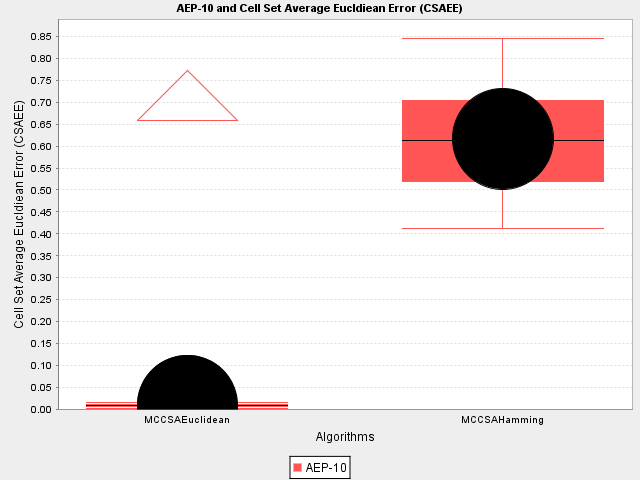
\includegraphics[scale=0.35]{Cells/MCCSA-Study1-MR}
%	\caption{Box-and-whisker plot of the Response Error of the two different mapping schemes on ACSP-10.}
%	\label{fig:cells:mccsa:study1:re:boxplot}
%\end{figure}

% plots of the mappings
\begin{figure}[htp]
	\subfloat[MCCSA-Euclidean on ACSP-10.]{
	\label{fig:cells:mccsa:study1:a} %% label 
	\begin{minipage}[t]{0.50\textwidth}
		\centering 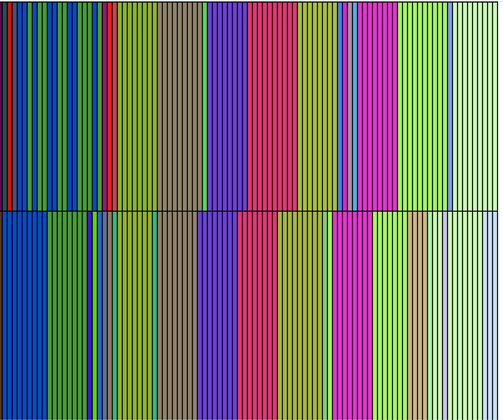
\includegraphics[scale=0.45]{Cells/MCCSAEuclidean-plot}
	\end{minipage}}%
	\hfill
	\subfloat[MCCSA-Hamming on ACSP-10.]{
	\label{fig:cells:mccsa:study1:b} %% label 
	\begin{minipage}[t]{0.50\textwidth}
		\centering 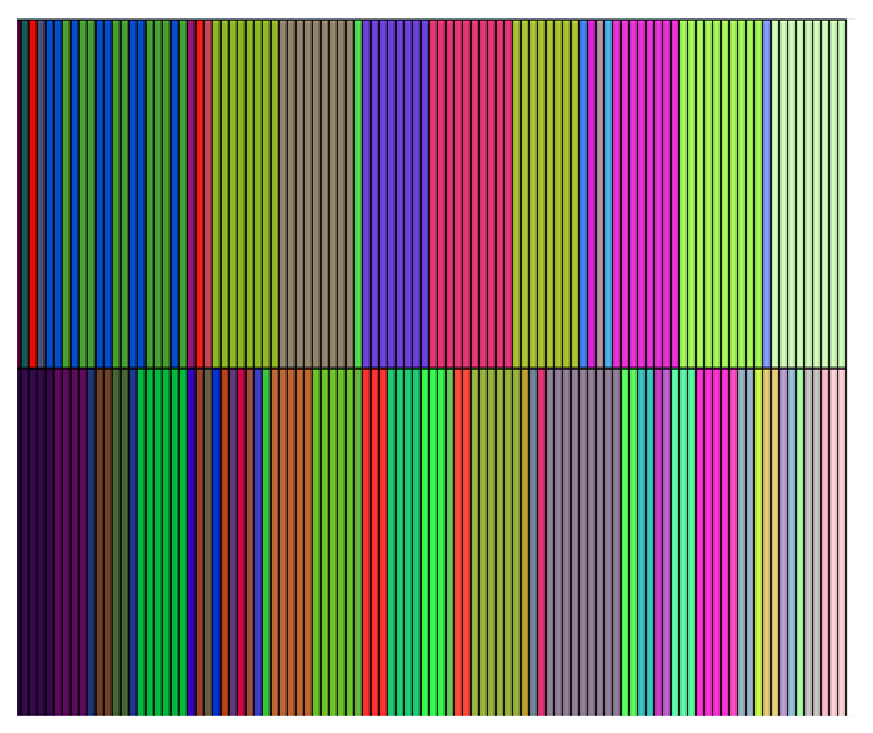
\includegraphics[scale=0.45]{Cells/MCCSAHamming-plot}
	\end{minipage}}\\
	% end
	\caption{Example plots of the B- (top of each plot) and T-Cell (bottom of each plot) repertoires from the ECCSA at the end of the run on ACSP-10 for two different inter-repertoire mapping types.}
	\label{fig:cells:mccsa:study1:plots} %% label for entire figure
\end{figure}


% relationships
\begin{table}
	\centering\small
		\begin{minipage}{\textwidth}
		\begin{tabular}{llllllllll}
		\toprule
		\textbf{Measure} & \multicolumn{2}{c}{\textbf{(1-1)}} & \multicolumn{2}{c}{\textbf{(1-N)}} & \multicolumn{2}{c}{\textbf{(N-1)}} & \multicolumn{2}{c}{\textbf{(N-N)}} & \textbf{Sig.} \\ 
		\midrule
		 & $\bar{x}$ & $\sigma$ & $\bar{x}$ & $\sigma$ & $\bar{x}$ & $\sigma$ & $\bar{x}$ & $\sigma$ &  \\ 
		\toprule
		\emph{ABCD} & 88.333 & 0.812 & 87.967 & 0.721 & 94.419 & 0.113 & 94.408 & 0.147 & True \\ 
		\emph{ATCD} & 88.005 & 0.755 & 94.298 & 0.146 & 88.103 & 0.924 & 94.309 & 0.105 & True \\ 
		\emph{ABCE} & 0.027 & 0.024 & 0.028 & 0.012 & 0.067 & 0.014 & 0.067 & 0.015 & True \\ 
		\emph{ATCE} & 0.052 & 0.021 & 0.076 & 0.015 & 0.102 & 0.019 & 0.093 & 0.013 & True \\ 
		\emph{ATCME} & 0.604 & 0.065 & 0.648 & 0.04 & 3.523 & 0.307 & 3.845 & 0.188 & True \\ 
		\emph{ATCSSME} & 0.042 & 0.02 & 0.158 & 0.023 & 0.844 & 0.129 & 1.161 & 0.121 & True \\ 
		\emph{ABMBCPA} & 2.713 & 0.33 & 3.13 & 0.426 & 1 & 0 & 1 & 0 & True\footnote{False for ECCSA(N-1) and ECCSA(N-N)} \\ 
		\emph{ABMTCPA} & 3.25 & 0.318 & 1 & 0 & 2.597 & 0.549 & 1 & 0 & True\footnote{False for ECCSA(1-N) and ECCSA(N-N)} \\ 
		\emph{RE} & 0.059 & 0.031 & 0.083 & 0.016 & 0.112 & 0.022 & 0.122 & 0.019 & True\footnote{False for ECCSA(N-1) and ECCSA(N-N)} \\ 
		\bottomrule
		\end{tabular}
		\end{minipage}
	\caption{Summary of results for ECCSA with four different inter-repertoire relationship schemes on ACSP-10.}
	\label{tab:cells:mccsa:relationships}
\end{table}

% figures of the relationships
\begin{figure}[htp]
	\subfloat[Average B-Cell Diversity (ABCD) on ACSP-10.]{
	\label{fig:cells:mccsa:study2:abcd:boxplot} %% label 
	\begin{minipage}[t]{0.50\textwidth}
		\centering 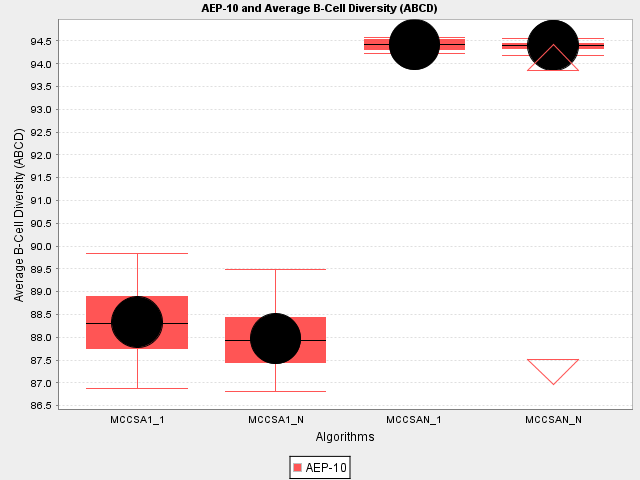
\includegraphics[scale=0.40]{Cells/MCCSA-relationships-ABCD}
	\end{minipage}}%
	%\hfill
	\subfloat[Average B-Cell Error (ABCE) on ACSP-10.]{
	\label{fig:cells:mccsa:study2:abce:boxplot} %% label 
	\begin{minipage}[t]{0.50\textwidth}
		\centering 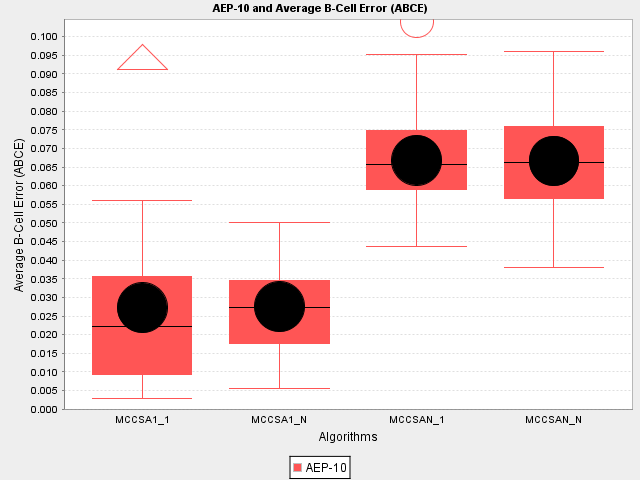
\includegraphics[scale=0.40]{Cells/MCCSA-relationships-ABCE}
	\end{minipage}}\\
	% new line for second set
	\subfloat[Average T-Cell Diversity (ATCD) on ACSP-10.]{
	\label{fig:cells:mccsa:study2:atcd:boxplot} %% label 
	\begin{minipage}[t]{0.50\textwidth}
		\centering 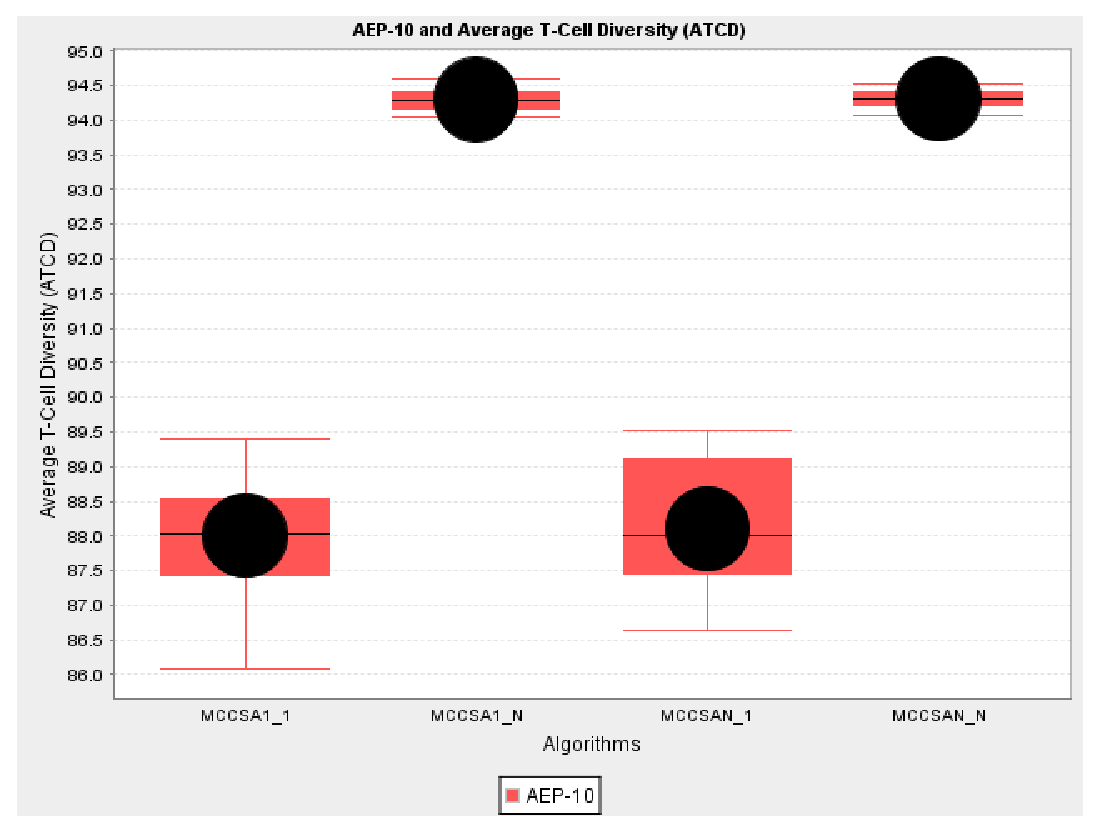
\includegraphics[scale=0.40]{Cells/MCCSA-relationships-ATCD}
	\end{minipage}}%
	%\hfill
	\subfloat[Average T-Cell Error (ATCE) on ACSP-10.]{
	\label{fig:cells:mccsa:study2:atce:boxplot} %% label 
	\begin{minipage}[t]{0.50\textwidth}
		\centering 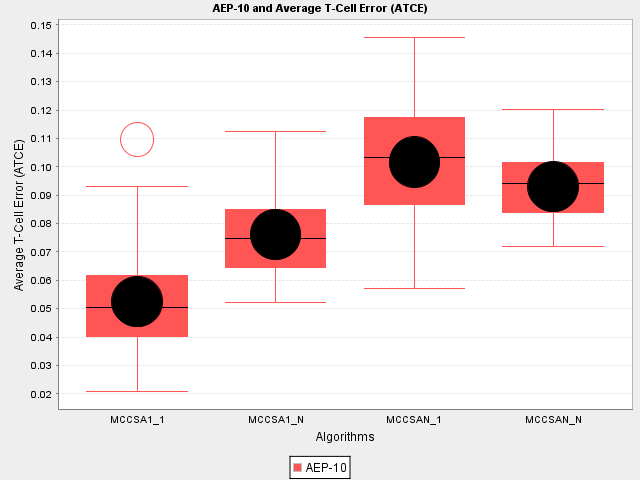
\includegraphics[scale=0.40]{Cells/MCCSA-relationships-ATCE}
	% new line for second set
	\end{minipage}}\\
	\subfloat[Response Error on ACSP-10.]{
	\label{fig:cells:mccsa:study2:re:boxplot} %% label 
	\begin{minipage}[t]{\textwidth}
		\centering 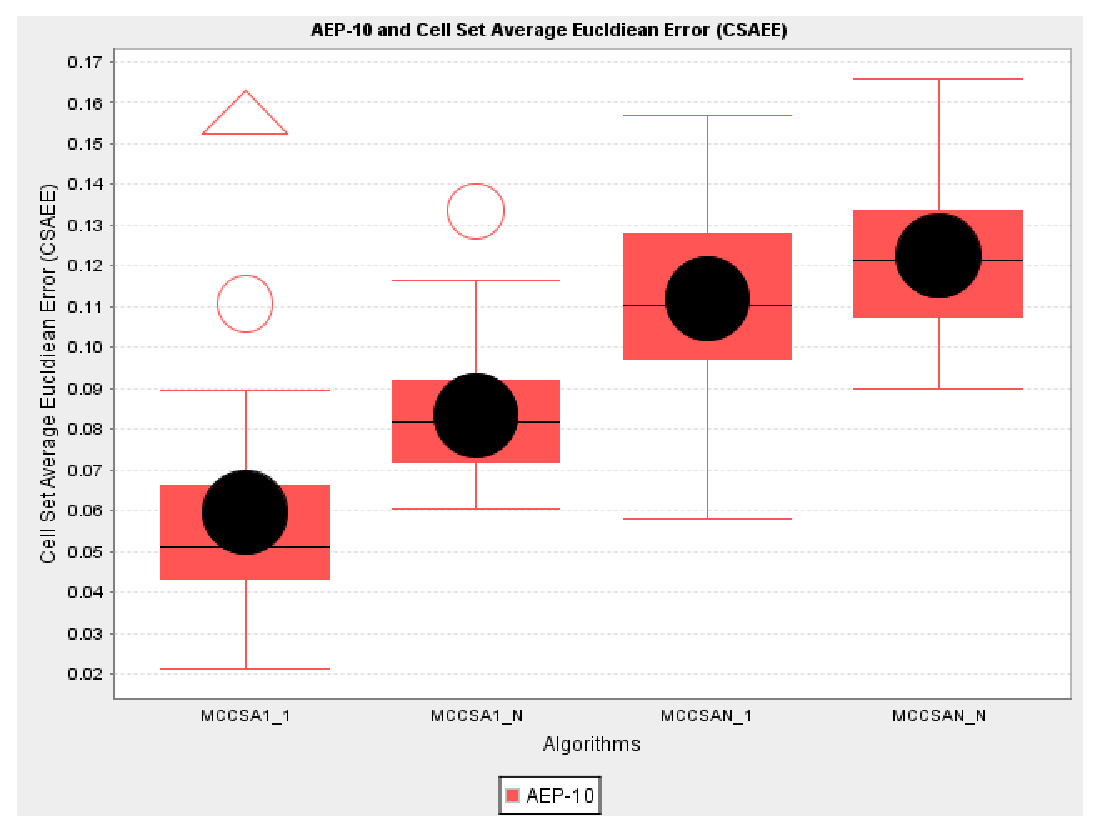
\includegraphics[scale=0.40]{Cells/MCCSA-relationships-RE}
	\end{minipage}}%	
	\caption{Box-and-whisker plot's for the relationship configuration with ECCSA.}
	\label{fig:cells:mccsa:all:boxplot} %% label for entire figure
\end{figure}


% plots of the relationships
\begin{figure}[htp]
	\subfloat[MCCSA(1-1).]{
	\label{fig:cells:mccsa:relationships:a} %% label 
	\begin{minipage}[t]{0.50\textwidth}
		\centering 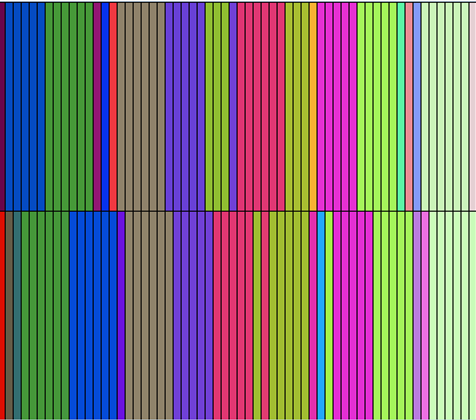
\includegraphics[scale=0.45]{Cells/MCCSA-1-1}
	\end{minipage}}%
	\hfill
	\subfloat[MCCSA(1-N).]{
	\label{fig:cells:mccsa:relationships:b} %% label 
	\begin{minipage}[t]{0.50\textwidth}
		\centering 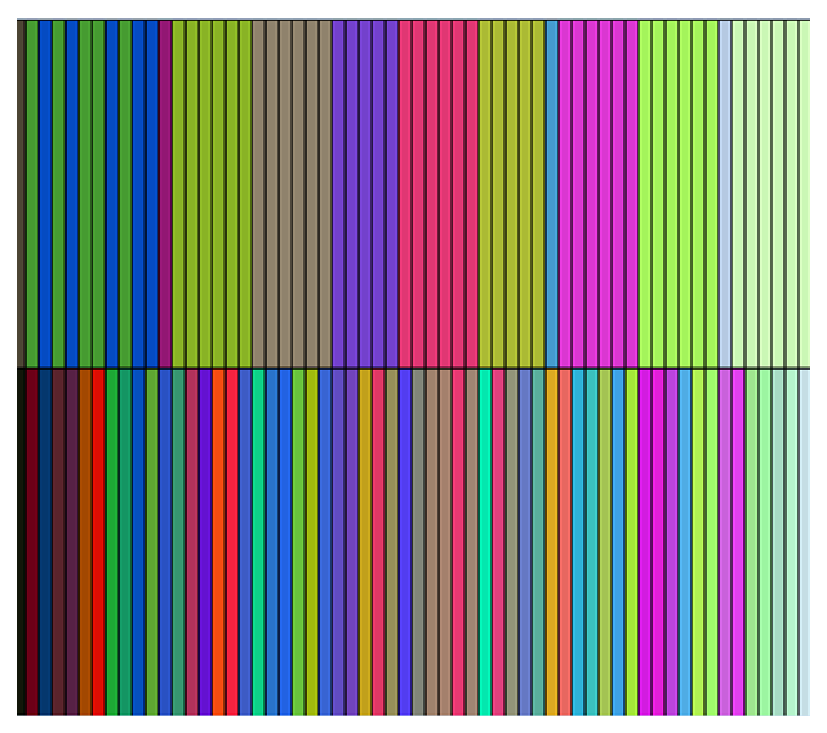
\includegraphics[scale=0.45]{Cells/MCCSA-1-N}
	\end{minipage}}\\
	% new line for second set	
	\subfloat[MCCSA(N-1).]{
	\label{fig:cells:mccsa:relationships:c} %% label 
	\begin{minipage}[t]{0.50\textwidth}
		\centering 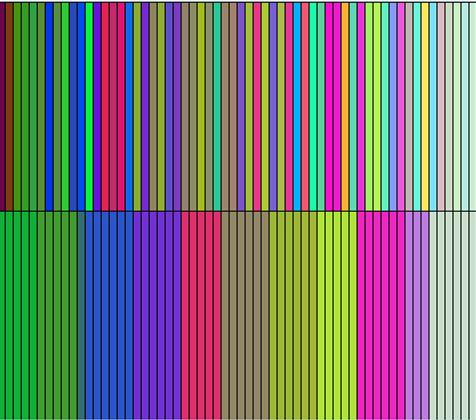
\includegraphics[scale=0.45]{Cells/MCCSA-N-1}
	\end{minipage}}%
	\hfill
	\subfloat[MCCSA(N-N).]{
	\label{fig:cells:mccsa:relationships:d} %% label 
	\begin{minipage}[t]{0.50\textwidth}
		\centering 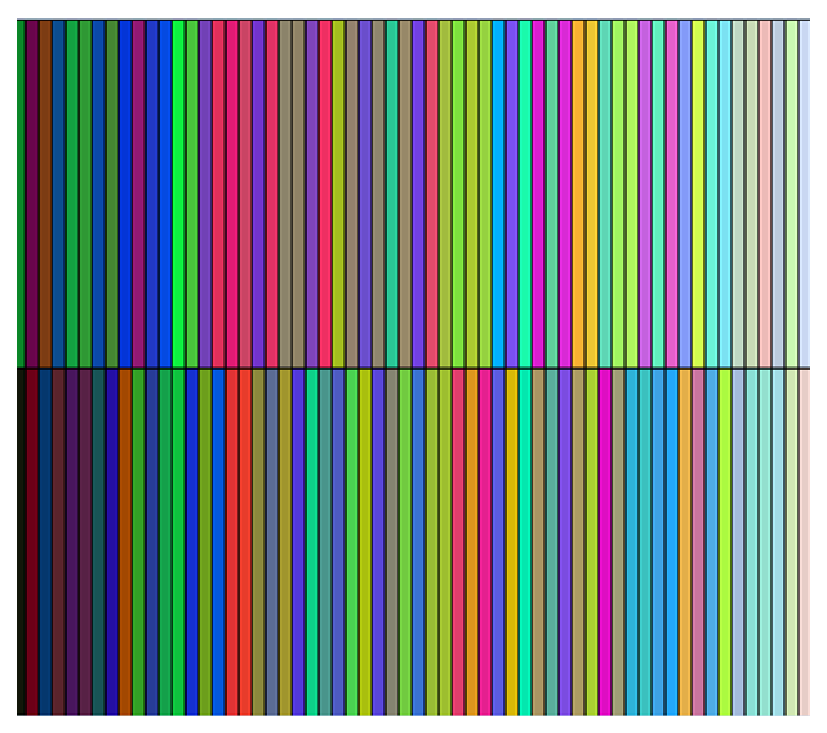
\includegraphics[scale=0.45]{Cells/MCCSA-N-N}
	\end{minipage}}
	% end
	\caption{Example plots of the B- (top of each plot) and T-Cell (bottom of each plot) repertoires from the MCCSA at the end of the run on ACSP-10 for all four inter-relationship types.}
	\label{fig:cells:mccsa:relationships:plots} %% label for entire figure
\end{figure}


%
% Analysis
%
\subsubsection{Analysis}
This section provides an analysis of the results reported in the previous section in the context of the goals of the empirical study. 

%
% Mapping Trends
%
\paragraph{Mapping Trends}
% section
This section considers the effects of using the Euclidean and Hamming antigen-dependant inter-repertoire schemes. 
% B-cells
The B-cell diversity and error show no significant difference between the mapping schemes. This is an expected result, as the mapping scheme and the chosen ECCSA does not effect the B-cell repertoire.
% T-cells
The T-cells showed a small decrease in diversity with the Hamming mapping, and more critically showed a factor of 10 increase in Average T-cell Error compared to the Euclidean mapping. This difference in error was reflected more strongly in the Response Error that showed a an increase in error of $\approx70$. 
% plots
The example plots in Figure~\ref{fig:cells:mccsa:study1:plots} clearly show well organised B-cell repertoires under both mapping schemes as expected, and the clear organisation and disorganisation in the T-cell repertoires between the Euclidean and Hamming schemes respectively.
% trends
These results demonstrate that under the circumstances investigated, that Hamming distance is not a sufficient approximation for Euclidean distance, not providing enough information to promote the same structures in the T-cell repertoire as were selected in the B-cell repertoire. These results demonstrate the fragility of proxy-based response to the antigen-centric mapping function. 

%
% Inter-Repertoire Relationship Trends
%
\paragraph{Inter-Repertoire Relationship Trends}
% section
This section considers the mapping relationships between the number of selected (stimulating) cells in each repertoire.
% b-cells and t-cells
The diversity and error of the B-cell repertoire increased with the number of selected B-cells. This same general behaviour was observed with the T-cell diversity and the number of selected T-cells. The ATCE increased with the number of selected T-cells with 1 triggering B-cell, although showed a small decrease with the increase in selected T-cells with $N$ selected T-cells.
% mapping
The average B-cell to T-cell mapping error showed an increase in the number of selected T-cells with both 1 and $N$ selected B-cells, and effect also observed with the mapping error of the selected T-cell set. 
% trend
Together these observations suggest that the selection of a single cell and integration of its clones results in a more specialised (lower diversity and error) repertoire and mapping. Conversely, the result suggests that the selection of a large activated set and integration of a few clones from each results in a more diverse cellular perspective on the cellular and/or antigenic trigger. 
% interpretation
This observation lends support to the \emph{oligoclonal axiom} of the clonal selection strategy outlined in Section~\ref{subsec:cells:paradigm:clonalselection}. More specifically, in the context of the replacement-based resource allocation scheme used in the assessed algorithms, selection and integration of few cells with many clones results in a more specific and less diverse repertoire. This finding in the context of the bi-repertoire model with antigenic and cellular triggers lends support to the same finding in Section~\ref{sec:cells:ccsa:rcsa}.
% error
This trend is observed poignantly in the Response Error from the relationship results where the 1-1 configuration achieved the lowest response-by-proxy error, increasing with the number of selected T-cells and selected B-cells. The plots in Figure~\ref{fig:cells:mccsa:relationships:plots} depict this in the organisation of the B-cell and T-cell repertoires in those configurations where a single cell is selected by antigen or cellular trigger resulting in the integration of a set of clonal siblings (1-1, 1-$N$, and $N$-1).


%
% Conclusions
%
\subsubsection{Conclusions}
This section summarises the findings of the empirical study into the Mediated Cellular Clonal Selection Algorithm in terms of the primitives that were the focus of the study and the expectations that motivated the study.

\begin{enumerate}
	% mappings
	\item \emph{Mappings}
	\begin{enumerate}		
			\item An antigen-centric mapping scheme results in the effective blind promotion (specialisation) of the T-cell repertoire and proxied response.
		\item The quality of the mapping with regard to proxied responses in mediated clonal selection is as good as the amount of antigen-centric information mapped between the repertoires. 
		\item The remapping of the antigen-assessment Euclidean distance resulted in an effective proxy response, whereas the approximation of the assessment in the Hamming distance resulted in a markedly unsuccessful proxied response.
	\end{enumerate}
	
	% relationships
	\item \emph{Relationships}
	\begin{enumerate}
		\item The number of activated B-cells and thus stimulus for the T-cell repertoire was an important factor in response capability, resulting in a specialisation of feature detectors for remapping.
		\item The one-to-one and one-to-many relationship configurations between the repertoires resulted in the better proxied responses, with more than a factor of two decrease in capability with an increase in the number of selected B-cells.
		\item One-to-Many selection and clonal integration for a given repertoire results in improved repertoire capability (lower error), increase repertories organisation (lower diversity), and an improved mapping given the specialisation it provides to the adaptive process.
	\end{enumerate}	
\end{enumerate}



%
% Cell-Cell Recognition
%
\section{Cell-Cell Recognition}
\label{sec:cells:network}
This section elaborates on clonal selection by introducing a pattern recognition interpretation of the Immune Network Theory and its integration into the cellular clonal selection framework.


%
% Network Clonal Selection}
%
\subsection{Network Clonal Selection}
\label{sec:cells:network:theory}
% metaphor
The Idiotypic Network Theory proposed by Jerne indicates that receptors (free or surface bound antibody) are selected by other receptors in addition to antigen (Section~\ref{subsec:background:negativeselection}). As such, one may define two additional types of receptor-to-receptor interaction in additional to conventional interaction with antigen: (1) The activation of a receptor by the idiotype of another receptor that results in the creation of more anti-receptor receptors, (2) The activation of a receptor that is specialised toward an antigen by another receptor that results in the creation of more receptors for the antigen without the presence of the antigen and anti-idiotype receptors for the triggering receptor. The theory suggests that the aggregation of these low-level behaviours results in a network of receptors that may interact with antigen and each other providing both an antigen-recognition system and the self-regulation of immune response. 


%
% Recognition and Relationships
%
\subsubsection{Recognition and Relationships}
The two direct receptor relationships include: \emph{Receptor-Antigen}: the traditional relationship where receptors for the antigen (target) are created with minor variations toward improving recognition, and \emph{Receptor-Receptor}: the the idiotypic relationship where receptors for the triggering receptor (target) are created (anti-receptor receptors) with minor variations toward improving recognition. Both of these cases provide examples of \emph{direct relationships}, that of a receptor and an antigen or a receptor and another receptor. In the first case, receptors have an \emph{implicit relationship} with other receptors that also match for the same antigen in that they compete with each other for selection by the antigen. The second case is a lot more interesting, given the recurrent relationships that may result. These relationships are considered in the context of how a given receptor came to be, assuming a single matching source is responsible for receptor maturation. For example, a receptor may match to another receptor that has been matured for an antigen. Therefore, there is a direct relationship between the first receptor and the second, as well as a \emph{proportional relationship} between the first receptor and the second receptors antigen (for example of both relationships see Figure~\ref{pic:cells:network:relationships:examples}). 

\begin{figure}[htp]
	\subfloat[Proportional Relationship.]{
	\label{pic:cells:network:relationships:examples:proportional} %% label for first subfigure
	\begin{minipage}[c]{0.5\linewidth}
		\centering 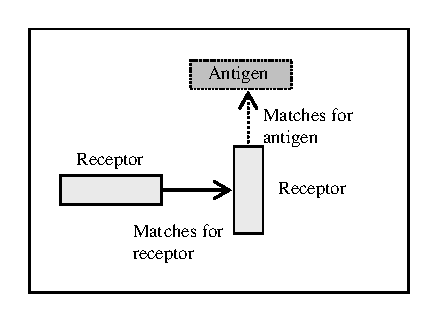
\includegraphics[scale=0.85]{Cells/network-relationships-proportional}
	\end{minipage}}%
	\hfill
	\subfloat[Implicit Relationship.]{
	\label{pic:cells:network:relationships:examples:implicit} %% label for second subfigure
	\begin{minipage}[c]{0.5\linewidth}
		\centering 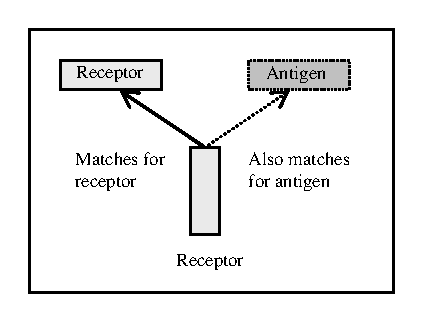
\includegraphics[scale=0.85]{Cells/network-relationship-implicit}
	\end{minipage}}
	\caption{Examples of more complex relationships that may be formed given receptor-receptor recognition.}
	\label{pic:cells:network:relationships:examples} %% label for entire figure
\end{figure}

%
% Matching Function
%
\subsubsection{Matching Function}
The clonal selection algorithm results in a repertoire that directly (relationship-wise) models features of the input space. When receptors themselves are treated as input signals a variety of representations may be used in the matching. The network theory proposes that receptors match onto a part of the receptor that is distinct for receptors of that lineage, although different from the receptors combining region (part of the other receptor that does the binding). A natural implementation scheme is to assign a random or remapping of the primary bit string to each \naive\ receptor that, like the primary string, is inherited and maturated by progeny cells. This results in the co-evolution (co-adaptation) of the primary string for activation and the secondary string for secondary effects (for example, see Figure~\ref{pic:cells:network:representation}).

\begin{figure}[ht]
	\centering
	\includegraphics[scale=0.85]{Cells/network-mapping-representation}
	\caption{Depiction of the two-string representation scheme.}
	\label{pic:cells:network:representation}
\end{figure}

A natural representation (using the same string for both) will likely result in a positive feedback system, where the exposed antigen will be amplified by repeated simulated exposures. Any regularity of the antigenic pattern that is provided on the secondary strings (such as sub-strings or reordering) will likely have this amplification effect, proportional to the fidelity of the mapping of the regularity. This amplification of input signal may be useful to reinforce the acquisition of knowledge. A natural representation will continue to promote the same instigating signal for as long as activated members are promoted to antigen-like status.

%
% Higher-Order Structures
%
\subsubsection{Higher-Order Structures}
A steady-state application of the approach emphasises some important properties regarding the formation of relationships as networks (graphs) of activation and exposure. In this interpretation, an antigen matches onto and activates a single receptor. The activated receptor is copied from the repertoire and is provided as an input signal in the next cycle. In this next cycle, both an antigen and the previously activated receptor are offered as input signals to the repertoire. A queue-based exposure scheme is used such that the more-recent activated receptors (instigation of relationship) are admitted, and older receptors are discarded. Therefore, the previously activated receptor is discarded, and the newly antigenic-activated cell is promoted to the next cycle as an input signal. The behaviour of this scheme may be described with an example (see Figure~\ref{pic:cells:network:recurrent} and Table~\ref{tab:cells:network:activationscheme}).

\begin{figure}[ht]
	\centering
	\includegraphics[scale=0.85]{Cells/network-structures-feedback}
	\caption{Example of a simple two-receptor promotion scheme.}
	\label{pic:cells:network:recurrent}
\end{figure}

\begin{table}[ht]
	\centering\small
		\begin{tabular}{lll}
		\toprule
		\textbf{Cycle} & \textbf{Exposed} & \textbf{Activated} \\ 
		\toprule
		$1$ & A1 & R1 \\ 
		\midrule
		$2$ & A2, R1 & R2, R1a \\ 
		\midrule
		$3$ & A3, R2 & R3, R2a  \\ 
		\midrule
		$4$ & A4, R3 & R4, R3a \\ 
		\midrule
		$t$ & $A_t$, $R_{t-1}$ & $R_t$, $R_{t-1}a$ \\ 
		\bottomrule
		\end{tabular}	
	\caption{Exposure-activation scheme for a minimal implementation.}
	\label{tab:cells:network:activationscheme}
\end{table}

If a natural mapping is used for $string2$, then the scheme provides a simple signal-reinforcement scheme that provides a linear amplification ($t-1$) reinforcement of signals past. If a remapping scheme is used for $string2$ (such as a random string), then the scheme provides new information in subsequent exposures that may result in the formation of a connection between two different input signals. The simplest example is the selection of $R1a$ by $A2$. In a natural mapping, if $A2$ selected $R1a$ then $A1$ and $A2$ would be the same input signal, and $R1$ and $R1a$ are likely the same receptor or clonal siblings (same ancestor). In a remapping scheme (such as random), it is possible for the remapped string to match for a receptor that is also matched for by an antigen (see Figure~\ref{pic:cells:network:remapping}). 

\begin{figure}[ht]
	\centering
	\includegraphics[scale=0.85]{Cells/network-remapping-schemes}
	\caption{Depiction of the example difference between a natural and remapping scheme.}
	\label{pic:cells:network:remapping}
\end{figure}

The remapping example provides an example of a relationship that may form between two different antigen ($A1$ and $A2$), facilitated by the remapping of receptors using the two-string scheme. If $A2$ is withdrawn, the relationship is fostered by $A1$, which activates $R1$, which in turn activates $R1a$. If $A2$ is withdrawn for all time, then the relationship will deteriorate due to genetic drift\footnote{The relationship is fostered by activation (usefulness), although here genetic drift refers to the adaptation of receptors (their progeny) in response to activation.}, thus $A2$ provides a correcting influence to the relationship. If $A1$ is withdrawn then the other half of the relationship is reinforced ($R1a$), and again if $A1$ is not returned, then $R1a$ may drift such that R1 does not match to it any longer. The example relationship is unidirectional, in that the primary string of $R1a$ is a generalisation of $A2$ and $R1$'s secondary string. A natural extension is to consider the implications of $R1a$'s secondary string. If $R1a$ matches for $R1$ then both $R1$ and $R1a$ provides surrogates for $A1$ and $A2$ reinforcing each other and the repertoires relationship between $A1$ and $A2$. It requires that $R1$'s primary string is a generalisation of $A1$ and $R1$'s secondary string. This network may be depicted as follows ($R1a$ is renamed $R2$).

\begin{figure}[ht]
	\centering
	\includegraphics{Cells/network-remapped-example}
	\caption{Depiction of the relationship between remapped antigen and receptors ($ps$ is primary and $ss$ is secondary string).}
	\label{pic:cells:network:remappingspecific}
\end{figure}

A larger queue allows more intra-antigen relationships (larger relationship structures in general), which in turn may prolong the activation of structures, but does not facilitate perpetual (antigen-independent) structure formation. Therefore, \emph{Structure Durability} is defined when the exposure set size defines the sustainability of a structure in active memory (essentially defining short-term memory), in the absence of renewed promotion. Finally, the examples do not take into account the proliferation of selected receptors, therefore the density concerns were subsumed with activation counts that delineated receptor persistence. Additionally, in the structures proposed the secondary strings become surrogates for antigen strings, thus `take the form' of antigen signals. This suggests that a mapping, such as substring's or reordering of the primary string may be easier for the system to retrofit for such a purpose rather than a random-based mapping (assuming similarity rather than complementarity of the mapping between receptors and antigen).

%
% Recurrent Empirical Study
%
\subsection{Recurrent Empirical Study}
\label{sec:cells:network:recurrent:study}
%
% Aim
%
\subsubsection{Aim}
The aim of this empirical study is to investigate some of the primiting behaviours of the cellular clonal selection strategy with intra-repertoire (network) interactions, specifically the recurrent network model. Toward this end, the study had the following motivating goals:

\begin{enumerate}	
	\item Investigate the effects on the composition and capability of the repertoire under recurrent cellular exposures.
	\item Assess a variety of cell promotion pressures in the recurrent network model.
\end{enumerate}

%
% Method
%
\subsubsection{Method}

%
% Problems
%
\paragraph{Problems}
This study used the ACSP-10 problem used for the CCSA empirical study in Section~\ref{sec:cells:ccsa:ccsa}.

%
% Algorithms
%
\paragraph{Algorithms}
Algorithm~\ref{alg:cells:nccsa:recurrent} defines the recurrent variation of the Network Cellular Clonal Selection Algorithm. Like ECCSA, two exposures occur each epoch, although unlike ECCSA both exposures occur to the same repertoire of cells. The second exposure involves the exposure of the Best Matching Cell (BMC) from the last \emph{antigen} exposure ($BMC_{t-1}$) to the repertoire. A cellular exposure involves the assessment of the repertoire against the representation in the cell, specifically using the Euclidean affinity function between the representation as is used between an antigen and a cell (defined in Equation~\ref{eq:cells:realised:euclidean}).

\begin{algorithm}[htp]
  \SetLine
  \SetKwData{Tissue}{T}
  \SetKwData{Antigen}{A}
  \SetKwFunction{Exposure}{Exposure}
  \KwIn{\Antigen, \Tissue, $BMC_{t-1}$, $N_{selection}$, $N_{clones}$, $P_{mutation}$}
	\KwOut{$T_{rs}$}	
	
	% expose to the antigen
	$T_{rs} \leftarrow$ \Exposure{\Antigen, \Tissue, $N_{selection}$, $N_{clones}$, $P_{mutation}$}\;		
	% expose to the last bmu
	\Exposure{$BMC_{t-1}$, \Tissue, $N_{selection}$, $N_{clones}$, $P_{mutation}$}\;	
	% return it	
	\Return{$T_{rs}$}\;
	
	\caption{Recurrent Network Cellular Clonal Selection.}
	\label{alg:cells:nccsa:recurrent}
\end{algorithm}	

% natural mapping
A Natural Mapping variation of the approach was assessed to provide a baseline of performance referred to as RE-NCCSA-NM. The algorithm responded to each exposure using the replacement mechanisms of RCCSA, and used the following configuration: $N_{cells}=100$, $N_{selected}=1$, and $N_{clones}=5$, assigning 5\% of the repertoire per exposed stimulus. This approach was called natural mapping, because indeed no mapping was used, where $BMC_{t-1}$ were exposed directly to the repertoire, likely causing their clonal siblings in the repertoire to respond.
% remapped
A remapping approach was used where each cell was provided with two data strings: a primary string which responded to exposed stimuli, and a secondary string which may be used as an antigenic stimulus (the two-string method described in Section~\ref{sec:cells:network:theory}).
% configuration
Table~\ref{tab:network:nccsa:renccsa} defines a set of four different \emph{replacement-based} promotion schemes used with the mapping variation of the algorithm. The schemes are replacement based in that the configurations define the specific pressures applied during the competition for limited position in the repertoire during the integration of clones. \emph{Similarity} refers to the specific representation of cells (primary or secondary) used to match clones with cells in the repertoire, and \emph{Assessment} refers to the affinity scoring (against the primary or secondary string) used during the tournament for the position in the repertoire between a clone and its most similar counterpart in the repertoire.
% expectations
The promotion of the antigen in the secondary representation is expected to promote similar cells in the recurrent exposure. The promotion of the cellular stimulus in the primary representation in the cellular exposure is expected to improve the mapping in the recurrent exposure. 

\begin{table}[htp]
	\centering\small
		\begin{tabular}{lllll}
		\toprule
		\textbf{R-NCCSA} & \multicolumn{2}{c}{\textbf{Antigen Exposure}} & \multicolumn{2}{c}{\textbf{Cellular Exposure}} \\ 
		\midrule
		\emph{Name} & \emph{Assessment} & \emph{Similarity} & \emph{Assessment} & \emph{Similarity} \\ 
		\toprule
		\emph{PP} & Primary  & Primary  & Primary  & Primary  \\ 
		\emph{PS} & Primary  & Primary  & Secondary & Secondary \\ 
		\emph{SS} & Secondary & Secondary & Secondary & Secondary \\ 
		\emph{SP} & Secondary & Secondary & Primary  & Primary  \\ 
		\bottomrule
		\end{tabular}
	\caption{Summary of the various replacement configurations for the mapped Recurrent Exposure Network Cellular Clonal Selection Algorithm (RE-NCCSA).}
	\label{tab:network:nccsa:renccsa}
\end{table}


%
% Experiment
%
\paragraph{Experiment}
This study used the same general experimental configuration including stop conditions as were used for the CCSA empirical study in Section~\ref{sec:cells:ccsa:ccsa}. 
% new measures
Two additional diversity measures were introduced to assess the composition of the repertoire with regard to secondary mappings. The Average Cell Mapped Diversity (ACMD) assesses the average Hamming distance of a given cell to all the other cells in the repertoire with regard to the secondary representation. The Average Network Cell Diversity (ANCD) provided a similar diversity measure although treats both representations of a given cell as one providing an indication of the composition of the repertoire independent of representations. Both diversity measures use the same mechanism as ACD in Equation~\ref{eq:cells:realisation:acd} on their representations respectively. Finally, a measure was introduced to assess the state of the mappings between the repertoire and recurrent cellular exposures called the Average Mapped Best Matching Cell Error (AMBMCE), that averaged the Euclidean distance between recurrent cells secondary representation and the BMC in the repertoire for each epoch using the same mechanism as ACE in Equation~\ref{eq:cells:realisation:measure:ace}.

%
% Results
%
\subsubsection{Results}
% tables
Table~\ref{tab:network:nccsa:rnccsa:results} provide a summary of results for each algorithm-problem combination including the mean ($\bar{x}$) and standard deviation ($\sigma$) of collected measure values. The non-parametric Mann-Whitney~U statistical test was calculated pair-wise for all algorithms. 
% graphs
Figures \ref{fig:cells:network:rnccsa:ace:boxplot}, \ref{fig:cells:network:rnccsa:acd:boxplot}, \ref{fig:cells:network:rnccsa:ambmue:boxplot} show the ACE, ACD, and AMBMCE respectively. 
% plots
Figure~\ref{fig:cells:nccsa:rnccsa:plots} provide example plots of the response mapping and final repertoire. Results from all example plots are taken from the end of the run with algorithm and problem configurations matching those used during experimentation, and a random number generator seed of 1 and 5 for the algorithm and problem respectively.

\begin{table}[htp]
	\centering\small
		\begin{minipage}{\textwidth}
		\begin{tabular}{lllllllllll}
		\toprule
		\textbf{System} & \multicolumn{2}{c}{\textbf{ACD}} & \multicolumn{2}{c}{\textbf{ACE}} & \multicolumn{2}{c}{\textbf{ACMD}} & \multicolumn{2}{c}{\textbf{ANCD}} & \multicolumn{2}{c}{\textbf{AMBMCE}}\\
		\midrule
		\emph{NCCSA} & $\bar{x}$ & $\sigma$ & $\bar{x}$ & $\sigma$ & $\bar{x}$ & $\sigma$ & $\bar{x}$ & $\sigma$ & $\bar{x}$ & $\sigma$\\
		\toprule
		NM & 93.218 & 0.248 & 0.019 & 0.011 & N/A & N/A & N/A & N/A & 0 & 0 \\
		PP & 91.974 & 0.413 & 0.09 & 0.025 & 91.777 & 0.46 & 183.751 & 0.669 & 0.184 & 0.026 \\
		PS & 91.912 & 0.31 & 0.03 & 0.013 & 92.032 & 0.453 & 183.944 & 0.597 & 0.173 & 0.025 \\
		SS & 91.805 & 0.429 & 0.211 & 0.04 & 91.783 & 0.419 & 183.588 & 0.609 & 0.147 & 0.034 \\
		SP & 91.744 & 0.421 & 0.234 & 0.039 & 91.745 & 0.403 & 183.489 & 0.542 & 0.162 & 0.03 \\
		\emph{Sign.} & True &  & True &  & True\footnote{False for RNCCSA-PP and RNCCSA-SS, RNCCSA-PP and RNCCSA-SP, RNCCSA-SS and RNCCSA-SP} &  & True\footnote{False for RNCCSA-PP and RNCCSA-PS, RNCCSA-PP and RNCCSA-SS, RNCCSA-PP and RNCCSA-SP, RNCCSA-SS and RNCCSA-SP} &  & True\footnote{False for RNCCSA-PP and RNCCSA-PS, RNCCSA-PS and RNCCSA-SP, RNCCSA-SS and RNCCSA-SP} & \\
		\bottomrule
		\end{tabular}	
		\end{minipage}
	\caption{Summary of results for Recurrent Network Cellular Clonal Selection Algorithm (R-NCCAS) on ACSP-10}
	\label{tab:network:nccsa:rnccsa:results}
\end{table}

% graphs
\begin{figure}[htp]
	\subfloat[Average Cell Error on ACSP-10.]{
	\label{fig:cells:network:rnccsa:ace:boxplot} %% label 
	\begin{minipage}[t]{0.50\textwidth}
		\centering \includegraphics[scale=0.41]{Cells/RNCCSA-ACE-plot}
	\end{minipage}}%
	\hfill
	\subfloat[Average Cell Diversity on ACSP-10.]{
	\label{fig:cells:network:rnccsa:acd:boxplot} %% label 
	\begin{minipage}[t]{0.50\textwidth}
		\centering \includegraphics[scale=0.41]{Cells/RNCCAS-ACD-plot}
	\end{minipage}}\\
	%\hfill
	\subfloat[ Average Mapped BMC Error on ACSP-10.]{
	\label{fig:cells:network:rnccsa:ambmue:boxplot} %% label 
	\begin{minipage}[t]{\textwidth}
		\centering \includegraphics[scale=0.41]{Cells/RNCCSA-AMBMUE-plot}
	\end{minipage}}%
	\caption{Box-and-whisker plot's from the Recurrent NCCSA Empirical Study.}
	\label{fig:cells:nccsa::study1:all:boxplot} %% label for entire figure
\end{figure}


% plots of PS
\begin{figure}[htp]
	\subfloat[Response Mapping plot for R-NCCSA-PS, shows $A$, $BMC_{t1}a$, $BMC_{t-1}$, $BMC_{t1}b$ from left to right, for an epoch.]{
	\label{fig:cells:nccsa:rnccsa:a} %% label 
	\begin{minipage}[t]{0.45\textwidth}
		\centering \includegraphics[scale=0.45]{Cells/RNCCSA-PS-map-plot}
	\end{minipage}}%
	\hfill
	\subfloat[Repertoire plot for R-NCCSA-PS, shows primary and secondary representations and antigen from left to right.]{
	\label{fig:cells:nccsa:rnccsa:b} %% label 
	\begin{minipage}[t]{0.45\textwidth}
		\centering \includegraphics[scale=0.45]{Cells/RNCCSA-PS-rep-plot}
	\end{minipage}}\\
	% end
	\caption{Example plots from of the response mappings and final repertoire from R-NCCSA-PS on ACSP-10.}
	\label{fig:cells:nccsa:rnccsa:plots} %% label for entire figure
\end{figure}


%
% Analysis
%
\subsubsection{Analysis}
This section provides an analysis of the results reported in the previous section in the context of the goals of the empirical study. 

%
% Promotion Trends
%
\paragraph{Promotion Trends}
% this section
This section considers the results of the recurrent network algorithm in the context of the trends for the different promotion schemes.
% generally
The natural mapping achieved the best results with regard to ACE as expected, showing a AMBMCE of zero suggesting that cells mapped onto themselves or clonal siblings with no error on average by the end of the run, providing an ideal (in the mapping sense) case for comparison.
% diversity
The various promotion schemes for the mapped recurrent algorithm showed little comparative difference between the three diversity scores: ACD, ACMD, and ANCD. The ACD scores showed a slight decrease with the remapping approaches compared to the natural mapping. The similarity between ACD and ACMD scores suggests that organisation of the information in the primary and secondary representations (pseudo-repertoires) was generally equivalent across the promotion schemes.
% ACE
The telling results were provided in the error measures. The two promotion schemes that promoted the primary representation achieved a much lower ACE as expected than those that promoted the secondary representation against the antigen. Interestingly the configuration that promoted the secondary representation against the cellular exposure (PS) performed better than the promotion of the primary string on both exposures (PP). 
% AMBMCE
The error results for the recurrent cellular exposures were poor compared to error scores for viable ACSP ($<0.1$), where the promotion of the secondary string against antigen exposures resulted in relatively lower AMBMCE than the promotion of the primary string. 
% observation
A general observation of the state of the repertoire and exposure mappings during the execution of general runs reviled that consistent intra-repertoire mappings were unstable across the various promotion schemes (for example see Figure~\ref{fig:cells:nccsa:rnccsa:plots}). This is reflected in the poor mapping error scores achieved.

%
% Curtailing Instability
%
\paragraph{Curtailing Instability}
The complexity of the approach makes analysis difficult although the observed behaviour may be explained by the instability of the general approach. This instability is likely the result of the competition between similar representations for antigen and for cells. For example in the case of PP, the promotion of primary strings in the cellular exposure may be considered the promotion of random secondary strings, with no explicit pressure of adding meaning to the secondary strings of antigen-selected BMC's. This is addressed in PS by the cyclic promotion of secondary strings which are expected to provide pattern-matching loops which counter some of the instability effective ACE.
% conflicting
The results for secondary string promotion during antigen exposures suggest that the promotion of BMC's for antigen in the repertoire via proxy (t+1 cellular exposure), in particular R-NCCSA-SP, is insufficient for the repertoire to address the ACSP. This suggests that the de-coupled promotion of antigen-BMC within the repertoire may result in conflicting competition between primary and secondary representations.

%
% Conclusions
%
\subsubsection{Conclusions}
This section summarises the findings of the empirical study into the Recurrent Network Cellular Clonal Selection Algorithm in terms of the primitives that were the focus of the study and the expectations that motivated the study.

\begin{enumerate}
	% primitives
	\item \emph{Primitives}
		\begin{enumerate}
			\item The Recurrent NCCSA provides a viable approach for investigating the subtle effects of intra-repertoire remapping of exposure signals and the subtleties of competition in such a mapping.
		\end{enumerate}
		
	% behaviours
	\item \emph{Behaviours}
	\begin{enumerate}
		\item The recurrent exposure of cells via a natural mapping provides a reinforcement of antigenic signals
		\item The recurrent exposure of remapped cells requires careful consideration of the competition between representations to avoid conflicts in such competition.
	\end{enumerate}	
\end{enumerate}


%
% Dual Exposure Empirical Study
%
\subsection{Dual Exposure Empirical Study}
\label{sec:cells:network:dualexposure:study}
%
% Aim
%
\subsubsection{Aim}
The aim of this study is to investigate the antigen-driven formation of intra-repertoire structures as outlined in Section~\ref{sec:cells:network:theory}, and Figures \ref{pic:cells:network:remappingspecific} and \ref{pic:cells:network:remappingspecific}. Specifically, this empirical study is concerned with further investigating the subtle application of replacement pressure as was considered in the recurrent model, although toward the formation and promotion of antigen-dependant rather than cellular-dependant structures. Toward this end, this study has the following goals:

\begin{enumerate}
	\item Assess the composition and capability of the repertoire under a dual-exposure model.
	\item Investigate the formation of antigen-dependant high-order structures via the application of intra-repertoire promotion schemes.
\end{enumerate}


%
% Method
%
\subsubsection{Method}

%
% Problems
%
\paragraph{Problems}
This study used the ACSP-10 problem used for the CCSA empirical study in Section~\ref{sec:cells:ccsa:ccsa}.

%
% Algorithms
%
\paragraph{Algorithms}
Dual exposure refers to the way in which the repertoire interacts with the antigen, specifically two at a time (requiring the ACSP to be comprised of an even number of CSP). Dual exposure may be considered a variation on the linear Cellular Exposure Regime considered in Algorithm~\ref{alg:cells:realisation:exposure:aep:cer} where the first antigen in the pair is always exposed to the repertoires primary string representation, and the second antigen to the secondary string representation (see Algorithm~\ref{alg:cells:nccsa:dual}). Such exposure governs the selection of the BMC returned as a response from the repertoire to satisfy the requirement of the exposure represented. 

\begin{algorithm}[htp]
  \SetLine  
  \SetKwFunction{Exposure}{Exposure}
  \SetKwData{Tissue}{T}
  
  \KwIn{$A_1$, $A_2$, \Tissue, $N_{selection}$, $N_{clones}$, $P_{mutation}$}
	\KwOut{$T_{rs}$}	
	
	% primary exposure
	$T_{rs} \leftarrow$ \Exposure{$A_1$, \Tissue, $N_{selection}$, $N_{clones}$, $P_{mutation}$}\;		
	% secondary exposures
	$T_{rs} \leftarrow$ \Exposure{$A_2$, \Tissue, $N_{selection}$, $N_{clones}$, $P_{mutation}$}\;		
	% return it	
	\Return{$T_{rs}$}\;
	\caption{Dual Exposure Network Cellular Clonal Selection.}
	\label{alg:cells:nccsa:dual}	
\end{algorithm}	

As with the recurrent approach (defined in Algorithm~\ref{alg:cells:nccsa:recurrent}) a series of configuration schemes are considered that provide subtle adjustments to the replacement competition of aggregated clonal sets against the repertoire. Unlike the recurrent approach, these configurations are concerned with the effects of varying or decoupling the context for similarity and assessment used during replacement (see Table~\ref{tab:network:nccsa:denccsa:configuration}). In this case, \emph{Similarity} refers to the string representation (primary or secondary) used to locate the most similar repertoire member for a clone to compete with, and \emph{Assessment} refers to which antigen the representation is assessed against (primary antigen or secondary antigen). As mentioned, the first exposure is always assessed against the primary representation, and the second against the secondary representation.

\begin{table}[htp]
	\centering\small
		\begin{tabular}{lllll}
		\toprule
		\textbf{DE-NCCSA} & \multicolumn{2}{c}{\textbf{First Exposure}} & \multicolumn{2}{c}{\textbf{Second Exposure}} \\ 
		\midrule
		\emph{Name} & \emph{Assessment} & \emph{Similarity} & \emph{Assessment} & \emph{Similarity} \\ 
		\toprule
		\emph{PP-SS} & Primary & Primary & Secondary & Secondary \\ 
		\emph{PS-SP} & Primary & Secondary & Secondary & Primary \\				
		\emph{SS-PP} & Secondary & Secondary & Primary & Primary \\		
		\emph{SP-PS} & Secondary & Primary & Primary & Secondary \\						
		\bottomrule
		\end{tabular}
	\caption{Summary of the various replacement configurations for the Dual Exposure Network Cellular Clonal Selection Algorithm (DE-NCCSA).}
	\label{tab:network:nccsa:denccsa:configuration}
\end{table}


%
% Experiment
%
\paragraph{Experiment}
This study used the same general experimental configuration including stop conditions as were used for the R-NCCSA empirical study in Section~\ref{sec:cells:network:recurrent:study}. 

%
% Results
%
\subsubsection{Results}
% tables
Table~\ref{tab:network:nccsa:denccsa:results} provide a summary of results for each algorithm-problem combination including the mean ($\bar{x}$) and standard deviation ($\sigma$) of collected measure values. The non-parametric Mann-Whitney~U statistical test was calculated pair-wise for all algorithms. 
% graphs
Figure~\ref{fig:cells:network:denccsa:ace:boxplot} shows the Average Cell Error (ACE) for the four different dual exposure configurations. 
% plots
Figure~\ref{fig:cells:nccsa:denccsa:plots} provides example plots of the four schemes at the end of a run on ACSP-2. The algorithms and problem use a random number generator seed of 1 and 4 respectively. The configuration of each algorithm was reduced to $N_{cells}=20$ to ensure a proportional distribution of cells in the repertoire. The smaller ACSP-2 was chosen to clearly highlight the formation and/or lack of formation of bi-antigen structures in the primary and secondary representations.

\begin{table}[htp]
	\centering\small
		\begin{minipage}{0.80\textwidth}
		\centering
		\begin{tabular}{lllllllll}
		\toprule
		\textbf{System} & \multicolumn{2}{c}{\textbf{ACD}} & \multicolumn{2}{c}{\textbf{ACE}} & \multicolumn{2}{c}{\textbf{ACMD}} & \multicolumn{2}{c}{\textbf{ANCD}}\\
		\midrule
		\emph{NCCSA} & $\bar{x}$ & $\sigma$ & $\bar{x}$ & $\sigma$ & $\bar{x}$ & $\sigma$ & $\bar{x}$ & $\sigma$\\
		\toprule
		PPSS & 89.213 & 0.647 & 0.02 & 0.02 & 89.069 & 1.001 & 178.282 & 1.267 \\
		PSSP & 89.231 & 0.678 & 0.018 & 0.016 & 89.382 & 0.766 & 178.613 & 1.09 \\
		SPPS & 89.289 & 0.705 & 0.211 & 0.05 & 89.551 & 0.751 & 178.839 & 1.233 \\
		SSPP & 89.301 & 0.876 & 0.214 & 0.041 & 89.581 & 0.835 & 178.882 & 1.382 \\
		\emph{Sign.} & False &  & True &  & False\footnote{True for DE-NCCSA-PPSS and DE-NCCSA-SSPP} &  & False & \\
		\bottomrule
		\end{tabular}	
		\end{minipage}		
	\caption{Summary of results for the Dual Exposure Network Cellular Clonal Selection Algorithm (DE-NCCSA) on ACSP-10.}
	\label{tab:network:nccsa:denccsa:results}
\end{table}

% graphs
\begin{figure}[htp]
	\centering
		\includegraphics[scale=0.40]{Cells/DE-NCCSA-ACE}
	\caption{Box-and-whisker plot of the Average Cell Error for the DE-NCCSA schemes on ACSP-10.}
	\label{fig:cells:network:denccsa:ace:boxplot}
\end{figure}

% plots
\begin{figure}[htp]
	\subfloat[DE-NCCSA-PPSS.]{
	\label{fig:cells:nccsa:denccsa:a} %% label 
	\begin{minipage}[t]{0.50\textwidth}
		\centering \includegraphics[scale=0.45]{Cells/DE-NCCSA-PPSS-plot}
	\end{minipage}}%
	\hfill
	\subfloat[DE-NCCSA-PSSP.]{
	\label{fig:cells:nccsa:denccsa:b} %% label 
	\begin{minipage}[t]{0.50\textwidth}
		\centering \includegraphics[scale=0.45]{Cells/DE-NCCSA-PSSP-plot}
	\end{minipage}}\\
	% new line for second set	
	\subfloat[DE-NCCSA-SPPS.]{
	\label{fig:cells:nccsa:denccsa:c} %% label 
	\begin{minipage}[t]{0.50\textwidth}
		\centering \includegraphics[scale=0.45]{Cells/DE-NCCSA-SPPS-plot}
	\end{minipage}}%
	\hfill
	\subfloat[DE-NCCSA-SSPP.]{
	\label{fig:cells:nccsa:denccsa:d} %% label 
	\begin{minipage}[t]{0.50\textwidth}
		\centering \includegraphics[scale=0.45]{Cells/DE-NCCSA-SSPP-plot}
	\end{minipage}}
	% end
	\caption{Example repertoire plots of the four Dual Exposure NCCSA configurations on ACSP-2 showing primary and secondary representations and antigen left to right.}
	\label{fig:cells:nccsa:denccsa:plots} %% label for entire figure
\end{figure}


%
% Analysis
%
\subsubsection{Analysis}
This section provides an analysis of the results reported in the previous section in the context of the goals of the empirical study. 

%
% Promotion Trends
%
\paragraph{Promotion Trends}
% this section
This section considers the promotion trends for the four different configuration schemes of the dual exposure algorithm,
% diversity
The results show little difference with regard to the collected diversity measures. Specifically there was no significant difference in the ACD and ANCD, and generally no difference in ACMD.
% error
As with the empirical study into recurrent network the effect of the promotion schemes was on the repertoire capability. For both schemes where the exposed antigen is promoted via assessment (PPSS and PSSP), the ACE demonstrated viable results against the ACSP-10. This suggests that regardless of whether the cells are competing with repertoire members for the same primary or secondary antigen, replacement tournaments must be decided based on the representation used to satisfy the antigen. Interestingly, this effect can be enhanced by competing with repertoire members with similar representations that are not the representation used for selection and assessment. Specifically, PSSP resulted in a slightly (although significantly lower) ACE than PPSS. 
% plots
The example repertoire plots provided in Figure~\ref{fig:cells:nccsa:denccsa:plots} highlight the behaviour of this class of NCCSA. specifically, the plots suggest that the promotion via assessment against selecting antigen results in the specialisation toward the respective antigen, although decoupled structures. In both cases where replacement competition occurred against the complementary antigen (SPPS and SSPP), the plots strongly suggest that such structured were formed in the repertoire (top of each plot for SPPS and SSPP). The ACE results recorded suggest that such structures were of a much lower capability than the promotion of selecting antigen, which can be explained by the reversal of the specialisation of the representations observed clearly in the example plots (primary string to second antigen and secondary string to first antigen as opposed to the reverse case expected by the exposures). Interesting this was not reflected in the ANCD. This suggests that the cross-promotion can form such structures, although the selective pressure of the antigen alone was insufficient to promote improved speciality for exposed antigen. 

%
% Conclusions
%
\subsubsection{Conclusions}
This section summarises the findings of the empirical study into the Dual Exposure Network Cellular Clonal Selection Algorithm in terms of the primitives that were the focus of the study and the expectations that motivated the study.

\begin{enumerate}
	% primitives
	\item \emph{Primitives}
	\begin{enumerate}
		\item The dual exposure model provides a viable complementary approach to recurrent for investigating promotion pressures in NCCAS.
	\end{enumerate}
	
	% behaviours
	\item \emph{Behaviours}
	\begin{enumerate}
		\item Antigen-dependant cross-exposure structures can be formed within the repertoire by biasing the integration of clones toward the complementary parts of the structure.
		\item Such structures cannot be formed by only biasing the similarity pairing alone, requiring a biasing in the assessment used for competitive tournaments in similarity pairs.
	\end{enumerate}		
\end{enumerate}

%
% Summary
% A summary of what the chapter contains, A description of how this leads into the next chapter
%
\section{Chapter Summary}
\label{sec:cells:summary}

%
% Paradigm Review
%
\subsection{Paradigm Review}
% paradigm
The \emph{Cellular Clonal Selection Paradigm} is a re-definition of the current state of clonal selection algorithms. This rephrasing is differentiated from the current state of the field in the following ways: (1) the separation of the concerns into a system (cellular algorithm) and an environment (antigenic environment), (2) the explicit definition of the computational properties of clonal selection as an adaptive knowledge acquisition strategy, and (3) the restriction of the concerns of the clonal selection systems and environments to the cellular-level. The cellular level is defined as the maintenance and operation of clonal selection on a repertoire of discrete cells, not limited to the antigenic, molecular, and cellular interactions that may occur in such a repertoire. 

%
% Paradigm Trends and Findings
%
\subsection{Paradigm Trends and Findings}
The following summarises the important principles and findings from the definition and investigations into the Cellular Clonal Selection Paradigm:

\paragraph{Primitives}
		\begin{enumerate}
			\item \emph{Cellular}: Increasing the proportion of the repertoire dedicated to an antigen and/or the number of clonal trials, increases the specialisation and therefore the capability of the repertoire for an antigenic environment.
			\item \emph{Replacement}: Repertoire-wide integration of an aggregated clonal set using affinity tournaments between similar cells, with sibling exclusion provides a controlled specialisation of a footprint of concurrent redundant perspectives in the repertoire for each antigen.
			\item \emph{Degenerate}: The strong selection of activated cells is exploited by cellular clonal selection to constrain the inherent polyclonal activation of the repertoire to each antigen exposure. The explicit aggregation of repertoire responses is an artefact of the exposure paradigm constraining the polyclonal activation of the degenerate repertoire, an important principle not limited to DCCSA.
		\end{enumerate}
		
\paragraph{Extensions}
		\begin{enumerate}
			\item \emph{Spatial}: Constraining the integration of clones to the neighbourhood of the antigen selected cells provides a localising spatial pressure for areas of a spatial repertoire to take responsibility for specific antigenic signals.
			\item \emph{Mediated}: The use of cell casts to mediate responses to antigen relies heavily on an antigenic mapping between the casts and an oligoclonal (small founding set) relationship between the feature detector and concept formation tiers.
			\item \emph{Network}: Intra-repertoire cell interaction requires careful management of the pressures that govern the differential allocation of resources. The cross promotion can facilitate the formation of antigen-dependant structures across multiple exposures although at the expense of specificity.
		\end{enumerate}
		
%
% Integration
%
\subsection{Integration}
The Cellular Clonal Selection Paradigm defined and investigated in this chapter provides a bedrock in understanding of clonal selection as an adaptive strategy in the context of an antigenic exposure paradigm specialised in the colour space domain. 
% merits of each
The features and follow-on information processing characteristics set the investigated approaches apart, the relative merits of which are considered in the context of application problem domains in Section~\ref{sec:iidle:function:optimization} and Section~\ref{sec:iidle:function:approximation}. The chapters that follow build upon this bedrock providing a Tissue (Chapter \ref{chap:tissues}) and Host (Chapter \ref{chap:hosts}) constrained perspective on clonal selection as an adaptive knowledge acquisition strategy, that collectively with the Cellular perspective provide an integrated hierarchical framework for clonal selection algorithms (Chapter \ref{chap:framework}).

% EOF